
\documentclass{article}
\usepackage[margin=2.5cm]{geometry}
\usepackage{amsmath, amssymb, amsthm, xcolor, float}
\usepackage{hyperref}
\usepackage{graphicx}
\usepackage{booktabs}
\usepackage{dsfont}
\usepackage{comment}
\usepackage{enumitem}
\usepackage{multirow}
\usepackage{tikz}
\usetikzlibrary{arrows.meta,shapes.geometric,decorations.pathreplacing,patterns}
\usepackage{pgfplots}
\pgfplotsset{compat=1.17}
\usepgfplotslibrary{statistics}
\usepackage{algorithm}
\usepackage{algpseudocode}
\usepackage{subcaption}

\usepackage{amsmath,amssymb,amsthm}
\usepackage{mathtools}

\newtheorem{proposition}{Proposition}
\newtheorem{lemma}{Lemma}
\newtheorem*{remark}{Remark}
\newtheorem{corollary}[proposition]{Corollary}
\newtheorem{example}[proposition]{Example}
\newtheorem{definition}[proposition]{Definition}

\newcommand{\N}{N}
\newcommand{\T}{T}
\newcommand{\cm}{c_m}
\newcommand{\cf}{c_f}
\newcommand{\cdmdp}{CD-MDP}

\definecolor{darkgreen}{RGB}{0,128,0}
\definecolor{figgray}{RGB}{128,128,128}


\title{Fluid Optimization for Offshore Substation Maintenance}
\author{}
\date{}

\begin{document}
\maketitle

\begin{abstract}
Offshore electrical substations connect wind farms to the mainland grid. When a component
degrades or fails, the substation's transmission capacity drops and the operator pays a penalty
proportional to the resulting energy curtailment, except on a limited number of pre-declared penalty-free days. Planning which components to repair, when, and on which days to
spend the maintenance quota, is a sequential decision problem coupling many components through a
joint maintenance schedule, a shared technician workforce, and a joint penalty. We model it as a Markov Decision
Process (MDP) whose state and action spaces are too large for exact methods, and which fits neither weakly coupled
MDPs nor decomposable MDPs. We present a general method to build linear programming (LP) approximations of MDPs, in
connection with the theory of probabilistic graphical models. The random variables of the trajectory are grouped into
subsets, and the intractable marginal polytope of their distributions is replaced by the local polytope of locally
consistent marginals. Applied to the maintenance problem, this method yields a hierarchy of fluid LPs, a Joint fluid LP solved via column generation with MILP pricing problems, and lighter relaxations that avoid column generation at the
price of a possibly looser bound. These fluid approximations are in general not exact, as a consequence of a well
known gap in the theory of probabilistic graphical models. Closing this gap via higher-order
formulations is costly. Drawing on a second technique from that literature, lift-and-project, we instead obtain
much lighter formulations, by adding only a few well chosen cuts. We validate our approach with a case study on the
offshore substations maintenance problem.
\end{abstract}


\begin{comment}

I am not sure about the name "Decomposable MDPs with combinatorial actions". Our formalism is similar to a decomposable MDP in the sense that it involves joint actions. It is also similar to a weakly coupled MDP in the sense that the dynamics of each subsystem depend on local actions. In addition, our formulation includes a cost associated with the joint action, which is not present in either weakly coupled MDPs or decomposable MDPs. One possibility would be to call the formalism a “multicomponent MDP with combinatorial actions,” although this terminology is less common in the literature. Shouldwe mention the joint action cost in the name of the formalims ?

\textbf{Some propositions for the name of the formalism :}

\begin{itemize}
\item Decomposable MDPs / Multicomponent MDPs with structured / combinatorial actions (and joint costs)
\item Decomposable MDPs with structured joint-action costs
\end{itemize}
\end{comment}


\tableofcontents
\section{Introduction}
\label{sec:intro}

\subsection{Motivation: offshore substations maintenance}

The transition to renewable energy is driving the development of offshore wind power, with European targets reaching hundreds of gigawatts by 2050. France’s offshore wind development strategy is particularly
ambitious, aiming to increase installed capacity from the
current 1.5 GW to 45 GW by 2050~\cite{futurs}. This rapid scaling
presents unprecedented challenges for the French Transmission System
Operator (TSO), RTE, who must ensure reliable grid integration
while managing substantial operational and financial risks. Offshore electrical substations, which collect, transform, and
transmit electricity from multiple wind turbines to the onshore grid, represent critical single points of failure. Stations
are radially
connected to land, without the mesh redundancy present in the rest of the network. Failures directly impact wind farm
production and can trigger financial penalties worth millions of euros per day.
The TSO already needs to make investment decisions now, such
as substation design selection, redundancy levels, and component specifications, that will determine maintenance costs for
the 20-year asset lifetime. For instance, designs incorporating duplicate transformers or enhanced cooling systems can
significantly reduce downtime probability and maintenance duration, but at increased capital cost. Since maintenance
accounts for a substantial share of the cost of a design, comparing candidate designs requires estimating, for each of
them, the cost of operating it over its lifetime with a good maintenance strategy. In this context, the quantity of interest for the TSO is
the cost of an optimized maintenance strategy depending on the
investment decisions, rather than the strategy itself, since the maintenance actually carried out will be decided years
later with information that is not available at the design stage. We formulate the maintenance of the substations as an optimization
problem, which we refer to as the \emph{offshore substations maintenance problem}, in which the investment decisions
appear as parameters. The maintenance policy we compute is a tool to evaluate this cost for given parameter values, and
it must be computed quickly enough that many candidate designs can be compared.

\subsection{The offshore substations maintenance problem}
\label{sec:intro-application}

The wind turbines belong to an electricity producer, whereas the offshore substations, which collect their power and
export it to the mainland grid, belong to the TSO, RTE, which organizes their maintenance. We therefore only consider
the maintenance of the substations, and not that of the wind turbines. Each substation contains a
few components, such as a converter, a transformer or a cooling system. These components degrade randomly over time,
independently of one another, and repairing a component restores it to new, at a replacement cost. We assume that the degradation of each component is Markovian. Its state is described by a discrete
degradation level. A repair lasts a whole number of days, possibly several, and requires a given number of technicians
from a homogeneous team. A \emph{maintenance region} groups several substations located in the same geographical area
(Figure~\ref{fig:region-schematic}), and this team is shared by all the substations of a region. Several repairs
can therefore take place on the same day only if the total number of technicians they require does not exceed the
number of technicians available. The transmission capacity of a substation is reduced when one of its components is degraded, and on the days when one
of its components is under repair, since the substation is then shut down for safety. The TSO then pays the producer
a penalty proportional to the capacity lost. To limit this exposure, the contract grants the TSO an annual quota of
penalty-free days per substation, on which no penalty is paid. These days must be declared to the producer
at the start of each two-month period, so that the maintenance of a region is planned every two months. Since the
producers must be notified in advance, only the days from day $16$ of the period can be declared penalty-free. At the
start of each period, the TSO decides which components to repair, on which days, and which days to declare
penalty-free. Its objective is to minimize the expected total cost, that is, the replacement costs plus the
penalties, over the lifetime of the substations. Figure~\ref{fig:schedule-schematic} illustrates the schedule over two months. In this figure, an urgent repair of
component $7$ of substation $s=1$ starts on the first day of the period. Since it takes place before day $16$, no
penalty-free day can be declared for it, and this repair incurs penalties. Components $8$, $9$ and $10$ of substation
$s=2$ are repaired from day $16$. These repairs are carried out simultaneously, to limit the downtime of the
substation, and penalty-free days are declared to the producer for the whole duration of the maintenance. Here every
repair requires a third of the technicians.

\begin{figure}[h]
\centering
\begin{subfigure}[b]{0.48\textwidth}
\centering
\resizebox{\linewidth}{!}{%
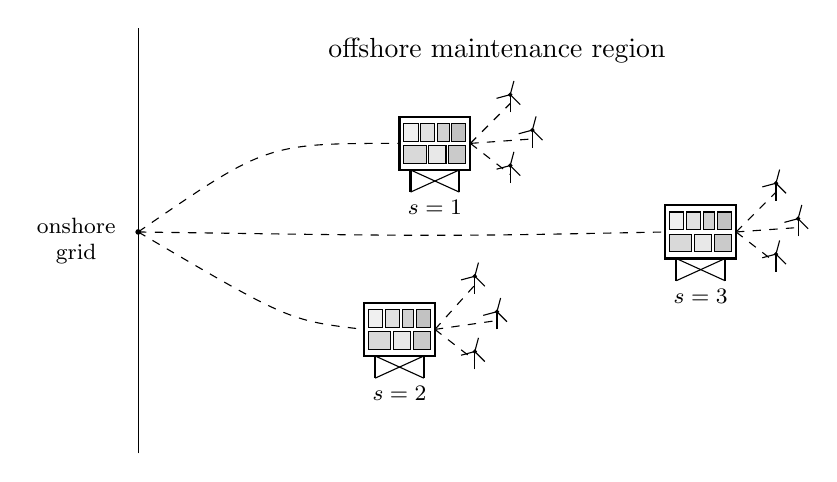
\begin{tikzpicture}[scale=0.5625, every node/.style={font=\footnotesize}]
  % Onshore grid, on the left, with a single shared connection point
  \draw (-1.9,-2) -- (-1.9,7.6);
  \node[align=center] at (-3.3,2.8) {onshore\\grid};
  \coordinate (shore) at (-1.9,3.0);
  \filldraw (shore) circle (0.05);

  % Seven components of a substation, as separate boxes inside the platform:
  % x0/y0/x1/y1/gray level/number, relative to the platform origin, platform 1.6 x 1.2.
  \def\complist{0.10/0.65/0.42/1.05/12/1, 0.48/0.65/0.80/1.05/24/2, 0.86/0.65/1.12/1.05/36/3, 1.18/0.65/1.50/1.05/48/4,
                0.10/0.15/0.60/0.55/30/5, 0.66/0.15/1.05/0.55/18/6, 1.11/0.15/1.50/0.55/42/7}
  % Small substation: platform with its seven components, on legs.
  \newcommand{\substation}[2]{%
    \begin{scope}[shift={(#1,#2)}]
      \draw[thick] (0.25,0) -- (0.25,-0.5); \draw[thick] (1.35,0) -- (1.35,-0.5);
      \draw (0.25,-0.5) -- (1.35,0); \draw (0.25,0) -- (1.35,-0.5);
      \draw[fill=white, thick] (0,0) rectangle (1.6,1.2);
      \foreach \a/\b/\c/\d/\g/\n in \complist { \draw[fill=figgray!\g] (\a,\b) rectangle (\c,\d); }
    \end{scope}}
  % Wind turbine at (x,y): mast and three blades.
  \newcommand{\turbine}[2]{%
    \draw (#1,#2-0.4) -- (#1,#2); \filldraw (#1,#2) circle (0.035);
    \foreach \ang in {75,195,315} { \draw (#1,#2) -- ++(\ang:0.32); }}

  % --- Substation s=1 (top), its turbines on the right ---
  \draw[dashed] (shore) .. controls (1.0,5.0) .. (4.0,5.0);
  \substation{4.0}{4.4}
  \node at (4.8,3.55) {$s=1$};
  \foreach \tx/\ty in {6.5/4.5, 7.0/5.3, 6.5/6.1} { \draw[dashed] (5.6,5.0) -- (\tx,\ty-0.2); \turbine{\tx}{\ty} }

  % --- Substation s=2 (bottom center), its turbines on the right ---
  \draw[dashed] (shore) .. controls (1.5,1.0) .. (3.2,0.8);
  \substation{3.2}{0.2}
  \node at (4.0,-0.65) {$s=2$};
  \foreach \tx/\ty in {5.7/0.3, 6.2/1.2, 5.7/2.0} { \draw[dashed] (4.8,0.8) -- (\tx,\ty-0.2); \turbine{\tx}{\ty} }

  % --- Substation s=3 (right), its turbines on the right ---
  \draw[dashed] (shore) .. controls (5.0,2.9) .. (10.0,3.0);
  \substation{10.0}{2.4}
  \node at (10.8,1.55) {$s=3$};
  \foreach \tx/\ty in {12.5/2.5, 13.0/3.3, 12.5/4.1} { \draw[dashed] (11.6,3.0) -- (\tx,\ty-0.2); \turbine{\tx}{\ty} }

  \node[font=\normalsize] at (6.2,7.1) {offshore maintenance region};
\end{tikzpicture}}
\caption{}
\label{fig:region-schematic}
\end{subfigure}
\hfill
\begin{subfigure}[b]{0.48\textwidth}
\centering
\resizebox{\linewidth}{!}{%
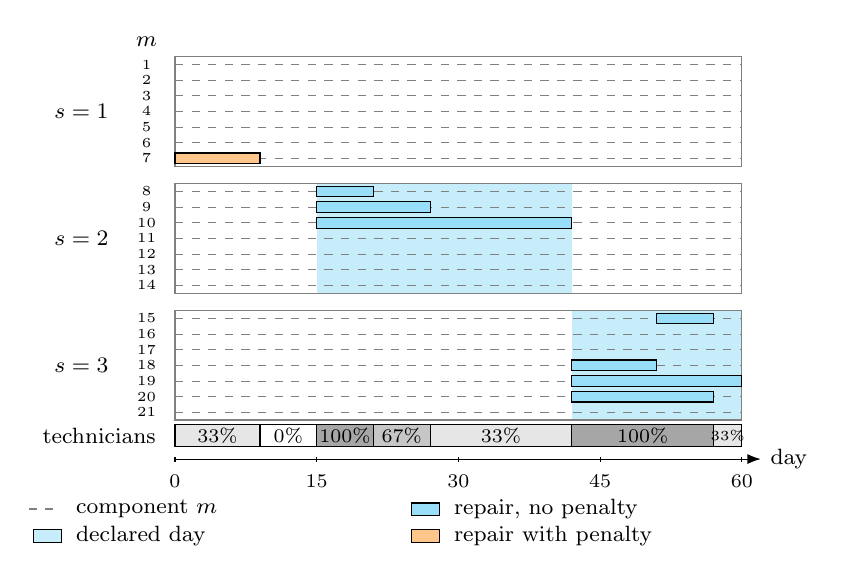
\begin{tikzpicture}[xscale=0.12, yscale=0.62, every node/.style={font=\footnotesize}]
  % Every repair requires a third of the technicians, so at most three repairs run
  % simultaneously.
  % --- Declared penalty-free days, per substation, only from day 16 (s=1: repair before day 16) ---
  \fill[cyan!22] (15,2.6) rectangle (42,4.84);
  \fill[cyan!22] (42,0) rectangle (60,2.24);

  % --- Band labels ---
  \node[anchor=east] at (-6,6.32) {$s=1$};
  \node[anchor=east] at (-6,3.72) {$s=2$};
  \node[anchor=east] at (-6,1.12) {$s=3$};
  \node at (-3,7.75) {$m$};

  % --- One dotted row per component (7 per substation), numbered globally ---
  \foreach \bandtop/\offset in {7.44/0,4.84/7,2.24/14} {
    \foreach \i in {1,...,7} {
      \pgfmathsetmacro\ry{\bandtop-(\i-0.5)*0.32}
      \pgfmathtruncatemacro\num{\offset+\i}
      \draw[dashed,figgray,line width=0.3pt] (0,\ry) -- (60,\ry);
      \node[font=\tiny] at (-3,\ry) {\num};
    }
    \draw[figgray] (0,\bandtop) rectangle (60,\bandtop-2.24);
  }

  % --- s=1: one repair, paid in full (before day 16, no penalty-free day can be declared) ---
  \pgfmathsetmacro\ry{7.44-(7-0.5)*0.32}
  \draw[fill=orange!45] (0,\ry-0.11) rectangle (9,\ry+0.11);
  % --- s=2: three repairs from day 16, within its penalty-free days ---
  \foreach \i/\e in {1/21,2/27,3/42} {
    \pgfmathsetmacro\ry{4.84-(\i-0.5)*0.32}
    \draw[fill=cyan!40] (15,\ry-0.11) rectangle (\e,\ry+0.11);
  }
  % --- s=3: four repairs, within its penalty-free days ---
  \foreach \i/\s/\e in {4/42/51,5/42/60,6/42/57,1/51/57} {
    \pgfmathsetmacro\ry{2.24-(\i-0.5)*0.32}
    \draw[fill=cyan!40] (\s,\ry-0.11) rectangle (\e,\ry+0.11);
  }

  % --- Region-wide technician occupancy ---
  \node[anchor=east] at (-1,-0.32) {technicians};
  \foreach \xa/\xb/\g in {0/9/20, 9/15/0, 15/21/70, 21/27/45, 27/42/20, 42/57/70, 57/60/20} {
    \draw[fill=figgray!\g] (\xa,-0.55) rectangle (\xb,-0.1);
  }
  \node[font=\scriptsize] at (4.5,-0.32) {33\%};
  \node[font=\scriptsize] at (12,-0.32) {0\%};
  \node[font=\scriptsize] at (18,-0.32) {100\%};
  \node[font=\scriptsize] at (24,-0.32) {67\%};
  \node[font=\scriptsize] at (34.5,-0.32) {33\%};
  \node[font=\scriptsize] at (49.5,-0.32) {100\%};
  \node[font=\fontsize{3.5}{4}\selectfont, inner sep=0pt] at (58.5,-0.32) {33\%};

  % --- Time axis ---
  \draw[-{Latex}] (0,-0.8) -- (62,-0.8) node[right] {day};
  \foreach \t in {0,15,30,45,60} {
    \draw (\t,-0.85) -- (\t,-0.75) node[below,yshift=-3pt]{\scriptsize \t};
  }

  % --- Legend ---
  \draw[dashed,figgray,line width=0.6pt] (-15.5,-1.82) -- (-12,-1.82);
  \node[anchor=west] at (-11.5,-1.82) {component $m$};
  \draw[fill=cyan!22] (-15,-2.5) rectangle (-12,-2.25);
  \node[anchor=west] at (-11.5,-2.37) {declared day};
  \draw[fill=cyan!40] (25,-1.95) rectangle (28,-1.7);
  \node[anchor=west] at (28.5,-1.82) {repair, no penalty};
  \draw[fill=orange!45] (25,-2.5) rectangle (28,-2.25);
  \node[anchor=west] at (28.5,-2.37) {repair with penalty};
\end{tikzpicture}}
\caption{}
\label{fig:schedule-schematic}
\end{subfigure}
\caption{The offshore substations maintenance problem. (a) A maintenance region: three substations, each with the
same seven components, each connecting its own cluster of wind turbines to the onshore grid. (b) A maintenance
schedule over a two-month period.}
\label{fig:problem}
\end{figure}

\paragraph{Literature gap.} Choosing the maintenance schedule that minimizes the cost of the current two-month period
can be written as a mixed-integer linear program (MILP). However, the TSO does not want to minimize the cost of the
current period, but the cost over the lifetime of the substations, since paying for maintenance now can prevent
failures later. The problem is therefore naturally a Markov Decision Process (MDP), whose state
contains the degradation state of every component and the remaining quota of every substation, and whose action is the
maintenance schedule of the region over the next two months. This MDP is hard to solve for three reasons.
\begin{itemize}
\item \emph{A factored state space.} The region is a multi-component system, in which every
component degrades according to its own dynamics, and the remaining quota of every substation evolves with its declared days. The joint state is the product of the states of these subsystems, so that the size of the state space
grows exponentially with their number, which is the curse of dimensionality of multi-component MDPs. With seven
components per substation, each with a few degradation levels, a single substation already has tens of thousands of
states, and a region of three substations more than $10^{14}$.
\item \emph{A non-separable cost.} The penalty that has to be paid for a substation is not the sum of penalties for its components. Its capacity
is limited by its most degraded component, and it is shut down on every day when one of its components is under
repair. The cost thus depends on the joint states of the components and on the days of their repairs, and not only on
the decisions taken for each component separately. The TSO therefore wants to group the repairs of the components of a
substation on the same days, and to cover them with penalty-free days, so as to minimize its downtime.
\item \emph{A combinatorial action space.} Since the cost depends on the days of the repairs, an action cannot only
state which components are repaired. It must represent the complete maintenance schedule of the region, that is, for
every component, whether it is repaired and on which day the repair starts, and, for every substation, which days are
declared penalty-free, so that the number of actions grows exponentially with the number of components. The schedule
must moreover satisfy operational constraints, such as the number of technicians shared by the region and the quota of
penalty-free days of each substation, which link the decisions of all the components.
\end{itemize}

Two classes of structured MDPs of the literature are close to our problem and are known to admit tractable LP
approximations. Both consider $M$ subsystems, indexed by $m \in [M] := \{1,\ldots,M\}$, evolving over $T$ time steps.
Subsystem $m$ has a state $x_m$ in a finite set $\mathcal{X}_m$, and the joint state is $x_\otimes = (x_1,\ldots,x_M)
\in \mathcal{X}_\otimes := \mathcal{X}_1 \times \cdots \times \mathcal{X}_M$.

\begin{definition}[Decomposable MDP (D-MDP)~\cite{bertsimas2016}]
\label{def:dmdp}
A single joint action $a$, common to every subsystem, is chosen at each time step from a finite action space $\mathcal{A}$.
Conditionally on $a$, subsystem $m$ transitions from $x_m$ to $x_m'$ with probability $p_m(x_m' \mid x_m, a)$,
independently of the other subsystems, and incurs a cost $c_m(x_m,a)$. The joint cost is
$c_\otimes(x_\otimes, a) = \sum_{m \in [M]} c_m(x_m, a)$.
\end{definition}

\begin{definition}[Weakly coupled MDP (W-MDP)~\cite{hawkins2003}]
\label{def:wmdp}
Each subsystem has its own local action $a_m$ in a finite set $\mathcal{A}_m$. Conditionally on $a_m$, subsystem $m$
transitions from $x_m$ to $x_m'$ with probability $p_m(x_m' \mid x_m, a_m)$, independently of the other subsystems,
and incurs a cost $c_m(x_m,a_m)$. The joint cost is $c_\otimes(x_\otimes,(a_m)_{m}) = \sum_{m \in [M]} c_m(x_m,a_m)$.
The local actions are coupled by $K$ additive linking constraints $\sum_{m \in [M]} D_m(a_m) \le d$, for a budget
$d \in \mathbb{R}^K$ and resource consumption functions $D_m$.
\end{definition}

Our problem shares the structure common to these two classes, since, given the maintenance decisions, components
degrade independently of one another. The methods developed for them can however not be applied directly, and must be
adapted, for the following reasons: the cost is not separable, the joint action cannot be enumerated (which makes the standard 
methods for decomposable intractable MDPs), and the coupling is not only through additive constraints (which prevents applying
the standard methods for weakly coupled MDPs).

\subsection{Literature review}
\label{sec:literature-review}

\paragraph{Methodologies for MDPs with combinatorial actions.}
\begin{comment}
Commentaire cyrille: présenter mathématiquement ce que sont les D-MDPs et W-MDPs. Expliquer le LP pour les MDPs généraux, on ne peut pas résoudre direcetement quand il est gros, quand il y a une structre comme dans le cas des W-MDPs ou D-MDPs on approxime. Attention la fonction valeur prend en entrée l'état seulement, pas le couple état action. On ne comprends pas ce que sont les variables du primal. Il n'est pas focement nécessaire de définir le primal si on n'en parle pas ensuite. Faire un tableau pour préciser les différences entre weakly coupled mdps, decomposable MDPs... (formalism, LP)
\end{comment}
We review the methods used in the literature for problems with a similar structure, in which several subsystems
evolve over time and are coupled at each time step by a combinatorial decision. A common approach is to decouple the
subsystem-level optimization from the joint optimization. The decisions of each subsystem are first optimized in
isolation, and then enforced as constraints in the joint problem, as in~\cite{Kingsman2020} or~\cite{Mankowska2014}. 
Alternatively, the joint optimization penalizes deviations from the subsystem-level solution, as in~\cite{Irawan2017, lopezsantana2023}, or the two levels are solved
alternately until convergence~\cite{LopezSantana2016}. Another approach is
to solve both levels jointly, with tailored metaheuristics such as ant colony optimization~\cite{allal2021} or genetic
algorithms~\cite{Camci2015}. Finally, reinforcement learning methods have recently been adapted to combinatorial action
spaces, by combining learning with combinatorial optimization~\cite{Hoppe2025SRL} or by embedding a learned value
function into a mixed-integer program that selects the action~\cite{xu2025combinatorial, delarue2020reinforcement}.
These methods are generic, but they can suffer from instability, and training the policy can be a heavy process.

\paragraph{Linear programming for MDPs.}
\label{sec:lp-review}
In this paper, we propose a linear programming approach. It is well known~\cite{manne_linear_1960} that any MDP can be reformulated exactly as a
linear program: the primal LP has one variable per state, representing its value, while its dual has one
variable per state-action pair, representing the probability of visiting that pair. This LP does not scale: it
becomes intractable as soon as the state space or the action space is too large. Linear programming is nonetheless
a well established tool for W-MDPs and D-MDPs, for which a good, tractable approximation of the LP (primal or dual)
can be obtained by exploiting the structure of the MDP. W-MDPs generalize the \emph{restless multi-armed bandit} (RMAB) framework. In RMABs, each subsystem action is binary, either active or passive, and there is a single constraint: at most $K$ subsystems, or arms, can be activated out of $M$.
For RMABs, Whittle~\cite{whittle1988} proposed relaxing the coupling constraint to hold only in expectation
and dualizing it with a state-independent multiplier. This decouples the problem into independent one-armed
MDPs and yields the Whittle index policy, later shown to be asymptotically optimal as the number of arms
grows, under some conditions. Building on this idea, Hawkins~\cite{hawkins2003} applies Lagrangian
relaxation to more general W-MDPs, showing that the resulting bound can be computed exactly
via a primal LP whose size grows only linearly with the number of subproblems, with
variables that can be interpreted as subsystem values whose sum approximates the value
function. Adelman and Mersereau~\cite{AdelmanMersereau2008} show that the dual of this LP has variables that can instead be interpreted as
the discounted expected fraction of time that each subsystem spends in each state-action pair, subject to
flow constraints at subsystem level and an expected resource constraint. In this paper, we choose to work with the dual: we call \emph{fluid LP} any such
dual LP approximation of an MDP whose variables include the probabilities of subsystem state/action pairs. Bertsimas and
Niño-Mora~\cite{bertsimasninomora2000} introduce a hierarchy of fluid LPs for RMABs,
where each successive level incorporates higher-order moments of the distribution of the states and actions,
yielding increasingly tight bounds on the optimal value at the cost of larger and more complex LP
formulations. In addition to providing a bound on the value of the MDP, fluid LPs can be used to construct policies. One possibility is to solve a single MDP and derive a policy from it for all time steps. However, the resulting probabilities do not always correspond to a feasible policy, in which case a repair heuristic \cite{DAeth2023HospitalScheduling} can be introduced. Another possibility is to solve the LP at each time step and apply a greedy policy with respect to the value function estimate provided by the LP, which often results in better performance \cite{gast2022lpupdate}. The authors in~\cite{brownzhang2022, DAeth2023HospitalScheduling} prove asymptotic optimality
guarantees when the number of subsystems tends to infinity for a fluid policy for a finite-horizon W-MDP or group W-MDP (where subsystems are partitioned into a small number of groups sharing identical dynamics and rewards). Bertsimas and Mišić~\cite{bertsimas2016}
propose a fluid LP for D-MDPs in an infinite-horizon setting. The D-MDP setting seems to have received
less attention in the literature than W-MDPs, and to the best of our knowledge, no
performance guarantee is available for the resulting fluid policy as the number of subsystems grows. Another difficulty regarding D-MDPs is to build tractable approximations when the joint action space is large: in the LP formulations proposed in~\cite{bertsimas2016}, the number of variables is proportional to the size of the action space. Liu,
Wiesemann, and Yue~\cite{liuwiesemannyue2024} study factored MDPs with low-scope transition
probabilities and reward, in which the system decomposes into subsystems whose transition probabilities
depend only on a small subset of other subsystems, and whose reward decomposes into a sum of terms
depending on the joint action and the state of a small set of subsystems. They solve an approximation of the primal LP via a cutting-plane scheme for infinite-horizon
discounted factored MDPs, exploiting the
sparse dependence on a MILP representable feature vector to keep the
LP tractable. They study subsystem decomposable actions subject to a resource constraint, but do not
consider more structured joint actions, which we propose to study in this paper. To the best of our
knowledge, tractable LP formulations for decomposable MDPs with general combinatorial action spaces have
not yet been established.

\subsection{Contributions and outline}

Our contribution is twofold. First, we propose a modelisation for the offshore substations maintenance
problem and a method to solve it quickly. Second, we generalize the
fluid approximations of D-MDPs and W-MDPs toMDPs made of subsystems coupled by a combinatorial joint
action. The rest of the paper is organized as follows. Section~\ref{sec:problem-statement} models the offshore substations maintenance problem as an MDP.
Section~\ref{sec:combinatorial} presents a general method to build LP approximations of MDPs, in connection with the
theory of probabilistic graphical models. Section~\ref{sec:hierarchy} discusses the quality of these
approximations, and then presents two methods to improve the approximation, both drawn from the
probabilistic graphical models literature.
Section~\ref{sec:numerics} provides a numerical evaluation of these methods on the offshore substations maintenance problem.

\section{MDP model}
\label{sec:problem-statement}


\subsection{Problem statement}

We now formalize the problem described in Section~\ref{sec:intro-application}. A region groups $S$ substations, indexed by $s \in [S]$. Every two months, the TSO must declare to the
producer which days of the following two-month period it wants to declare penalty-free. Maintenance for the whole
two-month period is therefore planned entirely at its start. For simplicity, we assume that the degradation
probabilities and the costs are stationary, although in practice they vary with the seasons. Likewise, the only
operational constraint we consider is the capacity of the team of technicians shared by the region, although other
constraints, such as labor regulations or safety rules, would have to be imposed in practice. We model the maintenance of offshore electrical substations as an MDP with a
time step of two months, and the components listed in Table~\ref{tab:mdp-components} and detailed in
Section~\ref{sec:model-details}.

\begin{table}[h]
\centering
\begin{tabular}{lp{6.2cm}p{2.8cm}}
\toprule
MDP component & Description & Notation \\
\midrule
Time step & Two months (60 days) & $t$ \\
\midrule
Horizon & 20 years (120 time steps) & $T$ \\
\midrule
\multirow{2}{*}{State}
 & $\bullet$ Degradation states of every key component within every substation of the region & $(n_m)_{m \in [M]}$ \\
 & $\bullet$ Remaining quota per substation & $(k^s)_{s \in [S]}$ \\
\midrule
\multirow{2}{*}{Action}
 & $\bullet$ Maintenance schedule for every substation & $(\tau^{\text{start}}_m)_{m \in [M]}$ \\
 & $\bullet$ Declared days for every substation & $(\text{Free}^s)_{s \in [S]}$ \\
\midrule
\multirow{2}{*}{Cost}
 & $\bullet$ Penalties for every substation & $(c^{\mathrm{pen},s})_{s \in [S]}$ \\
 & $\bullet$ Replacement costs of the components maintained & $(c^{\mathrm{rep}}_m)_{m \in [M]}$ \\
\bottomrule
\end{tabular}
\caption{Components of the offshore substations maintenance MDP.}
\label{tab:mdp-components}
\end{table}

\label{sec:model-details}
\label{sec:decomposable-MDPs}

\paragraph{State.} We include in the state the information necessary to make the maintenance decision: the degradation state of every component, and the remaining quota of every substation.
We assume that every substation has the same design. We represent only each substation's key
components in the MDP, meaning those whose failure can affect its evacuation capacity. Every substation has the same
$M_0$ key components, for example a converter, a transformer, or a cooling system, for a total of $M = S \cdot M_0$
components region-wide, indexed globally by $m \in [M]$. We write $\mathcal{M}^s \subseteq [M]$ for the components
of substation $s$, and $s(m)$ for the substation of component $m$.
Each component $m$ degrades on its own discrete degradation scale: we write $n_m \in [N_m]$ its \emph{degradation
state}, from new ($n_m=1$) to failed ($n_m=N_m$). We write $K_0$ the annual quota of penalty-free days of a substation, assumed to be the same
for every substation, and $k^s \in [0:K_0]$ the \emph{remaining quota} of substation $s$, that is, the number of penalty-free days it can still declare in the current year. The state of the MDP at the start of a period is then
\[
x_\otimes \ =\ \big( (n_m)_{m \in [M]},\ (k^s)_{s \in [S]} \big) \ \in\ \mathcal{X}_\otimes := [N_1] \times \cdots \times [N_M] \times [0:K_0]^S.
\]
The system starts in a fixed initial state $\mathbf{x}_\otimes = \big( (\mathbf{n}_m)_{m \in [M]}, (\mathbf{k}^s)_{s \in
[S]} \big) \in \mathcal{X}_\otimes$, which is the current state of the region when a decision has to be made.


\paragraph{Joint action.} The joint action is the global maintenance schedule for the two months period. The technician capacity constraint and the penalty-free quota are enforced day by day. We
thus represent the maintenance schedule at a daily granularity, and assume that each two-month period has 60 days for
simplicity. Repairing component $m$ takes $d_m \ge 1$ workdays, and requires a fraction $\rho_m$ of the available technician workforce on
each of those days. A repair can start on any day of the period. We write $\delta_m \in \{0,1\}$ the \emph{maintenance decision} of component $m$, $\delta_m = 1$ meaning that
component $m$ is repaired during the period, and $\tau^{\text{start}}_m \in \{0\} \cup [60]$ the
\emph{start day} of its repair, $\tau^{\text{start}}_m = 0$ meaning that component $m$ is not repaired. The start day
must leave enough time for the repair to complete within the period, and is consistent with the maintenance decision:
\begin{equation}
\label{eq:intro-start-feasible}
\tau^{\text{start}}_m \neq 0 \ \implies\ \tau^{\text{start}}_m + d_m - 1 \ \le\ 60,
\end{equation}
\begin{equation}
\label{eq:intro-am-link}
\delta_m \ =\ \mathds{1}_{\{\tau^{\text{start}}_m \neq 0\} }.
\end{equation}
The producers must be notified of the penalty-free days in advance, so that the first $L$ days of the period cannot
be declared penalty-free ($L = 15$). We write $\text{Free}^s \subseteq \{L+1, \ldots, 60\}$ the \emph{declared days} of substation $s$, that is, the set of days declared penalty-free for it, and $\kappa^s := |\text{Free}^s|$ their number. The declaration is
subject to the \emph{quota constraint}
\begin{equation}
\label{eq:intro-quota-constraint}
\kappa^s \ \le\ k^s \qquad \forall s \in [S].
\end{equation}
The \emph{repair set} $\text{Repair}_\tau \subseteq [M]$ is the set of
components under repair on day $\tau$,
\begin{equation}
\label{eq:intro-repair}
\text{Repair}_\tau \ =\ \big\{ m \in [M] : \tau^{\text{start}}_m \neq 0,\ \tau^{\text{start}}_m \le \tau
\le \tau^{\text{start}}_m + d_m - 1 \big\}.
\end{equation}
The technician shares of the components under repair on a
given day cannot exceed the available workforce, which gives the \emph{technician capacity constraint}
\begin{equation}
\label{eq:intro-technicians}
\sum_{m \in \text{Repair}_\tau} \rho_m \ \le\ 1 \qquad \forall \tau \in [60].
\end{equation}
Finally, the \emph{maintenance indicator} $m^s_\tau \in \{0,1\}$ is equal to $1$ if at least one component of
substation $s$ is under repair on day $\tau$,
\begin{equation}
\label{eq:intro-maintenance-indicator}
m^s_\tau \ =\ \mathds{1}_{\{\mathcal{M}^s \cap \text{Repair}_\tau\neq
\emptyset\}}.
\end{equation}
The action variables for the period are the start days $\tau^{\text{start}}_m$ and the sets $\text{Free}^s$ of declared days. The maintenance decisions $\delta_m$, the repair sets $\text{Repair}_\tau$ and the maintenance
indicators $m^s_\tau$ are uniquely determined by them, but are useful to write the cost. 

\paragraph{Transitions.} We need to define the transition for the two elements of the state, the degradation states and the remaining quotas. 
We write $p_m(n'_m \mid n_m, \delta_m)$ the probability that component $m$ is in state
$n'_m$ at the start of the next period, given that it enters the current period in state $n_m$ and that its
maintenance decision is $\delta_m$. If $\delta_m=0$, the component degrades
stochastically over the period according to this transition kernel. If $\delta_m=1$, it is repaired and
deterministically returns to the new state, so $p_m(1 \mid n_m, 1) = 1$ for every $n_m$. The components degrade
 independently of one another. The remaining quota of
substation $s$ evolves deterministically as $k'^s = \phi_t\big(k^s, \kappa^s\big)$,
where the \emph{quota dynamics} $\phi_t$ is
\begin{equation}
\label{eq:intro-quota-dynamics}
\phi_t(k, \kappa) \ =\
\begin{cases}
K_0 & \text{if period } t+1 \text{ is the first period of a new year,} \\
k - \kappa & \text{otherwise.}
\end{cases}
\end{equation}
The quota thus resets to $K_0$ at the start of every year. By the independence of the components
and~\eqref{eq:intro-quota-dynamics}, the transition probabilities of the MDP are
\begin{equation}
\label{eq:joint-transition}
p_\otimes(x'_\otimes \mid x_\otimes, b) \ =\ \prod_{m \in [M]} p_m\big(n'_m \mid n_m, \delta_m\big)
\ \prod_{s \in [S]} \mathds{1}_{\{k'^s = \phi_t(k^s, \kappa^s)\}},
\end{equation}
where $\delta_m$ and $\kappa^s$ are those of the joint action $b$.
Given the joint action, the components and the quotas thus evolve independently of one another. The dependence of
$\phi_t$ on $t$ makes the MDP non-stationary. To keep notations light we omit the index $t$ of the transition
probabilities, and all the methods presented in this paper extend directly to the non-stationary case.

\paragraph{Cost.} The cost over a time step is the sum of penalties and replacement costs paid for each component that
has to be changed. To express the penalties for every day within the period, we need to represent the state of every component 
on every day of the period. From the state $n_m$ of component $m$ at the beginning of the period and its start day
$\tau^{\text{start}}_m$, we deduce its state $\tilde{n}_{m,\tau}$ on any day $\tau$ of the period,
\[
\tilde{n}_{m,\tau} \ =\
\begin{cases}
1 & \text{if } \tau^{\text{start}}_m \neq 0 \text{ and } \tau \ge \tau^{\text{start}}_m + d_m, \\
n_m & \text{otherwise},
\end{cases}
\]
equal to $n_m$ until the repair, if any, is complete, and to the new state $1$ from then on. We associate to each
component $m$ and degradation state $n_m$ a \emph{capacity loss} $\ell_m(n_m) \in [0,1]$, non-decreasing in $n_m$.
We assume that the components of a substation are connected in series: the power exported by the substation flows
successively through every one of them (converter, transformer, cooling system, etc.), so that each component limits
the power that can go through the whole chain. The capacity of the substation is bottlenecked by its most degraded
component, and its capacity loss is the largest of the capacity losses of its components, as illustrated in
Figure~\ref{fig:series}. This holds except on
maintenance days, when the substation is shut down entirely for safety regardless of which components are being
repaired.

\begin{figure}[h]
\centering
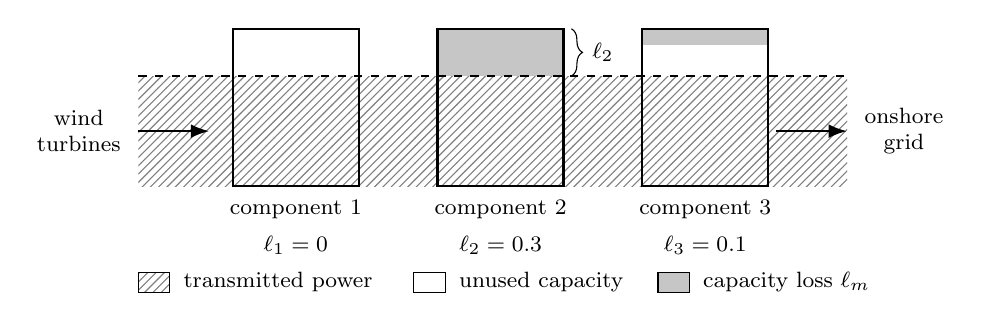
\begin{tikzpicture}[x=1cm, y=1cm, every node/.style={font=\footnotesize}]
  % Three components in series, of height 2 (full capacity). The gray part of a component is its capacity loss
  % ell_m, the white part the power it can carry. The power flow (hatched) is limited by the narrowest component.
  \def\H{2}
  % power flow, of height 2 (1 - max ell) = 1.4, through the whole chain
  \fill[pattern=north east lines, pattern color=gray] (-0.6,0) rectangle (8.4,1.4);
  \draw[-{Latex}, thick] (-0.6,0.7) -- (0.3,0.7);
  \draw[-{Latex}, thick] (7.5,0.7) -- (8.4,0.7);
  \node[anchor=east, align=center] at (-0.7,0.7) {wind\\turbines};
  \node[anchor=west, align=center] at (8.5,0.7) {onshore\\grid};
  \foreach \x/\l/\lab/\n in {0.6/0/0/1, 3.2/0.3/0.3/2, 5.8/0.1/0.1/3} {
    \pgfmathsetmacro\top{\H*(1-\l)}
    \fill[white] (\x,1.4) rectangle (\x+1.6,\H);
    \fill[figgray!45] (\x,\top) rectangle (\x+1.6,\H);
    \draw[thick] (\x,0) rectangle (\x+1.6,\H);
    \node at (\x+0.8,-0.3) {component $\n$};
    \node at (\x+0.8,-0.75) {$\ell_\n = \lab$};
  }
  \draw[dashed] (-0.6,1.4) -- (8.4,1.4);
  \draw[decorate, decoration={brace, amplitude=4pt}] (4.9,2) -- (4.9,1.4) node[midway, right=4pt] {$\ell_2$};
  % legend
  \fill[pattern=north east lines, pattern color=gray] (-0.6,-1.35) rectangle (-0.2,-1.1); \draw (-0.6,-1.35) rectangle (-0.2,-1.1);
  \node[anchor=west] at (-0.15,-1.22) {transmitted power};
  \fill[white] (2.9,-1.35) rectangle (3.3,-1.1); \draw (2.9,-1.35) rectangle (3.3,-1.1);
  \node[anchor=west] at (3.35,-1.22) {unused capacity};
  \fill[figgray!45] (6.0,-1.35) rectangle (6.4,-1.1); \draw (6.0,-1.35) rectangle (6.4,-1.1);
  \node[anchor=west] at (6.45,-1.22) {capacity loss $\ell_m$};
\end{tikzpicture}
\caption{Components of a substation connected in series. The power produced by the wind turbines flows through every
component before reaching the onshore grid, and each component can only carry the fraction $1 - \ell_m$ of the full
power. The power transmitted to the grid (hatched) is thus limited by the most degraded component, here component
$2$, and is $\min_m (1 - \ell_m) = 1 - \max_m \ell_m = 0.7$. The capacity loss of the substation is
$\max_m \ell_m = 0.3$, and not the sum $0.4$ of the capacity losses.}
\label{fig:series}
\end{figure}

\emph{Substation $s$'s joint capacity loss} on day $\tau$, $\ell^s_\tau \in [0,1]$, is then
\begin{equation}
\label{eq:intro-capacity-loss}
\ell^s_\tau \ =\ m^s_\tau \ +\ \big(1 - m^s_\tau\big)
\max_{m \in \mathcal{M}^s} \ell_m\big(\tilde{n}_{m,\tau}\big).
\end{equation}
The penalty that has to be paid for a substation is
proportional to the capacity loss outside of the declared days. We assume that the \emph{penalty per unit
of capacity lost} is equal to $1$, which fixes the unit of cost. Substation $s$'s \emph{penalty} over the period,
$c^{\mathrm{pen},s}$, is
\begin{equation}
\label{eq:intro-penalty}
c^{\mathrm{pen},s} \ :=\ \sum_{\tau \notin \text{Free}^s} \ell^s_\tau.
\end{equation}
We write $c^{\mathrm{rep}}_m$ the \emph{replacement cost} of component $m$. The \emph{total cost} over a period,
$c^{\mathrm{tot}}$, is the sum of the replacement costs of the components repaired and of the penalties of the substations,
\begin{equation}
\label{eq:intro-cost}
c^{\mathrm{tot}} \ =\ \sum_{m \in [M]\,:\, \delta_m = 1} c^{\mathrm{rep}}_m
\ +\ \sum_{s \in [S]} c^{\mathrm{pen},s}.
\end{equation}


\paragraph{Joint actions and joint cost.} We write $b$ the \emph{joint action}, i.e., the start days
$\tau^{\text{start}}_m$ and the sets $\text{Free}^s$. The joint action is thus the \emph{maintenance schedule} of the
region over the period, which states which components are repaired, on which days, and the declared days of every substation. We write $\mathcal{B}(x_\otimes)$ the set of the joint actions that
satisfy the constraints above in state $x_\otimes$, and $\mathcal{B}$ the set of the joint actions that satisfy them
without the quota constraint~\eqref{eq:intro-quota-constraint}. The \emph{joint cost} $c_\otimes(x_\otimes, b)$ is the
total cost~\eqref{eq:intro-cost} of the joint action $b$ in state $x_\otimes$.

\paragraph{Policies and objective.}
Markov policies attain the optimal value of a finite-horizon MDP with finite state and action spaces
\cite[Theorem 4.4.2]{puterman1994}. We thus seek a time-dependent Markov policy $\pi = (\pi_t)_{t \in [T]}$, where $\pi_t$
maps each state $x_\otimes$ to a distribution over $\mathcal{B}(x_\otimes)$. Together with the initial state
$\mathbf{x}_\otimes$ defined above and the transition probabilities $p_\otimes$, a policy induces a stochastic process
$(X_{\otimes,t}, B_t)_{t \in [T]}$ over state-action pairs. Throughout the paper, we denote random variables by
uppercase letters and the values they take by lowercase letters, with the index $t$ of the time step. The policy is chosen so as to minimize the expected total cost
\[
\min_\pi J(\pi) = \mathbb{E}_\pi \Bigg[ \sum_{t \in [T]} c_\otimes(X_{\otimes,t}, B_t) \ \Big| \ X_{{\otimes},1} = \mathbf{x}_{\otimes} \Bigg].
\]
We denote by $J^\star = \min_\pi J(\pi)$ its optimal value. Although an optimal deterministic policy always exists,
we allow for stochastic policies. 


\subsection{Relation to decomposable and weakly coupled MDPs}
\label{sec:decomposable-weakly-coupled}
\label{sec:local-variables}

The MDP described above has three levels: a global level, a substation level and a component level, as represented on figure~\ref{fig:mdp-structure}. 
The maintenance schedule is represented at the global level. The cost, the remaining quota and the declared days are represented at the substation level. 
The degradation state and the maintenance decisions are represented at the component level (or local level).

\begin{figure}[!htb]
\centering
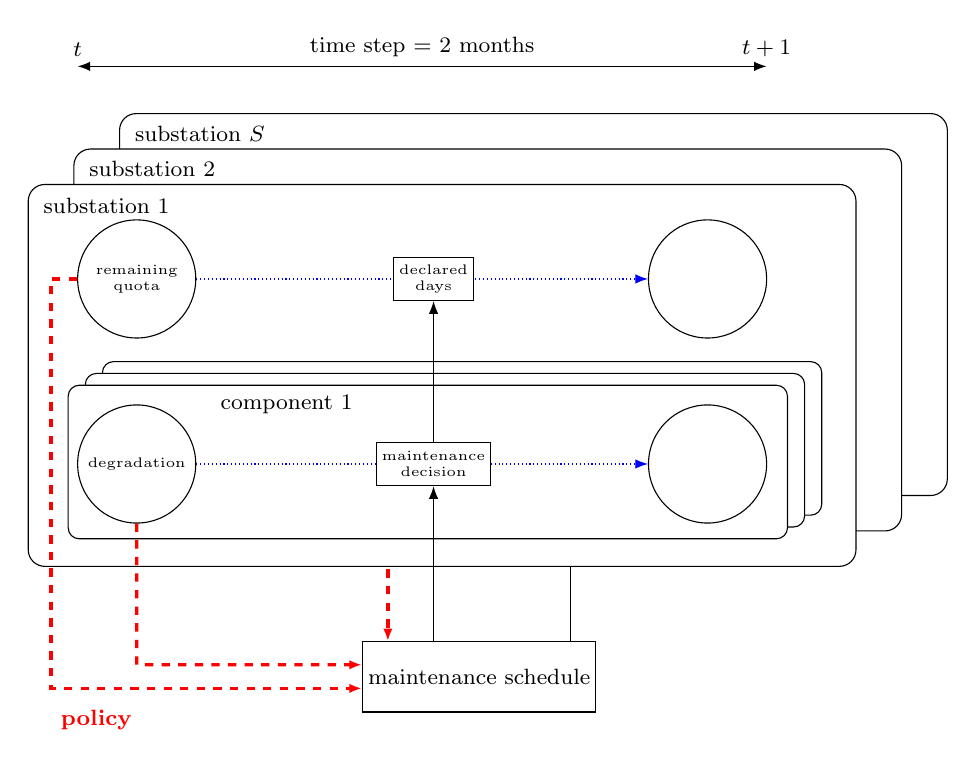
\begin{tikzpicture}[x=1.45cm, >={Latex[length=1.6mm]},
    st/.style={draw, circle, minimum size=1.5cm, inner sep=0pt, font=\tiny, align=center},
    ac/.style={draw, fill=white, rectangle, minimum width=0.7cm, minimum height=0.55cm, inner sep=2pt, font=\tiny,
               align=center},
    plate/.style={draw, fill=white, rounded corners=6pt},
    comp/.style={draw, fill=white, rounded corners=4pt},
    lab/.style={font=\footnotesize},
    dyn/.style={->, densely dotted, blue},
    pol/.style={->, dashed, red, very thick},
    det/.style={->}]
  % --- time step ---
  % from the outer edge of the state circles to the outer edge of the next state circles (radius 0.75cm)
  \draw[<->] ([xshift=-0.75cm]0,2.75) node[above, lab] {$t$} -- ([xshift=0.75cm]5.0,2.75) node[above, lab] {$t+1$}
    node[midway, above, lab] {time step $=$ 2 months};

  % --- one plate per substation, stacked as in plate notation: substation 1 in front, substations 2 to S behind it.
  % In the plate of substation 1, the quota of the substation, and one frame per component, the frames of the
  % components being stacked in the same way (component 1 in front). The action variables are drawn on the dynamics
  % arrows between the states, which are drawn first and hidden by them, so that the arrow from the action to the next
  % state is the end of the arrow between the states.
  \draw[plate] (-0.15,-2.7) rectangle (7.1,2.15);
  \node[lab, anchor=north west] at (-0.1,2.12) {substation $S$};
  \draw[plate] (-0.55,-3.15) rectangle (6.7,1.7);
  \node[lab, anchor=north west] at (-0.5,1.67) {substation $2$};
  % links of substation S with B_t, drawn before the plate of substation 1, which hides them
  \draw[pol] (2.2,1.0) -- (2.2,-4.55);
  \draw[det] (3.8,-4.55) -- (3.8,1.0);
  \draw[plate] (-0.95,-3.6) rectangle (6.3,1.25);
  \node[lab, anchor=north west] at (-0.9,1.2) {substation $1$};
  \node[st] (k)  at (0,0.05)    {remaining\\quota};
  \node[st] (kk) at (5.0,0.05)  {};
  \draw[dyn] (k) -- (kk);
  \node[ac] (ka) at (2.6,0.05)  {declared\\days};
  \draw[comp] (-0.3,-2.95) rectangle (6.0,-1.0);
  \draw[comp] (-0.45,-3.1) rectangle (5.85,-1.15);
  \draw[comp] (-0.6,-3.25) rectangle (5.7,-1.3);
  \node[lab, anchor=west] at (0.65,-1.55) {component $1$};
  \node[st] (n)  at (0,-2.3)     {degradation};
  \node[st] (nn) at (5.0,-2.3)   {};
  \draw[dyn] (n) -- (nn);
  \node[ac] (d)  at (2.6,-2.3)   {maintenance\\decision};

  % --- joint action, below the plates. The links of substation 1 go to its variables: the policy reads its states
  % (left), and B_t sets its actions (from below, through Delta up to |FREE|).
  \node[ac, minimum width=2.4cm, minimum height=0.9cm, font=\footnotesize] (b) at (3.0,-5.0) {maintenance schedule};
  \draw[pol] (n.south) -- (0,-4.85) -- ([yshift=0.15cm]b.west);
  \draw[pol] (k.west) -- (-0.75,0.05) -- (-0.75,-5.15) -- ([yshift=-0.15cm]b.west);
  \draw[det] (2.6,-4.55) -- (d.south);
  \draw[det] (d.north) -- (ka.south);

  \node[anchor=north west, font=\footnotesize\bfseries, text=red] at (-0.75,-5.3) {policy};
\end{tikzpicture}
\caption{One time step of the offshore substations maintenance MDP.}
\label{fig:bayesian-network}
\label{fig:mdp-structure}
\end{figure}
The tractability of numerical methods for D-MDPs and W-MDPs relies on the decomposition of the MDP into subsystems. We show that we can recover
a similar structure for the MDP of Section~\ref{sec:problem-statement}, despite the 3 level structure presented above. We chose to decompose the system
at the component level, defining one subsystem per 
component. The maintenance decision for a component might not depend only on its degradation state, we also have to 
consider the remaining quota of the substation. We therefore define the \emph{local state} of a component $m$ at $t$ as the pair
made of its degradation state and of the remaining quota of its substation, it is written $X_{m,t}$ . 
We also define its \emph{local action} as the pair
made of its maintenance decision and of the number of declared days of its substation it is written $A_{m,t}$:
\begin{align*}
X_{m,t} &:= \big(N_{m,t}, K^{s(m)}_t\big) \in \mathcal{X}_m := [N_m] \times [0:K_0], \\
A_{m,t} &:= \big(\Delta_{m,t}, |\text{FREE}^{s(m)}_t|\big) \in \mathcal{A}_m := \{0,1\} \times [0:K_0].
\end{align*}
We write $x = (n, k)$ and $a = (\delta, \kappa)$ their values, and $\mathbf{x}_m := (\mathbf{n}_m,
\mathbf{k}^{s(m)})$ the initial local state of component $m$. The quota constraint~\eqref{eq:intro-quota-constraint}
restricts the local actions in the local state $x$ to the set
\[
\mathcal{A}_m(x) := \big\{ (\delta, \kappa) \in \mathcal{A}_m \mid \kappa \le k \big\},
\]
and, by~\eqref{eq:joint-transition}, the local state evolves according to
\[
p_m(x' \mid x, a) := p_m(n' \mid n, \delta)\, \mathds{1}_{\{k' = \phi_t(k, \kappa)\}},
\]
which only depends on the local state and on the local action of component $m$. The local actions can be deduced from the
joint action. For a joint action $b$, the local action of component $m$ is
\[
A_m(b) := \big(\delta_m(b), \kappa^{s(m)}(b)\big),
\]
where $\delta_m(b) \in \{0,1\}$ is the maintenance decision of component $m$, equal to $1$ if $m$ is maintained in the
maintenance schedule $b$, and
$\kappa^s(b) = |\text{Free}^s|$ is the number of declared days of substation $s$ in $b$. Unlike in
weakly coupled and decomposable MDPs, however, the cost is not a sum of local costs that each depend only on the local
state and the local action of one component, since the penalty of a substation depends jointly on the degradation
states of all its components within a substation. Section~\ref{sec:intro-approx} explains how we handle this difficulty.


\section{Fluid approximations}
\label{sec:combinatorial}
Linear programming is the standard tool to build tractable approximations of W-MDPs and
D-MDPs~\cite{AdelmanMersereau2008, bertsimas2016}. We follow the same approach for the
MDP of Section~\ref{sec:problem-statement}. Section~\ref{sec:fluid-lp} presents an exact LP, whose optimal value is
the optimal value of the MDP but which is not tractable. Section~\ref{sec:marginal-polytopes} presents a general method
to build LP approximations of the MDP. We build our approximations by making two independent choices, summarized in Table~\ref{tab:approximations}.
The first choice is the representation of the joint action. The Joint fluid LP (JFLP), inspired by the fluid formulation of D-MDPs, represents its complete distribution, which requires column generation (Section~\ref{sec:full-fluid}). The
Compact fluid LP (CFLP), inspired by the fluid formulation of W-MDPs, only represents its mean values, and imposes the
constraints on the joint action in expectation (Section~\ref{sec:compact}). The second choice is the decomposition of
the MDP into subsystems. In the decomposition of Section~\ref{sec:local-variables}, the remaining quota of a 
substation is included in the local state of each of its components. In a lighter decomposition, it forms its 
own subsystem (Section~\ref{sec:quota-subsystem}). Both representations of the joint action apply to both decompositions,
which gives four approximations in total.

\begin{table}[h]
\centering
\small
\renewcommand{\arraystretch}{1.2}
\begin{tabular}{|l|c|c|}
\hline
 & \multicolumn{2}{c|}{\textbf{Representation of the joint action}} \\
\cline{2-3}
\textbf{Decomposition} & Complete distribution of $B_t$ & Marginals of $B_t$ \\
\hline
Remaining quota in every subsystem & Joint fluid LP (JFLP) & Compact fluid LP (CFLP) \\
 & Section~\ref{sec:full-fluid} & Section~\ref{sec:compact} \\
\hline
Remaining quota as own subsystem & JFLP-Q & CFLP-Q \\
 & Section~\ref{sec:quota-subsystem} & Section~\ref{sec:quota-subsystem} \\
\hline
\end{tabular}
\caption{The four approximations, according to the decomposition of the MDP into subsystems (rows) and to the
representation of the joint action (columns).}
\label{tab:approximations}
\end{table}

\subsection{Exact LP}
\label{sec:fluid-lp}

As in the standard MDP formulation in probabilities~\cite{manne_linear_1960}, for $t \in [2:T]$, $x_\otimes \in \mathcal{X}_\otimes$ and 
$b \in \mathcal{B}(x_\otimes)$, we introduce the variable $q_{x_\otimes,b,t}$
representing the probability that the state at $t$ is $x_\otimes$ and that the joint action $b$ is applied. At the first
time step, since the current state $\mathbf{x}_\otimes$ is fixed, representing the distribution over the first joint action is enough.
For $b \in \mathcal{B}(\mathbf{x}_\otimes)$, the variable $\mu_{b,1}$ represents the probability that the joint action
$b$ is applied at the first time step. We consider the following LP:
\begin{subequations}\label{eq:LP1}
\begin{align}
\min_{\mu,\,q} \quad
& \sum_{b \in \mathcal{B}(\mathbf{x}_\otimes)} c_\otimes(\mathbf{x}_\otimes, b)\, \mu_{b,1} \ +\ \sum_{t=2}^{T} \sum_{x_{\otimes} \in \mathcal{X}_{\otimes}} \sum_{b \in \mathcal{B}(x_\otimes)}
c_{\otimes}(x_{\otimes},b)\,q_{x_{\otimes},b,t}
\label{eq:LP1-objective}\\
\text{s.t.} \quad
& \sum_{b \in \mathcal{B}(\mathbf{x}_\otimes)} \mu_{b,1} = 1
\label{eq:LP1-first}\\
& \sum_{b \in \mathcal{B}(x_\otimes)} q_{x_{\otimes},b,2} = \sum_{b \in \mathcal{B}(\mathbf{x}_\otimes)} p_\otimes(x_\otimes \mid \mathbf{x}_\otimes, b)\, \mu_{b,1}
&& \forall\, x_{\otimes} \in \mathcal{X}_{\otimes}
\label{eq:LP1-initial}\\
& \sum_{b \in \mathcal{B}(x_\otimes)} q_{x_{\otimes},b,t}
= \sum_{x^{\prime}_{\otimes} \in \mathcal{X}_{\otimes}} \sum_{b \in \mathcal{B}(x'_\otimes)}
p_{\otimes}(x_{\otimes} \mid x^{\prime}_{\otimes},b)\,
q_{x^{\prime}_{\otimes},b,t-1}
&& \forall x_{\otimes} \in \mathcal{X}_{\otimes},\; t \in [3:T]
\label{eq:LP1-flow}\\
& \mu_{b,1} \geq 0
&& \forall b \in \mathcal{B}(\mathbf{x}_\otimes)
\nonumber\\
& q_{x_\otimes,b,t} \geq 0
&& \forall x_\otimes \in \mathcal{X}_\otimes,\; b \in \mathcal{B}(x_\otimes),\; t \in [2:T].
\label{eq:LP1-nonnegative}
\end{align}
\end{subequations}
The objective~\eqref{eq:LP1-objective} is the expected total cost, in which the cost of the first time step is the cost $c_\otimes(\mathbf{x}_\otimes, b)$ of $b$ in the current state. Constraint~\eqref{eq:LP1-first} states that
$\mu_{\cdot,1}$ is a probability distribution over the admissible joint actions in the current state,
constraint~\eqref{eq:LP1-initial} gives the law of the state at $t = 2$, and constraint~\eqref{eq:LP1-flow} enforces the
MDP dynamics from one time step to the next. We would like to solve~\eqref{eq:LP1}, but we cannot. It has one variable per state, joint action and time step, the
number of states grows exponentially with the number of components $M$, and $\mathcal{B}(x_\otimes)$ is too large to be
enumerated. We will thus consider formulations involving a much smaller number of variables.

\subsection{Marginal and local polytopes}
\label{sec:marginal-polytopes}

To build such formulations, we first examine more closely how~\eqref{eq:LP1} is constructed, and derive from it a
general methodology that we then apply to obtain lighter formulations. Each variable of~\eqref{eq:LP1} is the
probability that a subset of variables of the Bayesian network takes given values, here the global state and the global
action
variables of a given time step. Since the cost decomposes over time, the expected cost is a linear function of these
variables. This suggests a general method to build LP approximations of the MDP. We first define subsets of variables
and sufficient statistics on these subsets. We then write an LP whose variables are the associated marginals and whose
objective is a linear function of these marginals. Two questions then arise. Which vectors of probabilities can
actually be obtained from a policy, and which constraints between these probabilities can be written explicitly? The
theory of probabilistic graphical models~\cite{wainwright2008graphical} answers these questions with the notions of
marginal polytope and local polytope, which we now introduce, together with the general methodology to build LP
approximations of the MDP.

\paragraph{Subsets of variables.} We group the random variables of the trajectory into \emph{subsets} of a few
variables. To recover the LP~\eqref{eq:LP1}, we consider the subsets $(X_{\otimes,t}, B_t, X_{\otimes,t+1})$ for $t \in
[1:T-1]$, and the subset $(X_{\otimes,T}, B_T)$ of the last time step.

\paragraph{Sufficient statistics.} A \emph{sufficient statistic} of a subset is a function of the variables of this
subset. The expectation of a sufficient statistic is called a \emph{marginal}. For example a sufficient statistic can
be the indicator that the variables take a given value, and the marginal is the probability that the variables take
this value. To recover the LP~\eqref{eq:LP1}, we consider the following sufficient statistics.
\begin{itemize}
\item For the subset $(X_{\otimes,t}, B_t, X_{\otimes,t+1})$, the indicators $\mathds{1}_{\{X_{\otimes,t} = x_\otimes,\,
B_t = b,\, X_{\otimes,t+1} = x'_\otimes\}}$ for $x_\otimes, x'_\otimes \in \mathcal{X}_\otimes$ and $b \in
\mathcal{B}(x_\otimes)$. Their marginals are
\[
q_{x_\otimes,b,x'_\otimes,t} := \mathbb{E}\big[\mathds{1}_{\{X_{\otimes,t} = x_\otimes,\, B_t = b,\, X_{\otimes,t+1} =
x'_\otimes\}}\big] = \mathbb{P}\big(X_{\otimes,t} = x_\otimes,\, B_t = b,\, X_{\otimes,t+1} = x'_\otimes\big),
\]
the probabilities that the state is $x_\otimes$ at $t$, that the joint action $b$ is applied, and that the next state
is $x'_\otimes$.
\item For the subset $(X_{\otimes,T}, B_T)$, the indicators $\mathds{1}_{\{X_{\otimes,T} = x_\otimes,\, B_T = b\}}$ for
$x_\otimes \in \mathcal{X}_\otimes$ and $b \in \mathcal{B}(x_\otimes)$, whose marginals are
$q_{x_\otimes,b,T} := \mathbb{E}\big[\mathds{1}_{\{X_{\otimes,T} = x_\otimes,\, B_T = b\}}\big] =
\mathbb{P}\big(X_{\otimes,T} = x_\otimes,\, B_T = b\big)$.
\end{itemize}

\paragraph{Marginal polytope.} The marginal polytope $\mathbb{M}_\otimes$ is the set of the marginals of the trajectory
of the MDP under some Markov policy $\pi$, whose law $\mathbb{P}^\pi$ is determined by $\pi$ and by the transition
probabilities $p_\otimes$,
\begin{equation}
\label{eq:marg-poly}
\begin{aligned}
\mathbb{M}_\otimes := \Big\{ q \ \Big|\ \exists \pi \text{ Markov policy},\
& q_{x,b,x',t} = \mathbb{P}^\pi(X_{\otimes,t} = x, B_t = b, X_{\otimes,t+1} = x') \\
& \qquad \forall x, x' \in \mathcal{X}_\otimes,\ b \in \mathcal{B}(x),\ t \in [1:T-1], \\
& q_{x,b,T} = \mathbb{P}^\pi(X_{\otimes,T} = x, B_T = b) \quad \forall x \in \mathcal{X}_\otimes,\ b \in
\mathcal{B}(x) \Big\}.
\end{aligned}
\end{equation}

\paragraph{Local polytope.} In general, the marginal polytope has a number of facets that grows exponentially with the
number of variables~\cite{wainwright2008graphical}, so that it cannot be used directly in an LP. It is therefore useful
to build approximations of the marginal polytope. As is standard in the theory of probabilistic graphical models, we
call \emph{local polytope} a polytope of marginals that are not necessarily achievable, but that satisfy a
family of constraints that are necessary, but not sufficient, for belonging to the marginal polytope. These constraints
are of four kinds. The \emph{normalization constraints} state that the marginals of the indicators of a subset sum to
one. The \emph{local consistency constraints} state that two subsets that share variables must be consistent. In addition to these two standard families, and since our
Bayesian network represents an MDP, we impose a \emph{first state constraint} and \emph{dynamics constraints}, which
are necessary to satisfy the initial state and the dynamics of the MDP. We now write these constraints for the subsets
introduced above. The variables $q$ are only defined for admissible joint actions, $b \in \mathcal{B}(x)$, which
gives the admissibility constraints. The normalization constraints are
\begin{subequations}
\label{eq:local-exact-norm}
\begin{align}
& \sum_{x \in \mathcal{X}_\otimes} \sum_{b \in \mathcal{B}(x)} \sum_{x' \in \mathcal{X}_\otimes} q_{x,b,x',t} = 1
&& \forall t \in [1:T-1],\\
& \sum_{x \in \mathcal{X}_\otimes} \sum_{b \in \mathcal{B}(x)} q_{x,b,T} = 1.
\end{align}
\end{subequations}
Since the state at $t = 1$ is the current
state $\mathbf{x}_\otimes$, the first state constraint is
\begin{equation}
\label{eq:local-exact-first}
q_{x,b,x',1} = 0 \qquad \forall x \in \mathcal{X}_\otimes \setminus \{\mathbf{x}_\otimes\},\ b \in
\mathcal{B}(x),\ x' \in \mathcal{X}_\otimes,
\end{equation}
The dynamics constraints are
\begin{equation}
\label{eq:local-exact-dyn}
q_{x,b,x',t} = p_\otimes(x' \mid x, b) \sum_{x'' \in \mathcal{X}_\otimes} q_{x,b,x'',t} \quad \forall x, x'
\in \mathcal{X}_\otimes,\ b \in \mathcal{B}(x),\ t \in [1:T-1].
\end{equation}
To write the consistency constraints, it is useful to represent the subsets by a graph, whose vertices are the subsets
and whose edges link two subsets that share variables, each edge being labeled by the shared variables. For the subsets
above, this graph is the chain of Figure~\ref{fig:clique-chain}, in which the subsets of time steps $t$ and $t+1$ share
the state $X_{\otimes,t+1}$. The consistency constraint of this edge states that both subsets give the same law of
$X_{\otimes,t+1}$, which reads
\begin{subequations}
\label{eq:local-exact-cons}
\begin{align}
& \sum_{x' \in \mathcal{X}_\otimes} \sum_{b \in \mathcal{B}(x')} q_{x',b,x,t} = \sum_{b \in \mathcal{B}(x)}
\sum_{x'' \in \mathcal{X}_\otimes} q_{x,b,x'',t+1} && \forall x \in \mathcal{X}_\otimes,\ t \in [1:T-2],\\
& \sum_{x' \in \mathcal{X}_\otimes} \sum_{b \in \mathcal{B}(x')} q_{x',b,x,T-1} = \sum_{b \in \mathcal{B}(x)}
q_{x,b,T} && \forall x \in \mathcal{X}_\otimes.
\end{align}
\end{subequations}
The local polytope is then
\begin{equation}
\label{eq:local-poly-exact}
\mathbb{L}_\otimes := \Big\{ q \ge 0 \ \Big|\ q \text{ satisfies}~\eqref{eq:local-exact-norm},~\eqref{eq:local-exact-first},~\eqref{eq:local-exact-dyn}
\text{ and}~\eqref{eq:local-exact-cons} \Big\},
\end{equation}
that is, the set of the nonnegative marginals that satisfy the normalization constraints~\eqref{eq:local-exact-norm},
the first state constraint~\eqref{eq:local-exact-first}, the dynamics constraints~\eqref{eq:local-exact-dyn} and the
consistency constraints~\eqref{eq:local-exact-cons}.
Since these constraints are necessary, the marginal polytope is contained in the local polytope, i.e.,
$\mathbb{M}_\otimes \subseteq \mathbb{L}_\otimes$. Proposition~\ref{prop:exact-marginal} below shows that, up to a
change of variables, $\mathbb{L}_\otimes$ is exactly the feasible set of~\eqref{eq:LP1}.
\begin{figure}[h]
\centering
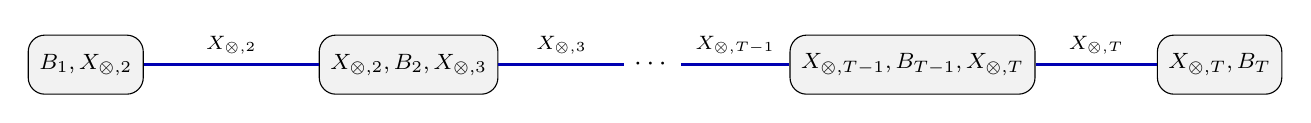
\begin{tikzpicture}[
    clu/.style={draw, fill=gray!10, rounded corners=6pt, inner sep=4pt, minimum height=0.75cm, font=\footnotesize},
    sep/.style={font=\scriptsize, above, text=black, inner sep=3pt},
    flow/.style={very thick, blue!70!black}]
  \node[clu] (d1) at (0, 0)    {$B_1, X_{\otimes,2}$};
  \node[clu] (d2) at (4.1, 0)  {$X_{\otimes,2}, B_2, X_{\otimes,3}$};
  \node      (dots) at (7.2, 0) {$\cdots$};
  \node[clu] (dm) at (10.5, 0) {$X_{\otimes,T-1}, B_{T-1}, X_{\otimes,T}$};
  \node[clu] (dT) at (14.4, 0) {$X_{\otimes,T}, B_T$};
  \draw[flow] (d1) -- node[sep] {$X_{\otimes,2}$} (d2);
  \draw[flow] (d2) -- node[sep] {$X_{\otimes,3}$} (dots);
  \draw[flow] (dots) -- node[sep] {$X_{\otimes,T-1}$} (dm);
  \draw[flow] (dm) -- node[sep] {$X_{\otimes,T}$} (dT);
\end{tikzpicture}
\caption{Graph associated with the local polytope $\mathbb{L}_\otimes$.}
\label{fig:clique-chain}
\end{figure}

\begin{proposition}
\label{prop:exact-marginal}
Up to the change of variables
\[
\mu_{b,1} := \sum_{x'} q_{\mathbf{x}_\otimes,b,x',1}, \qquad q_{x,b,t} := \sum_{x'} q_{x,b,x',t} \ \ \forall t
\in [2:T-1],
\]
the feasible set of the LP~\eqref{eq:LP1} is the local polytope $\mathbb{L}_\otimes$ defined
in~\eqref{eq:local-poly-exact}, i.e., this change of variables is a bijection from $\mathbb{L}_\otimes$ onto the
feasible set of~\eqref{eq:LP1}. Moreover, the local polytope is equal to the marginal polytope, i.e., $\mathbb{L}_\otimes
= \mathbb{M}_\otimes$. Hence the optimal value of~\eqref{eq:LP1} is $J^\star$.
\end{proposition}

\begin{proof}
By the first state constraint~\eqref{eq:local-exact-first}, the only nonzero variables of the first time step are the
$q_{\mathbf{x}_\otimes,b,x',1}$. With the change of variables, the dynamics constraints~\eqref{eq:local-exact-dyn} read $q_{\mathbf{x}_\otimes,b,x',1} =
p_\otimes(x' \mid \mathbf{x}_\otimes, b)\, \mu_{b,1}$ and $q_{x,b,x',t} = p_\otimes(x' \mid x, b)\, q_{x,b,t}$, so
that the marginals are determined by the variables $(\mu, q)$ of~\eqref{eq:LP1}. The normalization constraint~\eqref{eq:local-exact-norm} at $t = 1$
is~\eqref{eq:LP1-first}, and the normalization constraints at $t \ge 2$ follow from it and from the consistency
constraints. By the first state and dynamics constraints, the left-hand side of the consistency
constraint~\eqref{eq:local-exact-cons} is $\sum_{b} p_\otimes(x \mid \mathbf{x}_\otimes, b)\, \mu_{b,1}$ for $t = 1$,
and $\sum_{x',b} p_\otimes(x \mid x', b)\, q_{x',b,t}$ for $t \ge 2$, and its right-hand side is $\sum_b q_{x,b,t+1}$,
so that the consistency constraints are the flow constraints~\eqref{eq:LP1-initial}--\eqref{eq:LP1-flow}. Finally,
the admissibility constraints are the domains of the variables of~\eqref{eq:LP1}. Conversely, the marginals defined from a
feasible $(\mu, q)$ by the expressions above satisfies~\eqref{eq:local-exact-norm}--\eqref{eq:local-exact-cons}, so
that the change of variables is a bijection. We have $\mathbb{M}_\otimes \subseteq \mathbb{L}_\otimes$, and the element of
$\mathbb{M}_\otimes$ given by a Markov policy $\pi$ achieves objective value $J(\pi)$. Conversely, the image $(\mu, q)$
of an element of $\mathbb{L}_\otimes$ is obtained in this way from the policy that draws $B_1$ according to
$\mu_{\cdot,1}$, and $B_t$ according to $\pi_t(b \mid x_{\otimes}) = q_{x_{\otimes},b,t} / \sum_{b^{\prime}}
q_{x_{\otimes},b^{\prime},t}$ at $t \ge 2$ if the denominator is positive (any admissible distribution otherwise), and
its objective value is the cost of this policy.
\end{proof}

\begin{comment}
\begin{proof}
Given a Markov policy $\pi$, $\mu_{b,1} = \mathbb{P}^\pi(B_1 = b)$ and $q_{x_\otimes,b,t} = \mathbb{P}^\pi(X_{\otimes,t}
= x_\otimes, B_t = b)$ satisfy~\eqref{eq:LP1-first}--\eqref{eq:LP1-nonnegative}, so that $\mathbb{M} \subseteq
\mathbb{L}_\otimes$, and the objective value of $(\mu, q)$ is $J(\pi)$.

Conversely, let $(\mu, q) \in \mathbb{L}_\otimes$. We use the junction tree theorem~\cite[Prop.~2.1]{wainwright2008graphical},
which applies to a tree whose nodes are groups of variables and whose edges are labeled by the intersections of the
groups they link, provided that every variable belonging to two nodes belongs to all the nodes of the path between them.
The chain of Figure~\ref{fig:clique-chain} satisfies this property, since $X_{\otimes,t}$ only belongs to two
consecutive nodes and $B_t$ to a single node. We define the distributions of the nodes and of the separators by
\begin{align*}
\tau_1(b, x') &:= \mu_{b,1}\, p_\otimes(x' \mid \mathbf{x}_\otimes, b), &
\tau_t(x, b, x') &:= q_{x,b,t}\, p_\otimes(x' \mid x, b) \quad t \in [2:T-1], \\
\tau_T(x, b) &:= q_{x,b,T}, &
\nu_t(x) &:= \sum_{b \in \mathcal{B}(x)} q_{x,b,t} \quad t \in [2:T].
\end{align*}
They are nonnegative by~\eqref{eq:LP1-nonnegative}. The marginal of $\tau_1$ on $X_{\otimes,2}$ and the marginal of
$\tau_{t-1}$ on $X_{\otimes,t}$ are equal to $\nu_2$ and $\nu_t$ by~\eqref{eq:LP1-initial} and~\eqref{eq:LP1-flow}
respectively, and the marginal of $\tau_t$ and of $\tau_T$ on $X_{\otimes,t}$ is $\nu_t$ by definition. Since $\tau_1$
sums to $1$ by~\eqref{eq:LP1-first}, all these distributions sum to $1$ by induction on $t$. The normalization and
marginalization conditions~\cite[Eq.~(2.13)]{wainwright2008graphical} hold, so that by the junction tree theorem the
$\tau_t$ are the marginals of the distribution~\cite[Eq.~(2.12)]{wainwright2008graphical}
\[
P(b_1, x_2, b_2, \dots, x_T, b_T) := \tau_1(b_1, x_2) \prod_{t=2}^{T-1} \frac{\tau_t(x_t, b_t, x_{t+1})}{\nu_t(x_t)}\
\frac{\tau_T(x_T, b_T)}{\nu_T(x_T)},
\]
with the convention $0/0 = 0$. Let $\pi$ be the Markov policy that draws $B_1$ according to $\mu_{\cdot,1}$, and $B_t$
according to $\pi_t(b \mid x) := q_{x,b,t} / \nu_t(x)$ at $t \ge 2$ if $\nu_t(x) > 0$, and according to any distribution
on $\mathcal{B}(x)$ otherwise. It is admissible since $q_{x,b,t}$ is only defined for $b \in \mathcal{B}(x)$.
For every trajectory such that $\nu_t(x_t) > 0$ for all $t \in [2:T]$, substituting the definitions of the $\tau_t$
gives
\[
P(b_1, x_2, \dots, b_T) = \mu_{b_1,1}\, p_\otimes(x_2 \mid \mathbf{x}_\otimes, b_1) \prod_{t=2}^{T-1} \pi_t(b_t \mid x_t)\,
p_\otimes(x_{t+1} \mid x_t, b_t)\ \pi_T(b_T \mid x_T),
\]
whose right-hand side is the probability $P^\pi(b_1, x_2, \dots, b_T)$ of the trajectory under $\pi$. Since $P$ vanishes
on the other trajectories and sums to $1$, $P^\pi$ sums to $1$ on these trajectories, hence vanishes on the other ones,
and $P = P^\pi$. Hence
$\mu_{b,1} = \mathbb{P}^\pi(B_1 = b)$ and $q_{x,b,t} = \tau_t$ marginalized on $(X_{\otimes,t}, B_t)$, i.e., $q_{x,b,t} =
\mathbb{P}^\pi(X_{\otimes,t} = x, B_t = b)$, so that $(\mu, q) \in \mathbb{M}$, and the objective value of $(\mu, q)$ is
$J(\pi)$. Therefore $\mathbb{L}_\otimes = \mathbb{M}$, and the optimal value of~\eqref{eq:LP1} is the minimum of $J(\pi)$
over Markov policies, i.e., $J^\star$.
\end{proof}
\end{comment}

In general, the marginal polytope is strictly included in the local polytope. We will see in
Section~\ref{sec:why-gap} that the equality $\mathbb{L}_\otimes = \mathbb{M}_\otimes$ obtained here is explained by the
structure of the graph of Figure~\ref{fig:clique-chain}.
Note that the variables of the local polytope are the distributions of the subsets of
variables whose joint distribution is known. In the LP, the variables are the parts of these distributions that are
degrees of freedom. The exact LP is intractable because its subsets contain the joint state
and the joint action, so that its number of variables is proportional to the number of joint
states and to the number of joint actions, which are both too large to be enumerated explicitly. In what follows we explain how to build
tractable approximations following the same 
methodology, with smaller subsets of variables. 


\subsection{Joint fluid LP}
\label{sec:full-fluid}
Our first approximation is built in the same way as the classical fluid approximations of D-MDPs, whose variables are
local distributions. This removes the first of the two difficulties of the exact LP~\eqref{eq:LP1}, namely that its
number of variables grows with the size of the joint state space. The number of variables of our LP still grows with
the size of the joint action space, but we show that this second difficulty can be handled by column
generation~\cite{desrosiers2005primer}. Column generation is efficient in
practice as soon as the pricing problem can be solved efficiently. We show that the pricing problem, which consists in
finding a maintenance schedule of minimum reduced cost, can be reformulated as a small MILP.

\paragraph{Subsets of variables and sufficient statistics.} In the fluid approximation of D-MDPs of Bertsimas and
Mišić~\cite{bertsimas2016}, the variables are the probabilities of the local states and local actions of the
subsystems, and the probabilities of the global actions. Compared with the exact LP, we therefore replace the subsets
$(X_{\otimes,t}, B_t, X_{\otimes,t+1})$ of the joint states by two types of smaller subsets, the \emph{local subsets}
of every component $m$ and the \emph{joint action subsets} $B_t$, and keep the indicators of their values as
sufficient statistics (Table~\ref{tab:subsets-joint}). The associated graph is represented in Figure~\ref{fig:non-tree-graph}.

\begin{table}[h]
\centering
\small
\renewcommand{\arraystretch}{1.3}
\begin{tabular}{|l|l|l|}
\hline
Subset & Sufficient statistics & Marginals \\
\hline
$(X_{m,t}, A_{m,t}, X_{m,t+1})$, $t \in [1:T-1]$ & $\mathds{1}_{\{X_{m,t} = x,\, A_{m,t} = a,\, X_{m,t+1} = x'\}}$,
$x, x' \in \mathcal{X}_m$, $a \in \mathcal{A}_m(x)$ & $q^m_{x,a,x',t}$ \\
$(X_{m,T}, A_{m,T})$ & $\mathds{1}_{\{X_{m,T} = x,\, A_{m,T} = a\}}$, $x \in \mathcal{X}_m$, $a \in \mathcal{A}_m(x)$ &
$q^m_{x,a,T}$ \\
$B_1$ & $\mathds{1}_{\{B_1 = b\}}$, $b \in \mathcal{B}(\mathbf{x}_\otimes)$ & $\mu_{b,1}$ \\
$B_t$, $t \in [2:T]$ & $\mathds{1}_{\{B_t = b\}}$, $b \in \mathcal{B}$ & $\mu_{b,t}$ \\
\hline
\end{tabular}
\caption{Subsets of variables, sufficient statistics and marginals of the Joint fluid LP, for every component $m \in
[M]$.}
\label{tab:subsets-joint}
\end{table}

\begin{figure}[h]
\centering
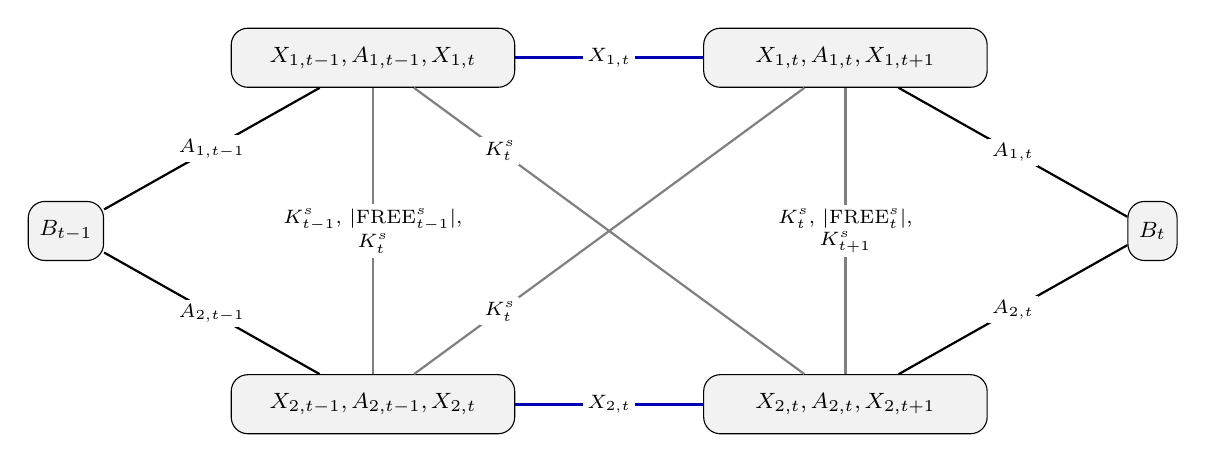
\begin{tikzpicture}[
    clu/.style={draw, fill=gray!10, rounded corners=6pt, inner sep=4pt, minimum height=0.75cm, font=\footnotesize},
    sub/.style={clu, minimum width=3.6cm},
    sep/.style={font=\scriptsize, fill=white, text=black, inner sep=1.5pt, align=center},
    flow/.style={very thick, blue!70!black},
    cons/.style={thick},
    quota/.style={thick, gray}]
  \node[sub] (d1a) at (0, 2.2)    {$X_{1,t-1}, A_{1,t-1}, X_{1,t}$};
  \node[sub] (d2a) at (0, -2.2)   {$X_{2,t-1}, A_{2,t-1}, X_{2,t}$};
  \node[clu] (ba)  at (-3.9, 0)   {$B_{t-1}$};
  \node[sub] (d1b) at (6, 2.2)    {$X_{1,t}, A_{1,t}, X_{1,t+1}$};
  \node[sub] (d2b) at (6, -2.2)   {$X_{2,t}, A_{2,t}, X_{2,t+1}$};
  \node[clu] (bb)  at (9.9, 0)    {$B_t$};
  % quota consistency between the two components (drawn first, so that the other edges are on top)
  \draw[quota] (d1a) -- node[sep, pos=0.22] {$K^s_t$} (d2b);
  \draw[quota] (d2a) -- node[sep, pos=0.22] {$K^s_t$} (d1b);
  \draw[quota] (d1a) -- node[sep] {$K^s_{t-1}$, $|\text{FREE}^s_{t-1}|$,\\$K^s_t$} (d2a);
  \draw[quota] (d1b) -- node[sep] {$K^s_t$, $|\text{FREE}^s_t|$,\\$K^s_{t+1}$} (d2b);
  % local flow constraints
  \draw[flow] (d1a) -- node[sep] {$X_{1,t}$} (d1b);
  \draw[flow] (d2a) -- node[sep] {$X_{2,t}$} (d2b);
  % consistency with the joint action
  \draw[cons] (ba) -- node[sep] {$A_{1,t-1}$} (d1a);
  \draw[cons] (ba) -- node[sep] {$A_{2,t-1}$} (d2a);
  \draw[cons] (bb) -- node[sep] {$A_{1,t}$} (d1b);
  \draw[cons] (bb) -- node[sep] {$A_{2,t}$} (d2b);
\end{tikzpicture}
\caption{Graph associated with the local polytope $\mathbb{L}^{\mathrm{J}}$, for two components of the same
substation $s$. }
\label{fig:non-tree-graph}
\end{figure}

\paragraph{Marginal polytope.}
\label{sec:marginal-local}
The values of the marginals that can be obtained from a Markov policy form the \emph{fluid
marginal polytope}
\begin{equation}
\label{eq:local-marg-poly}
\begin{aligned}
\mathbb{M}^{\mathrm{J}} := \Big\{ (\mu, q) \ \Big|\ \exists \pi \text{ Markov policy},\
& \mu_{b,1} = \mathbb{P}^\pi(B_1 = b) \quad \forall b \in \mathcal{B}(\mathbf{x}_\otimes), \\
& \mu_{b,t} = \mathbb{P}^\pi(B_t = b) \quad \forall b \in \mathcal{B},\ t \in [2:T], \\
& q^m_{x,a,x',t} = \mathbb{P}^\pi\big(X_{m,t} = x,\, A_{m,t} = a,\, X_{m,t+1} = x'\big) \\
& \qquad \forall m \in [M],\ x, x' \in \mathcal{X}_m,\ a \in \mathcal{A}_m(x),\ t \in [1:T-1], \\
& q^m_{x,a,T} = \mathbb{P}^\pi\big(X_{m,T} = x,\, A_{m,T} = a\big) \\
& \qquad \forall m \in [M],\ x \in \mathcal{X}_m,\ a \in \mathcal{A}_m(x) \Big\}.
\end{aligned}
\end{equation}

\paragraph{Cost approximation.}
\label{sec:intro-approx}
We want to solve an LP whose variables are the marginals associated with the sufficient statistics above. Its
objective should express, or approximate, the expected cost as a linear combination of these variables. Since the marginals are here
probabilities, this holds for any cost approximation that decomposes over the subsets, i.e., is a sum of terms that each depend on
the variables of a single subset. At the first time step, the true cost $c_\otimes(\mathbf{x}_\otimes, b)$ only depends on $B_1$, and
its expectation is linear in $\mu_{\cdot,1}$. At $t \ge 2$, the true cost does not have this form, since the
penalty~\eqref{eq:intro-penalty} depends jointly on the degradation states of the components of a substation. We
therefore replace it by a separable approximation. We define the \emph{maintenance cost} and the \emph{failure cost} of
component $m$
\begin{align}
c^{\mathrm{maint}} \ &:=\ \sum_{s} \sum_{\tau \notin \text{Free}^s} m^s_\tau,
\label{eq:intro-maintenance-cost}\\
c^{\mathrm{fail}}_m \ &:=\ \big(60 - \kappa_m\big)\, \ell_m(n_m),
\label{eq:intro-failure-cost}
\end{align}
and the \emph{local cost} $c^{\mathrm{loc}}_m := \delta_m c^{\mathrm{rep}}_m + c^{\mathrm{fail}}_m$. We write $\tilde c_m(x, a) :=
c^{\mathrm{loc}}_m$, which only depends on the local state and the local action of component $m$, and $f(b) :=
c^{\mathrm{maint}}$, the \emph{joint action cost}, which only depends on $b$. The approximation of the cost is
\begin{equation}
\label{eq:cost_approx}
\tilde c_\otimes(x_\otimes,b) = \sum_{m \in [M]} \tilde c_m\big(x, A_m(b)\big) + f(b).
\end{equation}
This approximation is moreover an upper bound of the true cost,
\begin{equation}
\label{eq:intro-cost-approx}
c^{\mathrm{tot}} \ \le\ \sum_{m \in [M]} c^{\mathrm{loc}}_m \ +\ c^{\mathrm{maint}},
\end{equation}
since it mainly replaces the maximum of the nonnegative losses of the components of a substation by their sum
(Appendix~\ref{app:cost-bound}). The bound is tight when no component of the substation is maintained and at most
one of its components is degraded. Since components of offshore substations are chosen for their high reliability,
simultaneous degradations are rare, and we prefer an overestimation of the penalties to an underestimation, given
their high cost.

The expectation of the approximation~\eqref{eq:cost_approx} at $t \ge 2$ is a linear function of the marginals of the
subsets. Indeed, by linearity of the expectation, and since each term only depends on the variables of a single subset,
\begin{equation}
\label{eq:cost_approx_expectation}
\begin{aligned}
\mathbb{E}\big[\tilde c_\otimes(X_{\otimes,t}, B_t)\big]
&= \sum_{m \in [M]} \mathbb{E}\big[\tilde c_m(X_{m,t}, A_{m,t})\big] + \mathbb{E}\big[f(B_t)\big] \\
&= \sum_{m \in [M]} \sum_{x, a} \tilde c_m(x, a)\, \mathbb{P}\big(X_{m,t} = x,\, A_{m,t} = a\big)
+ \sum_{b \in \mathcal{B}} f(b)\, \mathbb{P}(B_t = b) \\
&= \sum_{m \in [M]} \sum_{x, a} \tilde c_m(x, a) \sum_{x'} q^m_{x,a,x',t} + \sum_{b \in \mathcal{B}} f(b)\,
\mu_{b,t}
\end{aligned}
\end{equation}
for $t \in [2:T-1]$, and the same expression with $q^m_{x,a,T}$ in place of $\sum_{x'} q^m_{x,a,x',t}$ at
$t = T$.

\paragraph{Local polytope.} The local polytope $\mathbb{L}^{\mathrm{J}}$ is defined by the constraints of
Section~\ref{sec:marginal-polytopes} for the subsets above. The variables are only defined for admissible actions,
$a \in \mathcal{A}_m(x)$ and $b \in \mathcal{B}(\mathbf{x}_\otimes)$ at $t = 1$, which gives the admissibility
constraints, and in particular the quota constraint~\eqref{eq:intro-quota-constraint}. The normalization constraints
are
\begin{subequations}
\label{eq:fluid-local-norm}
\begin{align}
& \sum_{b \in \mathcal{B}(\mathbf{x}_\otimes)} \mu_{b,1} = 1, \qquad \sum_{b \in \mathcal{B}} \mu_{b,t} = 1
\quad \forall t \in [2:T], \\
& \sum_{x \in \mathcal{X}_m} \sum_{a \in \mathcal{A}_m(x)} \sum_{x' \in \mathcal{X}_m} q^m_{x,a,x',t} = 1
\quad \forall m \in [M],\ t \in [1:T-1], \\
& \sum_{x \in \mathcal{X}_m} \sum_{a \in \mathcal{A}_m(x)} q^m_{x,a,T} = 1 \quad \forall m \in [M].
\end{align}
\end{subequations}
Since the local state of component $m$ at $t = 1$ is $\mathbf{x}_m$, the first state constraints are
\begin{equation}
\label{eq:fluid-local-first}
q^m_{x,a,x',1} = 0 \qquad \forall m \in [M],\ x \in \mathcal{X}_m \setminus \{\mathbf{x}_m\},\ a \in
\mathcal{A}_m(x),\ x' \in \mathcal{X}_m.
\end{equation}
Since no subset contains the joint state, we have no marginals on the joint states, and we cannot impose the joint
dynamics. However, we can impose the local dynamics through dynamics constraints on the marginals of the subsets
$(X_{m,t}, A_{m,t}, X_{m,t+1})$,
\begin{equation}
\label{eq:fluid-local-dyn}
\begin{aligned}
& q^m_{x,a,x',t} = p_m(x' \mid x, a) \sum_{x'' \in \mathcal{X}_m} q^m_{x,a,x'',t} \\
& \qquad \forall m \in [M],\ x, x' \in \mathcal{X}_m,\ a \in \mathcal{A}_m(x),\ t \in [1:T-1].
\end{aligned}
\end{equation}
The graph of the subsets is represented in Figure~\ref{fig:non-tree-graph}, and gives three types of consistency
constraints. The edges labeled $X_{m,t+1}$ (blue) state that two consecutive subsets of component $m$ give the same law
of $X_{m,t+1}$,
\begin{subequations}
\label{eq:fluid-local-cons-x}
\begin{align}
& \sum_{x' \in \mathcal{X}_m} \sum_{a \in \mathcal{A}_m(x')} q^m_{x',a,x,t} = \sum_{a \in \mathcal{A}_m(x)}
\sum_{x'' \in \mathcal{X}_m} q^m_{x,a,x'',t+1} \quad \forall m \in [M],\ x \in \mathcal{X}_m,\ t \in [1:T-2], \\
& \sum_{x' \in \mathcal{X}_m} \sum_{a \in \mathcal{A}_m(x')} q^m_{x',a,x,T-1} = \sum_{a \in \mathcal{A}_m(x)}
q^m_{x,a,T} \quad \forall m \in [M],\ x \in \mathcal{X}_m.
\end{align}
\end{subequations}
The edges labeled $A_{m,t}$ (black) state that the subset of component $m$ and the subset $B_t$ give the same law of
$A_{m,t}$,
\begin{subequations}
\label{eq:fluid-local-cons-a}
\begin{align}
& \sum_{x \in \mathcal{X}_m \mid a \in \mathcal{A}_m(x)} \sum_{x' \in \mathcal{X}_m} q^m_{x,a,x',t} = \sum_{b \mid A_m(b) = a} \mu_{b,t}
\quad \forall m \in [M],\ a \in \mathcal{A}_m,\ t \in [1:T-1], \\
& \sum_{x \in \mathcal{X}_m \mid a \in \mathcal{A}_m(x)} q^m_{x,a,T} = \sum_{b \mid A_m(b) = a} \mu_{b,T} \quad \forall m \in [M],\ a \in
\mathcal{A}_m.
\end{align}
\end{subequations}
The edges (gray) between the subsets at $t$ of two components $m, m' \in \mathcal{M}^s$ of the same substation state
that they give the same law of their shared quota variables $(K^s_t, |\text{FREE}^s_t|, K^s_{t+1})$,
\begin{subequations}
\label{eq:fluid-local-cons-q}
\begin{align}
& \sum_{n, \delta, n'} q^m_{(n,k),(\delta,\kappa),(n',k'),t} = \sum_{n, \delta, n'}
q^{m'}_{(n,k),(\delta,\kappa),(n',k'),t} \quad \forall s \in [S],\ m, m' \in \mathcal{M}^s\!,\ k, \kappa, k' \in
[0:K_0],\ t \in [1:T-1], \\
& \sum_{n, \delta} q^m_{(n,k),(\delta,\kappa),T} = \sum_{n, \delta} q^{m'}_{(n,k),(\delta,\kappa),T} \quad
\forall s \in [S],\ m, m' \in \mathcal{M}^s\!,\ k, \kappa \in [0:K_0].
\end{align}
\end{subequations}
The diagonal edges labeled $K^s_t$ give constraints that follow from~\eqref{eq:fluid-local-cons-x}
and~\eqref{eq:fluid-local-cons-q}, so that we do not write them. The local polytope is then
\begin{equation}
\label{eq:fluid-local-poly}
\mathbb{L}^{\mathrm{J}} := \Big\{ (\mu, q) \ge 0 \ \Big|\ (\mu, q) \text{
satisfies}~\eqref{eq:fluid-local-norm}\text{--}\eqref{eq:fluid-local-cons-q} \Big\}.
\end{equation}
Since these constraints are necessary, $\mathbb{M}^{\mathrm{J}} \subseteq \mathbb{L}^{\mathrm{J}}$.

\paragraph{Joint fluid LP.} We consider the following LP:
\begin{subequations}\label{eq:fluid}
\begin{align}
\min_{q,\mu} \quad
& \sum_{b \in \mathcal{B}(\mathbf{x}_\otimes)} c_\otimes(\mathbf{x}_\otimes, b)\, \mu_{b,1}
\nonumber\\
& \ +\ \sum_{t=2}^{T} \Bigg( \sum_{m,\, x,\, a} \tilde c_m(x,a)\, q^m_{x,a,t}
+ \sum_{b \in \mathcal{B}} f(b)\, \mu_{b,t} \Bigg)
\label{eq:fluid-obj}\\
\text{s.t.} \quad
& \sum_{b \in \mathcal{B}(\mathbf{x}_\otimes)} \mu_{b,1} = 1
\label{eq:fluid-first}\\
& \sum_{a \in \mathcal{A}_m(x)} q^m_{x,a,2} = \sum_{b \in \mathcal{B}(\mathbf{x}_\otimes)} p_m\big(x \mid
\mathbf{x}_m, A_m(b)\big)\, \mu_{b,1}
&& \forall m \in [M], x \in \mathcal{X}_m
\label{eq:fluid-initial}\\
& \sum_{a \in \mathcal{A}_m(x)} q^m_{x,a,t}
= \sum_{x',\, a} p_m(x \mid x',a)\, q^m_{x',a,t-1}
&& \forall m \in [M], x \in \mathcal{X}_m, t \in [3:T]
\label{eq:fluid-flow}\\
& \sum_{x \in \mathcal{X}_m \mid a \in \mathcal{A}_m(x)} q^m_{x,a,t}
= \sum_{b \in \mathcal{B} \mid A_m(b)=a} \mu_{b,t}
&& \forall m \in [M], a \in \mathcal{A}_m, t \in [2:T]
\label{eq:fluid-consistency}\\
& \sum_{n, \delta} q^m_{(n,k),(\delta,\kappa),t} = \sum_{n, \delta} q^{m'}_{(n,k),(\delta,\kappa),t}
&& \forall s \in [S], m, m' \in \mathcal{M}^s\!, k, \kappa \in [0:K_0], t \in [2:T]
\label{eq:fluid-copies}\\
& q^m_{x,a,t} \geq 0
&& \forall m \in [M], x \in \mathcal{X}_m, a \in \mathcal{A}_m(x), t \in [2:T]
\nonumber\\
& \mu_{b,1} \geq 0 \quad \forall b \in \mathcal{B}(\mathbf{x}_\otimes), \qquad \mu_{b,t} \geq 0
&& \forall b \in \mathcal{B}, t \in [2:T].
\label{eq:fluid-nonneg}
\end{align}
\end{subequations}
In~\eqref{eq:fluid}, the variable $q^m_{(n,k),(\delta,\kappa),t}$ is only defined for $\kappa \le k$. Note that the cost
is only approximated at $t \ge 2$: since the first state is known, it is possible to represent the exact cost at first stage without
representing the distribution of the joint state. The proposition that follows show that the feasible set 
of~\eqref{eq:fluid} is (up to a change of variables) the local polytope $\mathbb{L}^{\mathrm{J}}$.

\begin{proposition}
\label{prop:fluid-relaxation}
Up to the change of variables
\begin{equation}
\label{eq:fluid-change}
q^m_{x,a,t} := \sum_{x'} q^m_{x,a,x',t} \quad \forall t \in [2:T-1],
\end{equation}
the feasible set of~\eqref{eq:fluid} is exactly the local polytope $\mathbb{L}^{\mathrm{J}}$. Hence it contains
$\mathbb{M}^{\mathrm{J}}$.
\end{proposition}

\begin{proof}
The proof follows that of Proposition~\ref{prop:exact-marginal}. For $t \ge 2$, the dynamics
constraints~\eqref{eq:fluid-local-dyn} give $q^m_{x,a,x',t} = p_m(x' \mid x, a)\, q^m_{x,a,t}$, the admissibility constraints are the domains of the
variables, the normalization constraint of $B_1$ is~\eqref{eq:fluid-first}, the normalization constraints at $t \ge 2$
are redundant, the consistency constraints~\eqref{eq:fluid-local-cons-x} are the flow
constraints~\eqref{eq:fluid-initial}--\eqref{eq:fluid-flow}, and the converse gives the bijection, as in this proof.
Two points are new. First, there is no variable $q^m$ at $t = 1$, and the first state, dynamics and consistency
constraints~\eqref{eq:fluid-local-cons-a} with $B_1$ give $q^m_{x,a,x',1} = \mathds{1}_{\{x = \mathbf{x}_m\}}\,
p_m(x' \mid \mathbf{x}_m, a) \sum_{b \mid A_m(b) = a} \mu_{b,1}$. Second, $\mathbb{L}^{\mathrm{J}}$ contains
consistency constraints with the joint action and between the components. The consistency
constraints~\eqref{eq:fluid-local-cons-a} at $t \ge 2$ are~\eqref{eq:fluid-consistency}. Since $K^s_{t+1} =
\phi_t(K^s_t, |\text{FREE}^s_t|)$, the consistency constraints~\eqref{eq:fluid-local-cons-q} at $t \ge 2$
are~\eqref{eq:fluid-copies}, and at $t = 1$ they are redundant, since both sides are the law of $(\mathbf{k}^s,
\kappa^s(B_1), \phi_1(\mathbf{k}^s, \kappa^s(B_1)))$ under $\mu_{\cdot,1}$.
\end{proof}

\begin{remark}
Proposition~\ref{prop:fluid-relaxation} does not imply $Z \le J^\star$, because of the cost approximation. 
\end{remark}

\paragraph{Column generation.}
\label{sec:column-generation}
The variables $\mu_{b,t}$ are indexed by $\mathcal{B}(\mathbf{x}_\otimes)$ at $t = 1$ and by $\mathcal{B}$ at $t \ge
2$, which cannot be enumerated. We generate them by column generation~\cite{desrosiers2005primer}, at every time
step: we solve a restricted master problem (RMP) over subsets $\mathcal{B}'_1 \subseteq \mathcal{B}(\mathbf{x}_\otimes)$ and
$\mathcal{B}'_t \subseteq \mathcal{B}$, $t \ge 2$. We write $\eta$ for the dual variable of~\eqref{eq:fluid-first},
$\nu^m_{x}$ for the dual variable of~\eqref{eq:fluid-initial} for $m$ and $x$, and $\lambda^{m,a}_t$ for the dual
variable of~\eqref{eq:fluid-consistency} for $m$, $a$ and $t$, with signs chosen so that the reduced costs of the
columns are
\[
\overline{c}(b,1) = c_\otimes(\mathbf{x}_\otimes, b) + \sum_{m \in [M]} \sum_{x \in \mathcal{X}_m} \nu^m_{x}\,
p_m\big(x \mid \mathbf{x}_m, A_m(b)\big) - \eta,
\qquad
\overline{c}(b,t) = f(b) + \sum_{m \in [M]} \lambda^{m,A_m(b)}_t \quad (t \ge 2).
\]
The RMP solution is optimal for~\eqref{eq:fluid} if no column has a negative reduced cost. Finding the column of most
negative reduced cost amounts to solving, at the first time step, the \emph{first-step pricing problem}
\begin{equation}\label{eq:pricing-first}
  \min_{b \in \mathcal{B}(\mathbf{x}_\otimes)} \left[ c_\otimes(\mathbf{x}_\otimes, b) + \sum_{m \in [M]} \sum_{x \in
  \mathcal{X}_m} \nu^m_{x}\, p_m\big(x \mid \mathbf{x}_m, A_m(b)\big) \right],
\end{equation}
and, at every time step $t \ge 2$, the \emph{pricing problem}
\begin{equation}\label{eq:pricing}
  \min_{b \in \mathcal{B}} \left[ f(b) + \sum_{m \in [M]} \lambda^{m,A_m(b)}_t \right].
\end{equation}
Both pricing problems can be written as MILPs, by encoding a joint action with binary variables. Three terms need
to be linearized, the maintenance indicator $m^s_\tau$, which is a maximum over the components of the substation, the
products of $m^s_\tau$ and of the indicator that day $\tau$ is a declared day in the joint action cost $f$, and
the dual terms, which depend on the local actions. We encode the start days, the repairs and the declared days with binary indicators, and replace the maximum and the products by continuous variables bounded by these indicators.
The number of declared days of substation $s$ is encoded by the binary indicators
$\chi^s_\kappa$, $\kappa \in [0:K_0]$, equal to $1$ if $s$ declares $\kappa$ days. A
joint action is then encoded by the vector $b$ of all these variables, on which $f(b)$ and $c_\otimes(\mathbf{x}_\otimes, b)$ are linear. The
complete MILPs are given in Appendix~\ref{app:maintenance-problem}.

\begin{algorithm}[H]
\caption{Column generation for the Joint fluid LP~\eqref{eq:fluid}}
\label{alg:column-generation}
\begin{algorithmic}[1]
\State Initialize $\mathcal{B}'_1 \subseteq \mathcal{B}(\mathbf{x}_\otimes)$ and $\mathcal{B}'_t \subseteq \mathcal{B}$ for $t \in [2:T]$
\Repeat
    \State Solve the RMP over $(\mathcal{B}'_t)_{t \in [T]}$ and retrieve the duals $\eta$, $\nu^m_{x}$ and $\lambda^{m,a}_t$
    \For{$t = 1, \ldots, T$}
        \State Solve the pricing problem~\eqref{eq:pricing-first} (if $t = 1$) or~\eqref{eq:pricing} (if $t \ge 2$) to obtain $b^\star$ and $\overline{c}(b^\star,t)$
        \If{$\overline{c}(b^\star,t) < 0$}
            \State $\mathcal{B}'_t \gets \mathcal{B}'_t \cup \{b^\star\}$
        \EndIf
    \EndFor
\Until{no improving column is found or the iteration limit is reached}
\end{algorithmic}
\end{algorithm}

The tractability of the Joint fluid LP comes from the structure of the MDP, which allows us to build convenient subsets
of variables. More precisely, since the dynamics of a component only depend on its local action, we put the local
action, and not the joint action, in the subsets of the component. The only variables shared by the subsets of the
components and the subsets $B_t$ are thus the local actions, which take their values in a small set. The consistency
constraints~\eqref{eq:fluid-consistency} between these subsets can therefore be written for each value of the local
action, which gives a polynomial number of constraints. Only the number of variables is large, and not the number of
constraints, which makes column generation possible.

\subsection{Compact fluid LP}
\label{sec:compact}

In the classical fluid approximations of W-MDPs~\cite{AdelmanMersereau2008}, the variables are the probabilities of the
local states and local actions, and the constraints that couple the local actions are only imposed in expectation.
Since these constraints are linear in the local actions, this amounts to imposing them on the mean values of the local
actions. We show that the same
approach applies to our problem. It gives a formulation that can be solved directly, without column generation, but
whose approximation is a priori looser than that of the Joint fluid LP.

\paragraph{Subsets of variables and sufficient statistics.} Compared with the Joint fluid LP, the Compact fluid LP
keeps the same subsets and only changes the sufficient statistic of the joint action subsets $B_t$, at every time step
including the first one (Table~\ref{tab:subsets-compact}). The sufficient statistic of $B_t$ is the vector $B_t$
itself, that is the vector of the variables of the MILP encoding of the joint actions
(Section~\ref{sec:column-generation}), and its marginal is the vector $\bar b_t := \mathbb{E}[B_t]$ of the means of
these variables.

\begin{table}[h]
\centering
\small
\renewcommand{\arraystretch}{1.3}
\begin{tabular}{|l|l|l|}
\hline
Subset & Sufficient statistics & Marginals \\
\hline
$(X_{m,t}, A_{m,t}, X_{m,t+1})$, $t \in [1:T-1]$ & $\mathds{1}_{\{X_{m,t} = x,\, A_{m,t} = a,\, X_{m,t+1} = x'\}}$,
$x, x' \in \mathcal{X}_m$, $a \in \mathcal{A}_m(x)$ & $q^m_{x,a,x',t}$ \\
$(X_{m,T}, A_{m,T})$ & $\mathds{1}_{\{X_{m,T} = x,\, A_{m,T} = a\}}$, $x \in \mathcal{X}_m$, $a \in \mathcal{A}_m(x)$ &
$q^m_{x,a,T}$ \\
$B_t$, $t \in [T]$ & $B_t$ & $\bar b_t$ \\
\hline
\end{tabular}
\caption{Subsets of variables, sufficient statistics and marginals of the Compact fluid LP, for every component $m
\in [M]$. Only the last row differs from Table~\ref{tab:subsets-joint}.}
\label{tab:subsets-compact}
\end{table}

\paragraph{Marginal polytope.} The values of these marginals that can be obtained from a Markov policy form the polytope
\begin{equation}
\label{eq:compact-marg-poly}
\begin{aligned}
\mathbb{M}^{\mathrm{C}} := \Big\{ (q, \bar b) \ \Big|\ & \exists \pi \text{ Markov policy},\ \forall m, x,
a, x', t,\ \ \bar b_t = \mathbb{E}^\pi[B_t], \\
& q^m_{x,a,x',t} = \mathbb{P}^\pi\big(X_{m,t} = x,\, A_{m,t} = a,\, X_{m,t+1} = x'\big), \\
& q^m_{x,a,T} = \mathbb{P}^\pi\big(X_{m,T} = x,\, A_{m,T} = a\big) \Big\}.
\end{aligned}
\end{equation}
This set has too many facets to admit a tractable description.

\paragraph{Local polytope.} The local polytope $\mathbb{L}^{\mathrm{C}}$ is built as $\mathbb{L}^{\mathrm{J}}$
in Section~\ref{sec:full-fluid}, and only the constraints that involve the subsets $B_t$ change. The first state
constraints~\eqref{eq:fluid-local-first} and the dynamics constraints~\eqref{eq:fluid-local-dyn} are the same, as well
as the normalization constraints of the local subsets. There is no normalization constraint for the subsets $B_t$,
since their marginals are means and not probability distributions. We write $\bar{\mathcal{B}}$ and
$\bar{\mathcal{B}}(\mathbf{x}_\otimes)$ the polytopes obtained from the encodings of $\mathcal{B}$ and
$\mathcal{B}(\mathbf{x}_\otimes)$ by relaxing every binary variable into $[0,1]$, and extend $\delta_m$, $\chi^s_\kappa$, $f$
and $c_\otimes(\mathbf{x}_\otimes, \cdot)$ to them linearly. The marginal $\bar b_t$ lies in $\mathrm{conv}(\mathcal{B})
\subseteq \bar{\mathcal{B}}$ for $t \ge 2$, and in $\mathrm{conv}(\mathcal{B}(\mathbf{x}_\otimes)) \subseteq
\bar{\mathcal{B}}(\mathbf{x}_\otimes)$ for $t = 1$. The admissibility constraints of the subsets $B_t$ only impose that
these means belong to the relaxed polytopes,
\begin{equation}
\label{eq:compact-local-adm}
\bar b_1 \in \bar{\mathcal{B}}(\mathbf{x}_\otimes), \qquad \bar b_t \in \bar{\mathcal{B}} \quad \forall t \in [2:T].
\end{equation}
The constraint~\eqref{eq:compact-local-adm} that $\bar b_t$ belongs to $\bar{\mathcal{B}}$ is the analogue of the
normalization constraint when the marginals are means and not probability distributions. In particular, we do not impose that $\bar b_t$ is the mean of a distribution over admissible joint actions, that is,
that it belongs to $\mathrm{conv}(\mathcal{B})$, or to $\mathrm{conv}(\mathcal{B}(\mathbf{x}_\otimes))$ at $t = 1$. The
consistency constraints between consecutive subsets of a component~\eqref{eq:fluid-local-cons-x} and between the
components of a same substation~\eqref{eq:fluid-local-cons-q} are the same. Only the consistency constraints between
the subsets $B_t$ and the local subsets change, since the marginal of $B_t$ is now its mean. The joint action $B_t$
contains the binary variables $\delta_m$ and $\chi^s_\kappa$ of the MILP encoding. The means of the binary variables 
can be interpreted as probabilities. For instance,
$\delta_m(\bar b_t)$ is the probability that component $m$ is maintained at $t$, and $\chi^s_\kappa(\bar b_t)$ the
probability that substation $s$ declares $\kappa$ days. The mean $\bar b_t$ thus gives the distribution of
$\Delta_{m,t}$ and the distribution of $|\text{FREE}^{s(m)}_t|$, but not their joint distribution. The consistency
constraints are as follows:
\begin{subequations}
\label{eq:compact-local-cons-a}
\begin{align}
& \sum_{\kappa} \sum_{x \in \mathcal{X}_m \mid (1,\kappa) \in \mathcal{A}_m(x)} \sum_{x' \in \mathcal{X}_m}
q^m_{x,(1,\kappa),x',t} = \delta_m(\bar b_t), \nonumber \\
& \sum_{\delta} \sum_{x \in \mathcal{X}_m \mid (\delta,\kappa) \in \mathcal{A}_m(x)} \sum_{x' \in \mathcal{X}_m}
q^m_{x,(\delta,\kappa),x',t} = \chi^{s(m)}_\kappa(\bar b_t) \nonumber \\
& \qquad \forall m \in [M],\ \kappa \in [0:K_0],\ t \in [1:T-1], \\
& \sum_{\kappa} \sum_{x \in \mathcal{X}_m \mid (1,\kappa) \in \mathcal{A}_m(x)} q^m_{x,(1,\kappa),T} =
\delta_m(\bar b_T), \qquad
\sum_{\delta} \sum_{x \in \mathcal{X}_m \mid (\delta,\kappa) \in \mathcal{A}_m(x)} q^m_{x,(\delta,\kappa),T} =
\chi^{s(m)}_\kappa(\bar b_T)
\nonumber \\
& \qquad \forall m \in [M],\ \kappa \in [0:K_0].
\end{align}
\end{subequations}
They replace the consistency constraints~\eqref{eq:fluid-local-cons-a} of $\mathbb{L}^{\mathrm{J}}$.

\paragraph{Cost approximation.} At $t \ge 2$, we use the same separable approximation as in
Section~\ref{sec:full-fluid}. Since $f$ and $c_\otimes(\mathbf{x}_\otimes, \cdot)$ are linear,
$\mathbb{E}[f(B_t)] = f(\mathbb{E}[B_t]) = f(\bar b_t)$, and $\mathbb{E}[c_\otimes(\mathbf{x}_\otimes, B_1)] =
c_\otimes(\mathbf{x}_\otimes, \bar b_1)$.

\paragraph{LP.} We consider the following LP:
\begin{subequations}\label{eq:compact-fluid}
\begin{align}
\min_{q,\,\bar b} \quad
& c_\otimes(\mathbf{x}_\otimes, \bar b_1) \ +\ \sum_{t=2}^{T} \Bigg( \sum_{m,\, x,\, a} \tilde c_m(x,a)\,
q^m_{x,a,t} \;+\; f(\bar b_t) \Bigg)
\label{eq:compact-fluid-obj}\\
\text{s.t.} \quad
& \sum_{a \in \mathcal{A}_m(x)} q^m_{x,a,1} = \mathds{1}_{\{x = \mathbf{x}_m\}}
&& \forall m \in [M], x \in \mathcal{X}_m
\label{eq:compact-fluid-initial}\\
& \sum_{a \in \mathcal{A}_m(x)} q^m_{x,a,t}
= \sum_{x^{\prime},\, a} p_m(x \mid x^{\prime},a)\, q^m_{x^{\prime},a,t-1}
&& \forall m \in [M], x \in \mathcal{X}_m, t \in [2:T]
\nonumber\\
& \sum_{\kappa} \sum_{x \in \mathcal{X}_m \mid (1,\kappa) \in \mathcal{A}_m(x)} q^m_{x,(1,\kappa),t} = \delta_m(\bar b_t)
&& \forall m \in [M], t \in [T]
\label{eq:compact-fluid-consistency}\\
& \sum_{\delta} \sum_{x \in \mathcal{X}_m \mid (\delta,\kappa) \in \mathcal{A}_m(x)} q^m_{x,(\delta,\kappa),t} = \chi^{s(m)}_\kappa(\bar b_t)
&& \forall m \in [M], \kappa \in [0:K_0], t \in [T]
\label{eq:compact-fluid-consistency-kappa}\\
& \sum_{n, \delta} q^m_{(n,k),(\delta,\kappa),t} = \sum_{n, \delta} q^{m'}_{(n,k),(\delta,\kappa),t}
&& \forall s \in [S], m, m' \in \mathcal{M}^s\!, k, \kappa \in [0:K_0], t \in [T]
\nonumber\\
& \bar b_1 \in \bar{\mathcal{B}}(\mathbf{x}_\otimes)
\label{eq:compact-fluid-first}\\
& \bar b_t \in \bar{\mathcal{B}}
&& \forall t \in [2:T]
\label{eq:compact-fluid-bt}\\
& q^m_{x,a,t} \ge 0
&& \forall m \in [M], x \in \mathcal{X}_m, a \in \mathcal{A}_m(x), t \in [T].
\label{eq:compact-fluid-nonneg}
\end{align}
\end{subequations}
Problem~\eqref{eq:compact-fluid} is of polynomial size, so that it is solved directly, without
column generation. We denote by $Z^{\mathrm{C}}$ its optimal value. We first show that the feasible set
of~\eqref{eq:compact-fluid} is indeed the local polytope $\mathbb{L}^{\mathrm{C}}$.

\begin{proposition}
\label{cor:compact-relaxation}
Up to the change of variables
\begin{equation}
\label{eq:compact-change}
q^m_{x,a,t} := \sum_{x'} q^m_{x,a,x',t} \quad \forall t \in [1:T-1],
\end{equation}
the marginals $q^m_{x,a,T}$ of the last time step being kept, the feasible set of~\eqref{eq:compact-fluid}
is the local polytope $\mathbb{L}^{\mathrm{C}}$. Hence $\mathbb{M}^{\mathrm{C}}$ is contained in it.
\end{proposition}

\begin{proof}
The proof is the same as that of Proposition~\ref{prop:fluid-relaxation}, with three differences. First, the change of
variables is extended to $t = 1$, so that the dynamics constraints give $q^m_{x,a,x',t} = p_m(x' \mid x, a)\,
q^m_{x,a,t}$ at every time step, and the first state and normalization constraints of the local subsets at $t = 1$
give the initial condition~\eqref{eq:compact-fluid-initial}. Second, the consistency
constraints~\eqref{eq:compact-local-cons-a} with the subsets $B_t$
are~\eqref{eq:compact-fluid-consistency}--\eqref{eq:compact-fluid-consistency-kappa}, and the admissibility
constraints~\eqref{eq:compact-local-adm} are~\eqref{eq:compact-fluid-first}--\eqref{eq:compact-fluid-bt}. Third, the
constraints of $\mathbb{L}^{\mathrm{C}}$ are necessary, since the mean of a binary variable is a probability, and
the mean of a distribution over $\mathcal{B}$, or over $\mathcal{B}(\mathbf{x}_\otimes)$ at $t = 1$, belongs to its
convex hull, which is contained in $\bar{\mathcal{B}}$, or in $\bar{\mathcal{B}}(\mathbf{x}_\otimes)$. Hence
$\mathbb{M}^{\mathrm{C}} \subseteq \mathbb{L}^{\mathrm{C}}$.
\end{proof}

We now show
that the Compact fluid LP is a weaker approximation than the Joint fluid LP. We thus gain tractability, since column
generation is no longer needed, but we lose quality of the approximation.

\begin{proposition}
\label{prop:compactLP}
The map $P_{\mathrm{c}} : (\mu, q) \mapsto (q, \bar b)$, with $\bar b_t := \sum_{b} \mu_{b,t}\, b$ for every $t \in [T]$ and
$q^m_{\mathbf{x}_m,a,1} := \sum_{b \mid A_m(b) = a} \mu_{b,1}$, preserves the objective value and satisfies
\[
\mathbb{M}^{\mathrm{C}} \ =\ P_{\mathrm{c}}\big(\mathbb{M}^{\mathrm{J}}\big) \ \subseteq\
P_{\mathrm{c}}\big(\mathbb{L}^{\mathrm{J}}\big) \ \subseteq\ \mathbb{L}^{\mathrm{C}}.
\]
Hence $Z^{\mathrm{C}} \le Z$.
\end{proposition}

\begin{proof}
It is clear that $P_{\mathrm{c}}(\mathbb{M}^{\mathrm{J}}) = \mathbb{M}^{\mathrm{C}}$ and
$P_{\mathrm{c}}(\mathbb{M}^{\mathrm{J}}) \subseteq P_{\mathrm{c}}(\mathbb{L}^{\mathrm{J}})$ since
$\mathbb{M}^{\mathrm{J}} \subseteq \mathbb{L}^{\mathrm{J}}$. Let now $(\mu, q) \in \mathbb{L}^{\mathrm{J}}$, and $(q, \bar b) = P_{\mathrm{c}}(\mu, q)$.
By~\eqref{eq:fluid-first}, $\mu_{\cdot,1}$ is a probability distribution over $\mathcal{B}(\mathbf{x}_\otimes)$, so that
$\bar b_1 \in \mathrm{conv}(\mathcal{B}(\mathbf{x}_\otimes)) \subseteq \bar{\mathcal{B}}(\mathbf{x}_\otimes)$, and
$q^m_{\cdot,\cdot,1}$ satisfies~\eqref{eq:compact-fluid-initial}. With this definition of $q^m_{\cdot,\cdot,1}$,
\eqref{eq:fluid-initial} is the flow constraint at $t = 2$. Summing the flow constraints over $x$ shows by induction
that $\sum_{x,a} q^m_{x,a,t} = 1$ for every $t$, and summing~\eqref{eq:fluid-consistency} over $a$, since the
sets $\{b \mid A_m(b) = a\}$ partition $\mathcal{B}$, gives $\sum_b \mu_{b,t} = 1$. Hence $\bar b_t$ is a convex
combination of points of $\mathcal{B} \subseteq \bar{\mathcal{B}}$, and $\bar b_t \in \bar{\mathcal{B}}$ by convexity.
By linearity, $\delta_m(\bar b_t) = \sum_b \mu_{b,t}\, \delta_m(b)$ and
$\chi^{s(m)}_\kappa(\bar b_t) = \sum_{b \mid \kappa^{s(m)}(b) = \kappa} \mu_{b,t}$, which,
by~\eqref{eq:fluid-consistency} summed over the values of the other coordinate of the local action, gives the
consistency constraints~\eqref{eq:compact-fluid-consistency}--\eqref{eq:compact-fluid-consistency-kappa}. The other
constraints are unchanged. Since $f$ and $c_\otimes(\mathbf{x}_\otimes, \cdot)$ are linear, $f(\bar b_t) = \sum_b
\mu_{b,t} f(b)$ and $c_\otimes(\mathbf{x}_\otimes, \bar b_1) = \sum_b \mu_{b,1}\, c_\otimes(\mathbf{x}_\otimes, b)$.
Taking an optimal solution of~\eqref{eq:fluid} gives $Z^{\mathrm{C}}
\le Z$.
\end{proof}

\begin{comment}
The expected failure cost $\mathbb E[f(X)]$, where
$f(X) = \max(\text{price} - \min_m \text{cap}_m(X_m), 0)$, depends on the joint state of all
subsystems and is intractable to compute exactly. When failures are rare, the probability of
two or more subsystems being simultaneously degraded below the price threshold is negligible,
so the joint cost is well approximated by a sum of individual contributions:
$\mathbb E[f(X)] \approx \sum_m \sum_{x_m} \delta_m(x_m)\, q_m(x_m)$, where $\delta_m(x_m)$ is
the expected cost when only subsystem $c$ is in state $x_m$ and all others operate at full
capacity. If simultaneous degradations are more frequent, this approximation overestimates the
true cost, because the marginal impact of a second degraded subsystem is smaller once a first
already limits capacity, and pairwise corrections can be added.
\end{comment}

\subsection{Fluid LPs with a quota subsystem}
\label{sec:quota-subsystem}

Instead of including the remaining quota of a substation in the local state of each of its components, we can
introduce, for every substation $s$, an additional subsystem representing its remaining quota, with state $k \in
[0:K_0]$, action $\kappa \in [0:K_0]$, deterministic transitions given by the quota
dynamics~\eqref{eq:intro-quota-dynamics}, and no cost. The local state and the local action of component $m$ are then
its degradation state $N_{m,t}$ and its maintenance decision $\Delta_{m,t}$.

\paragraph{Subsets of variables and sufficient statistics.} Compared with the Joint and Compact fluid LPs, the local
subsets of the components no longer contain the remaining quota, and every substation $s$ has its own local subsets,
which contain its remaining quota and its number of declared days (Table~\ref{tab:subsets-quota}). The sufficient
statistic of the joint action subsets $B_t$ is chosen as in the Joint fluid LP or as in the Compact fluid LP. The
quota being enforced through the subsets of the quota subsystems, the joint actions of the time steps $t \ge 2$ are
taken in the set $\mathcal{B}$ of feasible schedules (Section~\ref{sec:model-details}).

\begin{table}[h]
\centering
\small
\renewcommand{\arraystretch}{1.3}
\begin{tabular}{|l|l|l|}
\hline
Subset & Sufficient statistics & Marginals \\
\hline
$(N_{m,t}, \Delta_{m,t}, N_{m,t+1})$, $t \in [1:T-1]$ & $\mathds{1}_{\{N_{m,t} = n,\, \Delta_{m,t} = \delta,\,
N_{m,t+1} = n'\}}$, $n, n' \in [N_m]$, $\delta \in \{0,1\}$ & $q^m_{n,\delta,n',t}$ \\
$(N_{m,T}, \Delta_{m,T})$ & $\mathds{1}_{\{N_{m,T} = n,\, \Delta_{m,T} = \delta\}}$, $n \in [N_m]$, $\delta \in
\{0,1\}$ & $q^m_{n,\delta,T}$ \\
$(K^s_t, |\text{FREE}^s_t|, K^s_{t+1})$, $t \in [1:T-1]$ & $\mathds{1}_{\{K^s_t = k,\, |\text{FREE}^s_t| = \kappa,\,
K^s_{t+1} = k'\}}$, $k, k', \kappa \in [0:K_0]$ & $r^s_{k,\kappa,k',t}$ \\
$(K^s_T, |\text{FREE}^s_T|)$ & $\mathds{1}_{\{K^s_T = k,\, |\text{FREE}^s_T| = \kappa\}}$, $k, \kappa \in [0:K_0]$ &
$r^s_{k,\kappa,T}$ \\
$B_t$, $t \in [T]$ & as in Table~\ref{tab:subsets-joint} (JFLP-Q) or Table~\ref{tab:subsets-compact} (CFLP-Q) & $\mu_{b,t}$ or $\bar b_t$ \\
\hline
\end{tabular}
\caption{Subsets of variables, sufficient statistics and marginals of the fluid LPs with a quota subsystem, for every
component $m \in [M]$ and every substation $s \in [S]$.}
\label{tab:subsets-quota}
\end{table}
Unlike in Sections~\ref{sec:full-fluid} and~\ref{sec:compact}, the subsets of two components of the same substation
share no variable. In the graph of Figure~\ref{fig:non-tree-graph}, the edges between the two components are removed,
and the subsets of the components are only linked through the subsets $B_t$, which they share with the subsets of the
quota subsystems.

\paragraph{Cost approximation.} At the first time step, we keep the true cost $c_\otimes(\mathbf{x}_\otimes, b)$. At
$t \ge 2$, the failure cost~\eqref{eq:intro-failure-cost} depends jointly on the degradation state $n$ of component $m$
and on the number $\kappa^{s(m)}$ of declared days, which now belong to different subsets. We therefore
replace it by the upper bound $60\,\ell_m(n)$, and write
\[
\tilde c_m(n,\delta) := \delta c^{\mathrm{rep}}_m + 60\,\ell_m(n).
\]
The quota subsystems have no cost, and the joint action cost is $f(b)$ as in Section~\ref{sec:full-fluid}.

\paragraph{Fluid LPs with a quota subsystem.} Representing the complete distribution of the joint action, as in
Section~\ref{sec:full-fluid}, gives the \emph{Joint fluid LP with quota subsystem} (JFLP-Q)~\eqref{eq:fluid-quota-subsystem}, which is solved by
column generation. Representing only its marginals, as in Section~\ref{sec:compact}, gives the \emph{Compact fluid LP with quota subsystem} (CFLP-Q)~\eqref{eq:compact-light}, which is solved directly. Both LPs are given in Appendix~\ref{app:light}.


\subsection{Fluid policies}
\label{sec:fluid-policies}

The optimal value of a fluid LP gives an estimate of the cost, but this estimate may be poor, since the LP
approximates both the dynamics and the cost. Instead, we apply the reoptimization-based policies of the
literature~\cite{cooper2002, bertsimas2016, gast2022lpupdate}.
At each period, with current state $\tilde{x}_\otimes$, we solve the Joint fluid LP~\eqref{eq:fluid} or the Compact
fluid LP~\eqref{eq:compact-fluid} with initial state $\mathbf{x}_\otimes = \tilde{x}_\otimes$, and apply a joint action
built from the first-step solution. Our fluid policies take as parameter a
\emph{fluid horizon}. At time step $t$, instead of solving the chosen fluid LP over all $T-t+1$ remaining time
steps, we solve it over only the next $\bar{H} \in [T-t+1]$ time steps. At each
decision epoch, the problem is solved over a truncated horizon, only the first-stage decision is applied,
and the whole procedure is repeated at the next epoch with the newly observed state. This is the principle underlying model
predictive control (MPC)~\cite{mayne2000, rawlings2017}. Using
$\bar{H} < T-t+1$ trades off solution quality for computation time. This is justified when the dynamics of the
time steps furthest from $t$ have little influence on the decision made at $t$. With the Joint fluid LP, as in~\cite{bertsimas2016}, we apply the joint action of largest weight in the first-step
solution,
\[
\pi_t(\tilde{x}_\otimes) \in \arg\max_{b \in \mathcal{B}'_1} \mu^\star_{b,1}.
\]
Since the columns of the first time step are generated in $\mathcal{B}(\tilde{x}_\otimes)$, this joint action is
admissible in the current state. With the Compact fluid LP, the first-step solution $\bar b_1^\star$ is a point of the relaxation
$\bar{\mathcal{B}}(\tilde{x}_\otimes)$, which is in general not integral, and thus not an admissible joint action. A
policy can however be extracted from the compact formulation with a heuristic that builds an admissible joint action from
this continuous variable. We maintain the components $m$ such that $\delta_m(\bar b_1^\star) > 1/2$, the most degraded
first, each one starting on the earliest start day compatible with the technician capacity, and a component that does
not fit in the period being left unmaintained. Each substation $s$ then declares as many days as its remaining quota in
the current state $\tilde{x}_\otimes$ allows, without exceeding its number of days with a positive capacity loss, and places them on its days of
largest capacity loss, that is, on its maintenance days first.


\section{Hierarchy of approximations}
\label{sec:hierarchy}

\subsection{Limits of the fluid approximation}
\label{sec:why-gap}
The approximations of Section~\ref{sec:combinatorial} are not exact. First, they approximate the cost. Second, they
approximate the distribution of the trajectory. The theory of probabilistic graphical models shows that the
structure of the graph of the subsets determines whether there is a gap between the marginal polytope, on which we
would like to optimize, and the local polytope, on which we actually optimize. For the exact LP, the graph of Figure~\ref{fig:clique-chain} is a tree, and every variable shared by two subsets
belongs to all the subsets of the path between them. By the junction tree
theorem~\cite[Prop.~2.1]{wainwright2008graphical}, locally consistent marginals are then always the marginals of a
single joint distribution, which gives another view of Proposition~\ref{prop:exact-marginal}. On the contrary, the
graph of Figure~\ref{fig:non-tree-graph} contains cycles. The theory of probabilistic graphical models then shows
that the local polytope is in general a strict relaxation of the marginal polytope~\cite{wainwright2008graphical}, so
that the Joint fluid LP~\eqref{eq:fluid} is a priori not exact. Moreover, the local polytope only imposes the dynamics of
each component, and not the joint dynamics of the components (Section~\ref{sec:full-fluid}). The fluid approximation can therefore be poor. In the remainder of this section, we present two ways to
improve it. \emph{Higher-order formulations} carry the pseudomarginals of pairs, triples, etc.\ of variables as new
variables of the LP (Section~\ref{sec:higher-order}). Their size, however, grows quickly with the order, so that they
rapidly become intractable. This motivates the study of \emph{lift-and-project}, which adds to the LP inequalities
that hold whenever these higher-order marginals exist, without adding them as variables
(Section~\ref{sec:lift-and-project}). We hope that a few cuts, added at the right places, give a good formulation that
is lighter than the higher-order formulations. Appendix~\ref{sec:dmdp} gives a family of D-MDPs for which the fluid
approximation is arbitrarily bad. It shows that the order-$2$ fluid LP tightens the approximation, and that adding a
small number of lift-and-project cuts gives a formulation as tight as the order-$2$ fluid LP.





\subsection{Hierarchy of higher-order formulations}
\label{sec:higher-order}

A general method to build a hierarchy of approximations of increasing quality is to replace the
subsets of variables of each component by subsets of variables of groups of $k$ components. This gives the
\emph{order-$k$ fluid LP}. This idea appears in the probabilistic graphical models literature~\cite[\S~8.5]{wainwright2008graphical}, and in the fluid LP
literature for W-MDPs, where Bertsimas and Niño-Mora~\cite{bertsimasninomora2000} introduce a hierarchy of fluid LPs
for restless bandits. We present this construction for $k = 2$ and restrict ourselves to groups of components within the
same substation.

\paragraph{Subsets of variables and sufficient statistics.} For $k = 2$, the groups are the pairs of components of a
same substation, $\mathcal{P} := \big\{ \{m, m'\} \subseteq \mathcal{M}^s \mid s \in [S],\ m \neq m' \big\}$.
Compared with the Joint fluid LP, the local subsets of the components are replaced by the \emph{local subsets} of the
pairs, which are the unions of the local subsets of their two components (Table~\ref{tab:subsets-order-2}). A pair $G
= \{m, m'\}$ of substation $s$ is thus seen as a subsystem, whose local state $X_{G,t} := (N_{m,t}, N_{m',t}, K^s_t)$
contains the degradation states of both components and the remaining quota of $s$ only once, and whose local action
$A_{G,t} := (\Delta_{m,t}, \Delta_{m',t}, |\text{FREE}^s_t|)$ contains the maintenance decisions of both components and
the number of declared days of $s$ only once. We write $\mathcal{X}_G := [N_m] \times [N_{m'}] \times [0:K_0]$ the set
of its local states $x_G = (n_m, n_{m'}, k)$, $\mathcal{A}_G(x_G) := \{ (\delta_m, \delta_{m'}, \kappa) \in \{0,1\}^2
\times [0:K_0] \mid \kappa \le k \}$ the set of its admissible local actions $a_G$ in state $x_G$, and $A_G(b)$ the
local action of the pair in the joint action $b$. The sufficient statistic of the joint action subsets $B_t$ is chosen
as in the Joint fluid LP or as in the Compact fluid LP.

\begin{table}[h]
\centering
\small
\renewcommand{\arraystretch}{1.3}
\begin{tabular}{|l|l|l|}
\hline
Subset & Sufficient statistics & Marginals \\
\hline
$(X_{G,t}, A_{G,t}, X_{G,t+1})$, $t \in [1:T-1]$ & $\mathds{1}_{\{X_{G,t} = x_G,\, A_{G,t} = a_G,\, X_{G,t+1} =
x'_G\}}$, $x_G, x'_G \in \mathcal{X}_G$, $a_G \in \mathcal{A}_G(x_G)$ & $q^G_{x_G,a_G,x'_G,t}$ \\
$(X_{G,T}, A_{G,T})$ & $\mathds{1}_{\{X_{G,T} = x_G,\, A_{G,T} = a_G\}}$, $x_G \in \mathcal{X}_G$, $a_G \in
\mathcal{A}_G(x_G)$ & $q^G_{x_G,a_G,T}$ \\
$B_t$, $t \in [T]$ & as in Table~\ref{tab:subsets-joint} or Table~\ref{tab:subsets-compact} & $\mu_{b,t}$ or $\bar
b_t$ \\
\hline
\end{tabular}
\caption{Subsets of variables, sufficient statistics and marginals of the order-$2$ fluid LP, for every pair $G \in
\mathcal{P}$.}
\label{tab:subsets-order-2}
\end{table}

\paragraph{Cost approximation.} The separable approximation~\eqref{eq:cost_approx} replaces the maximum of the
capacity losses of the components of a substation by their sum. With the subsets of the pairs, we can correct this sum
with the identity $\max(\ell, \ell') = \ell + \ell' - \min(\ell, \ell')$. For a pair $G = \{m, m'\}$ of substation
$s$, we define the \emph{failure cost of the pair}
\[
\tilde c_G(x_G, a_G) := -\big(60 - \kappa\big)\, \min\big(\ell_m(n_m), \ell_{m'}(n_{m'})\big),
\]
and the approximation of order $2$ of the cost
\[
\tilde c^{\,2}_\otimes(x_\otimes, b) := \sum_{m \in [M]} \tilde c_m\big(x_m, A_m(b)\big) + \sum_{G \in \mathcal{P}}
\tilde c_G\big(x_G, A_G(b)\big) + f(b).
\]
Its failure part is exact when no component of the substation is maintained and at most two of its components are
degraded, instead of at most one for~\eqref{eq:cost_approx}. As in~\eqref{eq:cost_approx_expectation}, its expectation
is linear in the marginals.

\paragraph{Local polytope.} The normalization, first state and consistency constraints are written as in
Section~\ref{sec:full-fluid}. We can moreover impose the dynamics through constraints
on the marginals of the pairs. We write $\mathbb{L}^2$ for the resulting local polytope. Optimizing the expectation of the cost of order $2$ on
$\mathbb{L}^2$ gives the \emph{order-$2$ fluid LP}~\eqref{eq:order-2}, given in Appendix~\ref{app:order-2}.

\paragraph{Order $k$.} The same construction applies to the groups $G \subseteq \mathcal{M}^s$ of $k$ components of a
same substation, whose local state contains the degradation states of the components of $G$ and the quota of $s$ only
once, and whose dynamics is imposed in the same way. We write $\mathbb{L}^k$ for the local polytope of order $k$, with
$\mathbb{L}^1 = \mathbb{L}^{\mathrm{J}}$, and $P^{\mathrm{J}}$ for the projection on the variables $(\mu, q^m)$ of the
Joint fluid LP, the marginals of the components being obtained by summing those of the groups. Increasing the order
improves the approximation in two ways. First, it improves the approximation of the cost, which can take into account
the simultaneous degradations of more components. Second, it improves the approximation of the distributions, and 
the following inclusions are clearly satisfied:
\begin{equation}
\label{eq:order-k-nested}
\mathbb{M}^{\mathrm{J}} \ \subseteq\ P^{\mathrm{J}}(\mathbb{L}^k) \ \subseteq\ P^{\mathrm{J}}(\mathbb{L}^{k-1}) \ \subseteq\ \cdots
\ \subseteq\ P^{\mathrm{J}}(\mathbb{L}^1) = \mathbb{L}^{\mathrm{J}}.
\end{equation}

\subsection{Lift-and-project inequalities}
\label{sec:lift-and-project}

We tighten the approximation of the marginal polytope of order $k$ by the local polytope of order $k$ by adding cuts. These cuts are obtained by writing inequalities satisfied by the marginals of order
$k+1$, and by eliminating the marginals of order $k+1$ from these inequalities, so that they are never added to the
LP. We give an example of such an inequality, obtained by using the marginals of order 2, over pairs of subsystems, to
tighten the order-1 fluid LP. This is inspired by \cite[Example~8.7]{wainwright2008graphical}.

\begin{proposition}[A lift-and-project cut]
\label{prop:lift-cut} For $m_1 \neq m_2 \in [M]$, $x_1 \in \mathcal X_{m_1}$, $x_2 \in \mathcal X_{m_2}$, and $t \geq 2$, we let
\[
\tau^+_{m_1,m_2,t}(x_1,x_2) \ :=\ \sum_{a} \sum_{x_1' \in \mathcal X_{m_1}, x_2' \in \mathcal X_{m_2}} p_{m_1}(x_1 \mid x_1',a)\, p_{m_2}(x_2 \mid x_2',a)\, \min\big(q^{m_1}_{x_1',a,t-1}, q^{m_2}_{x_2',a,t-1}\big),
\]
For all $m_1 \neq m_2 \in [M]$, $x_1 \in \mathcal X_{m_1}$, $x_2 \in \mathcal X_{m_2}$, every action $a$, and every $t \geq 2$, the inequality
\begin{equation}
q^{m_1}_{x_1,a,t} + q^{m_2}_{x_2,a,t} \ \leq\ \mu_{a,t} + \tau^+_{m_1,m_2,t}(x_1,x_2) \tag{C}
\label{eq:lift-cut}
\end{equation}
holds for the marginals of every admissible policy.
\end{proposition}

\begin{proof}
Write $\tau_{m_1,m_2,t}(x_1,x_2) := \mathbb P[X_{m_1,t}=x_1,X_{m_2,t}=x_2]$.
We have
\[
\tau_{m_1,m_2,t}(x_1,x_2) = \sum_{a,x_1',x_2'} p_{m_1}(x_1\mid x_1',a)\, p_{m_2}(x_2\mid x_2',a)\, \mathbb P[X_{m_1,t-1}=x_1', X_{m_2,t-1}=x_2', B_{t-1}=a].
\]
Each joint probability on the right is bounded by the minimum of its two marginals, and summing
these termwise bounds against the nonnegative transition probabilities gives $\tau_{m_1,m_2,t}(x_1,x_2) \leq \tau^+_{m_1,m_2,t}(x_1,x_2)$. Let $E := \{X_{m_1,t}=x_1, B_t=a\}$ and $F := \{X_{m_2,t}=x_2, B_t=a\}$. Both $E$ and $F$ imply $B_t=a$, so $\mathbb P[E \cup F] \leq \mu_{a,t}$, and by inclusion and exclusion, we have
\begin{align*}
q^{m_1}_{x_1,a,t} + q^{m_2}_{x_2,a,t} \ &=\ \mathbb P[E] + \mathbb P[F] \ =\ \mathbb P[E \cup F] + \mathbb P[E \cap F] \\
&\leq\ \mu_{a,t} + \mathbb P[X_{m_1,t}=x_1,X_{m_2,t}=x_2,B_t=a] \\
&\leq\ \mu_{a,t} + \tau_{m_1,m_2,t}(x_1,x_2).
\end{align*}

Combining this with $\tau_{m_1,m_2,t}(x_1,x_2) \leq \tau^+_{m_1,m_2,t}(x_1,x_2)$, established above, gives~\eqref{eq:lift-cut}.
\end{proof}


\section{Numerical experiments}
\label{sec:numerics}

We evaluate the fluid policies on two versions of the offshore substations maintenance problem. The \emph{simplified
model} has no quota of penalty-free days and a simpler maintenance cost, which makes its results easier to interpret
(Section~\ref{sec:simplified-model-results}). The \emph{full model} is the model of
Section~\ref{sec:problem-statement} (Section~\ref{sec:full-model-results}). Section~\ref{sec:numerical-setup}
describes the instances, the methods and the evaluation protocol, which are common to both models.

\subsection{Setup}
\label{sec:numerical-setup}

\paragraph{Instances.} We consider instances with $S \in [3]$ substations. Every substation has the same 9 components,
namely the converter, the water circuit, the fans, two pump systems, the transformer, the cooling system, the busbar,
and the fire protection system. To
apply our methods, we need a degradation model of every component, in the form of a Markov chain. We build it from
two kinds of expert knowledge.
\begin{itemize}
\item \emph{The MTBF.} The Mean Time Between Failures (MTBF) is the expected time a component spends before it first
reaches its failed state. We assume that the MTBF of every component is known, and the Markov chain of the component
must match it.
\item \emph{The failure modes.} Most components are made of several identical subcomponents. The degradation states
are then the numbers of subcomponents still working. Assuming independent failures and no aging yields binomial
transitions, whose parameters are calibrated to match the MTBF of the component. A component without subcomponents
has three degradation states, new, intermediate and failed.
\end{itemize}
The modeling of every component is detailed below.
\begin{itemize}
\item \textit{\textbf{Converter.}} The converter is modeled as 1680 independent submodules. The substation is
assumed to deliver full power whenever at least 1670 of them are operational, and no power otherwise.
\item \textit{\textbf{Fans.}} Of the 12 fans, two are redundant. Capacity decreases
proportionally to the number of broken fans once failures exceed the redundancy threshold.
\item \textit{\textbf{Transformers.}} Of the two transformers, one is redundant.
\item \textit{\textbf{Pumps.}} Each of the two pump systems is made of two pumps, one of which is redundant. When one
pump of a system is broken, the cooling flow is reduced and the substation delivers $90\%$ of its power. When both are
broken, no power is transmitted. The repair of a pump system is a heavy operation, which requires the whole workforce
for 30 days.
\item \textit{\textbf{Other components.}} For the water circuit, the converter's cooling system, the busbar and the
fire protection system we assume three degradation states. The substation delivers full power in states~1 and~2, and no power is
transmitted in state~3. Transitions occur only to the next worse degradation level. Transition probabilities are
chosen so that the expected times spent in states~1 and~2 are equal, and so that the resulting time to failure
matches the component's MTBF.
\end{itemize}
Table~\ref{tab:component-parameters} gives the parameters of the components in the full model. The simplified model
uses the same components with other MTBF, given in Section~\ref{sec:simplified-model-results}.

\begin{table}[H]
\centering
\small
\begin{tabular}{lccccccccc}
\toprule
 & Converter & Water & Fans & Pumps 1 & Pumps 2 & Transformer & Cooling & Busbar & Fire \\
 & & circuit & & & & & system & & protection \\
\midrule
$N_m$ & 12 & 3 & 8 & 3 & 3 & 3 & 3 & 3 & 3 \\
$\rho_m$ & 1.0 & 0.5 & 0.5 & 1.0 & 1.0 & 1.0 & 0.5 & 0.5 & 0.5 \\
$d_m$ & 30 & 15 & 15 & 30 & 30 & 15 & 15 & 15 & 15 \\
$c^{\mathrm{rep}}_m$ & 2.00 & 0.25 & 0.125 & 0.25 & 0.25 & 3.00 & 0.50 & 0.25 & 0.00 \\
MTBF & 588 & 43 & 43 & 43 & 20 & 3333 & 122 & 4762 & 20 \\
\bottomrule
\end{tabular}
\caption{Parameters of the components in the full model. $N_m$ is the number of degradation states, $\rho_m$ is the
technician share, $d_m$ is the repair duration (days), $c^{\mathrm{rep}}_m$ is the replacement cost (M), and MTBF is the
mean time to failure (years). The total workforce is $R=1.0$, that is $100\%$. The two pump systems deliver $90\%$ of
the power in their intermediate state~2.}
\label{tab:component-parameters}
\end{table}

\paragraph{Methods.} We compare JFLP~\eqref{eq:fluid}, solved by column generation, denoted JFLP (CG), and by enumeration of the joint actions, denoted JFLP (enum.), its lift-and-project strengthening (Section~\ref{sec:lift-and-project}), denoted JFLP+cuts, the order-$2$ fluid LP~\eqref{eq:order-2} (Section~\ref{sec:higher-order}), denoted JFLP-2, CFLP~\eqref{eq:compact-fluid}, JFLP-Q~\eqref{eq:fluid-quota-subsystem} (Section~\ref{sec:quota-subsystem}), solved by enumeration of the joint actions, and the two-step baseline below, denoted 2SB. All
the fluid policies are those of Section~\ref{sec:fluid-policies}, with a fluid horizon of $\bar H = 6$ periods, that is
one year. On the simplified model, a fluid horizon of $\bar H = 12$ periods decreases the mean cost of JFLP by only $0.1\%$, and multiplies its computing time by $4.6$, so that $\bar H = 6$ is a good trade-off between the
quality of the policy and the computing time.

\paragraph{Two-step baseline.} We compare our fluid policies with the two-step approach that is standard in the
literature~\cite{Kingsman2020, Mankowska2014}. In the first step, the maintenance policy of every component is
optimized independently of the other components. In the second step, at every period, the joint action is chosen to
minimize the cost of the period, maintaining the components selected by the first step whenever possible. In our
problem, the components of a substation are coupled through the maintenance days and the capacity loss of their
substation, and, in the full model, through the annual quota of penalty-free days that they share. The baseline
decouples them artificially.

\emph{Step 1 (offline).} Every component $m$ is considered alone, without quota. During a period in which it is not
maintained, in state $n$, it costs the penalty $60\,\ell_m(n)$ of its own capacity loss. During a period in which it is
maintained, in state $n$, it costs its replacement cost $c^{\mathrm{rep}}_m$, the penalty of its capacity loss before the
repair, and a fraction $\gamma \in [0,1]$ of the cost of its $d_m$ maintenance days. In the full model, the repair
starts on the earliest possible day $L+1$, so that this cost is $c^{\mathrm{rep}}_m + L\,\ell_m(n) + \gamma\, d_m$. In the
simplified model, it is $c^{\mathrm{rep}}_m + \gamma\, d_m$. Since several components are usually maintained together and
share the same maintenance days, only a fraction of the cost of a maintenance day is charged to $m$ alone. The policy
of component $m$ is optimized among the threshold policies that maintain $m$ if and only if $n_m \ge \theta_m$,
$\theta_m \in \{1,\ldots,N_m+1\}$, by minimizing its expected cost over the horizon from the new state. The parameter
$\gamma$ is chosen to minimize the simulated mean cost of the resulting policy.

\emph{Step 2 (online).} At the current state, the components with $n_m \ge \theta_m$ are due for maintenance. If they
cannot all be maintained within the technician capacity, they are considered by decreasing priority $n_m - \theta_m$,
ties being broken by decreasing capacity loss, and every component is kept if it can be maintained together with the
components kept so far. The other components are reconsidered at the next period. The baseline then applies the
cheapest schedule of the components kept. In the full model, the declared days are chosen greedily, so as to
avoid as much penalty as possible in the current period, as long as the remaining quota allows it.

\paragraph{Policy evaluation.} We evaluate policies by Monte Carlo simulation. Starting from the deterministic initial
state, in which every component is new and every substation has its full quota, we simulate $1000$ independent
trajectories over a 20-year concession ($T=120$ periods) under every policy. The $1000$ scenarios are the same for all
the methods, which share the same random draws of the degradations. For every method, we report the mean, the
standard deviation and the $95\%$ Conditional Value at Risk ($\mathrm{CVaR}_{0.95}$) of the total cost of a scenario,
and the percentage of grouped maintenances, that is of the maintenances that share at least one day with the
maintenance of another component. We also report the mean computing time of a decision, with the same number of
threads for every method, and, when it is available, its split between the construction of the models, the pricing
MILPs and the solves of the LPs.

We also compare every policy with the best \emph{anticipative} policy of each scenario, which knows in advance the
degradations of all the components over the whole horizon and optimizes the maintenance accordingly. Its cost is
computed by a MILP on each scenario, and is a lower bound on the cost of any policy on this scenario. We report the
ratio of the cost of every policy to this anticipative cost, over the scenarios where the anticipative cost is
positive.

A policy only depends on the state, on the period of the year, which determines the quota dynamics, and on the
remaining horizon, which only differs from the fluid horizon $\bar H$ at the end of the concession. The decision
computed for a state is therefore stored together with its period of the year and its remaining horizon, and is
reused, without solving any LP, whenever a trajectory reaches the same state at the same period of the year. The
column generation methods also keep the columns generated for the previous states, for every period of the year and
remaining horizon, and use them to initialize the restricted master problem of the next states.

\subsection{Simplified model}
\label{sec:simplified-model-results}

\paragraph{Model.} We now present numerical results for a simplified model that aims at evaluating the performance of our methods on a D-MDP with a
combinatorial joint action. We leave aside the approximation of the cost function, and assume that the cost
decomposes exactly as a sum of local costs and of a cost of the joint action. We also leave aside the quotas, and
assume that $K_0 = 0$. Each component $m \in [M]$ evolves depending on its binary maintenance decision $\delta_m$, as
in the full model. The total cost $\tilde c^{\mathrm{tot}}$ of a period is the sum of the local costs
$c^{\mathrm{loc}}_m = \delta_m c^{\mathrm{rep}}_m + c^{\mathrm{fail}}_m$ of the components and of a maintenance cost
$\tilde c^{\mathrm{maint}}$,
\begin{equation}
\tilde c^{\mathrm{tot}} \ =\ \sum_{m \in [M]} c^{\mathrm{loc}}_m + \tilde c^{\mathrm{maint}}.
\end{equation}
The failure cost $c^{\mathrm{fail}}_m$ is given by~\eqref{eq:intro-failure-cost} without penalty-free days, and the
maintenance cost is the number of maintenance days of every substation,
\[
\tilde c^{\mathrm{maint}} \ =\ \sum_{s \in [S]} \big|\{\tau \in [60] : m^s_\tau = 1\}\big|.
\]
Table~\ref{tab:mtbf-simplified} gives the MTBF of the components. Since there is no quota, the Joint fluid LP with quota subsystem (JFLP-Q) coincides with the Joint fluid LP (JFLP), and
we compare, on one, two and three substations, the two-step baseline (2SB), the Compact fluid LP (CFLP), JFLP solved
by enumeration of the joint actions, JFLP (enum.), and by column generation, JFLP (CG), JFLP strengthened by
lift-and-project cuts (JFLP+cuts), and the order-$2$ fluid LP (JFLP-2).

\begin{table}[H]
\centering
\small
\begin{tabular}{lccccccc}
\toprule
 & Converter & Water circuit & Fans & Pumps & Transformer & Cooling system & Busbar \\
\midrule
MTBF & 10.0 & 4.0 & 4.0 & 4.0 & 12.0 & 6.0 & 15.0 \\
\bottomrule
\end{tabular}
\caption{MTBF of the components in the simplified model (years).}
\label{tab:mtbf-simplified}
\end{table}

% Times per decision: total solve time / number of decisions solved, from the *_costs.csv files of
% paper_experiment/results/final_results. Lift-and-project on two substations: 921 scenarios.
% Build / MILP / LP: the simulations recorded only the total time of a decision. Measured afterwards (03/11/2026) on a
% sample of 200 distinct visited states per method and instance (fluid horizon 6, seeded random sample, one warm-up
% decision not counted), with the same code as the simulations (QUOTA_STEP = 15, extraction of each method), 2 Gurobi
% threads, one method at a time. MILP = pricing MILPs, LP = master or compact LP, Build = the rest (cut separation
% included). Time per decision on these samples: compact 0.02 / 0.05 / 0.07 s, Joint fluid LP + CG 0.08 / 0.30 / 0.98 s,
% lift-and-project 0.17 / 0.73 s on one / two / three substations.
\begin{table}[H]
\centering
\small
\setlength{\tabcolsep}{4pt}
\begin{tabular}{lcccccccc}
\toprule
Method & Mean & Std & $\mathrm{CVaR}_{0.95}$ & Grouped & Time & Build & MILP & LP \\
 & cost & & & (\%) & (s) & (\%) & (\%) & (\%) \\
\midrule
\multicolumn{9}{c}{\textbf{One substation}} \\
\midrule
% One substation: mean costs on the 198 scenarios simulated with the order-2 fluid LP (05/11/2026); the other
% columns are still over the 1000 scenarios (means over 1000: 799.97, 767.01, 654.10, 654.10, 647.46)
2SB & 786.13 & 116.32 & 1060.41 & 24.0 & 0.01 & -- & -- & -- \\
CFLP & 758.03 & 129.53 & 1058.03 & 88.4 & 0.02 & 5 & -- & 95 \\
% Joint fluid LP by enumeration: timing only, scenarios 1-3, 2 Gurobi threads, QUOTA_STEP = 15 (04/11/2026), 254 decisions
JFLP (enum.) & 647.20 & 112.98 & 914.06 & 96.7 & 0.02 & 63 & -- & 37 \\
JFLP (CG) & 647.20 & 112.98 & 914.06 & 96.7 & 0.10 & 18 & 80 & 2 \\
JFLP+cuts & 636.87 & 120.10 & 911.67 & 96.4 & 0.42 & 21 & 63 & 16 \\
% Order-2 fluid LP: partial, 198 scenarios (4 chunks in parallel, 2 Gurobi threads, QUOTA_STEP = 15, 05/11/2026). On the
% same 198 scenarios: Joint fluid LP + CG 647.20, lift-and-project 636.87, Compact 758.03, baseline 786.13. Times from the
% first 4 scenarios, simulated alone (387 decisions).
JFLP-2 & 641.25 & 117.89 & 903.24 & 96.8 & 8.02 & 1 & 5 & 94 \\
\midrule
\multicolumn{9}{c}{\textbf{Two substations}} \\
\midrule
2SB & 1599.93 & 165.27 & 1961.64 & 23.9 & 0.02 & -- & -- & -- \\
CFLP & 1562.45 & 191.19 & 1976.98 & 87.4 & 0.07 & 5 & -- & 95 \\
% Joint fluid LP by enumeration: timing only, scenarios 1-3, 2 Gurobi threads, QUOTA_STEP = 15 (04/11/2026), 351
% decisions, one decision of 7687 s (system clock jump or sleep) dropped
JFLP (enum.) & 1308.86 & 161.45 & 1660.01 & 96.9 & 4.66 & 93 & -- & 7 \\
JFLP (CG) & 1308.86 & 161.45 & 1660.01 & 96.9 & 0.40 & 12 & 86 & 2 \\
JFLP+cuts & 1297.19 & 165.65 & 1663.89 & 96.5 & 0.86 & 15 & 74 & 11 \\
% Order-2 fluid LP: not run on two and three substations of the simplified model (> 600 s per LP, as stated by the
% authors, not measured in these runs).
JFLP-2 & $\ast$ & $\ast$ & $\ast$ & $\ast$ & $> 600$ & $\ast$ & $\ast$ & $\ast$ \\
\midrule
\multicolumn{9}{c}{\textbf{Three substations}} \\
\midrule
2SB & 2402.39 & 202.61 & 2855.17 & 23.6 & 0.02 & -- & -- & -- \\
CFLP & 2368.67 & 228.38 & 2880.97 & 86.5 & 0.07 & 5 & -- & 95 \\
% Joint fluid LP by enumeration: 7 decisions solved (698 to 5690 s, 98% in the construction of the model), then the
% process stopped (exit code 4, presumably out of memory) during the 8th decision of scenario 1 (04/11/2026)
JFLP (enum.) & $\ast$ & $\ast$ & $\ast$ & $\ast$ & $> 600$ & $\ast$ & -- & $\ast$ \\
JFLP (CG) & 1961.24 & 193.10 & 2385.15 & 96.8 & 0.70 & 8 & 91 & 2 \\
% Lift-and-project: partial, 119 complete scenarios out of 352 (scenarios 1-30, 89-118, 177-206, 265-293, 4 chunks in
% parallel, 2 Gurobi threads, QUOTA_STEP = 15, 06/11/2026 11:50). Std with n-1, CVaR = mean of the 6 worst scenarios.
% Time and split kept from the first 73 scenarios (8933 decisions, the first ones with 8 processes running), since the
% later decisions ran alongside the anticipative computations of three substations. On the same 119 scenarios: JFLP
% (CG) 1966.50, CFLP 2390.75, 2SB 2407.58.
JFLP+cuts & 1964.61 & 202.90 & 2432.27 & 96.5 & 12.97 & 3 & 90 & 8 \\
JFLP-2 & $\ast$ & $\ast$ & $\ast$ & $\ast$ & $> 600$ & $\ast$ & $\ast$ & $\ast$ \\
\bottomrule
\end{tabular}
\caption{Results on the simplified model. $\ast$ The LP is not solved within the time limit of $10$ minutes per LP.}
\label{tab:simplified-model-results}
\end{table}

% Quantiles (5/25/50/75/95th percentiles of total_cost) computed from the *_costs.csv files of
% paper_experiment/results/final_results, as in paper_experiment/plot_cost_distributions.jl. The same style is used
% by Figure fig:boxplot-one-substation (files figures/boxplot_*.tex).
\definecolor{cdBaseline}{RGB}{70,130,180}
\definecolor{cdCompact}{RGB}{255,140,0}
\definecolor{cdLight}{RGB}{128,100,162}
\definecolor{cdFull}{RGB}{46,139,87}
\definecolor{cdLift}{RGB}{205,92,92}
\pgfplotsset{
    cost distribution/.style={
        width=\linewidth, height=6.5cm,
        ylabel={Total simulated cost},
        xticklabel style={align=center, font=\normalsize, scale=0.93},
        yticklabel style={font=\small},
        ylabel style={font=\small},
        ymajorgrids, grid style={gray!25},
    },
}
% \costbox{position}{colour}{q05}{q25}{median}{q75}{q95}: whiskers to q05/q95, box q25-q75.
\newcommand{\costbox}[7]{%
    \draw[line width=0.6pt] (axis cs:#1,#3) -- (axis cs:#1,#4) (axis cs:#1,#6) -- (axis cs:#1,#7)
        (axis cs:#1-0.12,#3) -- (axis cs:#1+0.12,#3) (axis cs:#1-0.12,#7) -- (axis cs:#1+0.12,#7);
    \filldraw[fill=#2!55!white, line width=0.6pt] (axis cs:#1-0.32,#4) rectangle (axis cs:#1+0.32,#6);
    \draw[line width=1.6pt] (axis cs:#1-0.32,#5) -- (axis cs:#1+0.32,#5);
}
% Figure fig:cost-distributions-simplified: quantiles of the ratio total_cost / anticipative_cost (Julia quantile),
% from the *_costs.csv and *_anticipative_costs.csv files of paper_experiment/results/final_results, on the 1000
% scenarios of one substation and the 709 scenarios of two substations with an anticipative cost, the same scenarios
% as in the former table of the mean ratios (06/11/2026). Three substations: PARTIAL, 13 scenarios (1-2, 89-91,
% 177-181, 265-267) with an anticipative cost (anticipative.jl model, 2 Gurobi threads, runs in progress) and simulated
% by the four methods (lift-and-project from paper_experiment/results/lift_project_simple), 06/11/2026 11:55.
\begin{figure}[H]
\centering
\pgfplotsset{cost distribution/.append style={height=5.5cm,
    xticklabel style={font=\footnotesize, scale=1}, yticklabel style={font=\scriptsize}, ylabel style={font=\scriptsize}}}
\begin{subfigure}{0.325\textwidth}
\centering
\begin{tikzpicture}
\begin{axis}[cost distribution, xtick={1,2,3,4},
  xticklabels={{2SB}, {CFLP}, {JFLP}, {JFLP\\+cuts}},
  xmin=0.4, xmax=4.6, ymin=1.6, ymax=3.35, ylabel={Ratio to the anticipative cost}]
\costbox{1}{cdBaseline}{2.274}{2.501}{2.692}{2.884}{3.233}
\costbox{2}{cdCompact}{2.085}{2.377}{2.579}{2.804}{3.149}
\costbox{3}{cdFull}{1.787}{2.031}{2.192}{2.370}{2.714}
\costbox{4}{cdLift}{1.739}{1.984}{2.181}{2.383}{2.668}
\end{axis}
\end{tikzpicture}
\caption{One substation}
\end{subfigure}
\hfill
\begin{subfigure}{0.325\textwidth}
\centering
\begin{tikzpicture}
\begin{axis}[cost distribution, xtick={1,2,3,4},
  xticklabels={{2SB}, {CFLP}, {JFLP}, {JFLP\\+cuts}},
  xmin=0.4, xmax=4.6, ymin=1.6, ymax=3.35, ylabel={}]
\costbox{1}{cdBaseline}{2.373}{2.564}{2.695}{2.845}{3.047}
\costbox{2}{cdCompact}{2.237}{2.471}{2.638}{2.816}{3.046}
\costbox{3}{cdFull}{1.900}{2.064}{2.219}{2.338}{2.543}
\costbox{4}{cdLift}{1.855}{2.039}{2.197}{2.334}{2.533}
\end{axis}
\end{tikzpicture}
\caption{Two substations}
\end{subfigure}
\hfill
\begin{subfigure}{0.325\textwidth}
\centering
\begin{tikzpicture}
\begin{axis}[cost distribution, xtick={1,2,3,4},
  xticklabels={{2SB}, {CFLP}, {JFLP}, {JFLP\\+cuts}},
  xmin=0.4, xmax=4.6, ymin=1.6, ymax=3.35, ylabel={}]
\costbox{1}{cdBaseline}{2.504}{2.567}{2.671}{2.703}{3.052}
\costbox{2}{cdCompact}{2.428}{2.523}{2.577}{2.735}{2.997}
\costbox{3}{cdFull}{2.096}{2.118}{2.162}{2.251}{2.467}
\costbox{4}{cdLift}{2.058}{2.132}{2.156}{2.308}{2.390}
\end{axis}
\end{tikzpicture}
\caption{Three substations}
\end{subfigure}
\caption{Distribution of the ratio of the total cost of a scenario of $20$ years to the cost of the best anticipative
policy of this scenario, on the simplified model. Each box spans the $25$th
to $75$th percentile, the horizontal line inside it is the median, and the whiskers extend to the $5$th and $95$th
percentiles.}
\label{fig:cost-distributions-simplified}
\end{figure}

\paragraph{Main observations.}
\begin{itemize}
\item \emph{A tighter LP gives a better policy, at the price of more computing time.} JFLP (CG) costs $14.7\%$, $16.2\%$ and $17.2\%$ less than CFLP on one, two and three substations, and JFLP+cuts a further $1.0\%$ and $0.9\%$ less on one and two substations. The ratio to the anticipative cost
decreases from $2.71$ for 2SB to $2.19$ for JFLP+cuts (Figure~\ref{fig:cost-distributions-simplified}). A
decision of JFLP (CG) takes $5$ to $10$ times longer than one of CFLP, and one of JFLP+cuts $2$ to $4$ times longer than one of JFLP (CG). JFLP (CG) nevertheless
remains fast, with at most $0.70$ s per decision on three substations.
\item \emph{Column generation is faster than enumeration from two substations, and necessary on three.} On one
substation, the joint actions are few and enumerating them is faster, with $0.02$ s per decision against $0.10$ s
with column generation. On two substations, a decision takes $0.40$ s with column generation against $4.66$ s with
enumeration. On three substations, building JFLP with all the joint actions takes between $698$ and
$5690$ s per decision, and runs out of memory, while column generation solves it in $0.70$ s.
\item \emph{JFLP+cuts achieves the same performance as JFLP-2 with a lighter model.} On two and three substations, a decision of JFLP-2 takes more than $10$ minutes,
so that it does not meet our objective of evaluating the cost quickly.
\item \emph{The gap with 2SB comes from the grouping of the maintenances.} JFLP (CG) costs $18.2\%$ less than 2SB on one and two substations and $18.4\%$ less on three, since it groups about $97\%$ of
its maintenances, against $24\%$ for 2SB.
\item \emph{The variance of the cost comes from the scenarios, not from the policy.} Once the cost of a scenario is
divided by the cost of the best anticipative policy of this scenario, the standard deviation is between $0.20$ and
$0.33$ for every method, for mean ratios between $2.19$ and $2.71$ (Figure~\ref{fig:cost-distributions-simplified}).
\end{itemize}

\subsection{Full model}
\label{sec:full-model-results}

We now consider the full model of Section~\ref{sec:problem-statement}, on one, two and three substations. The annual
quota is $K_0 = 30$ days. The quota, the numbers of declared days and the start days are discretized in
steps of $15$ days, with start days in $\{16, 31, 46\}$. Some methods could not be simulated on all the scenarios of
two and three substations within our computing budget. Table~\ref{tab:results-one-substation} and Figure~\ref{fig:boxplot-one-substation} reports the results.

\begin{table}[H]
\centering
\small
\setlength{\tabcolsep}{4pt}
\begin{tabular}{lcccccccc}
\toprule
Method & Mean & Std & $\mathrm{CVaR}_{0.95}$ & Grouped & Time & Build & MILP & LP \\
 & cost & & & (\%) & (s) & (\%) & (\%) & (\%) \\
\midrule
\multicolumn{9}{c}{\textbf{One substation}} \\
\midrule
% One substation: costs from the final model (first start day 16), times from the old model (first start day 15)
2SB & 2.86 & 4.33 & 19.25 & 4.9 & $< 0.01$ & -- & -- & -- \\
CFLP & 1.95 & 2.18 & 6.87 & 5.6 & 0.10 & 15 & -- & 85 \\
JFLP-Q & 2.10 & 2.76 & 9.58 & 8.5 & 0.01 & 52 & -- & 48 \\
JFLP (enum.) & 1.91 & 1.90 & 5.96 & 7.0 & 0.07 & 28 & -- & 72 \\
JFLP (CG) & 1.91 & 1.90 & 5.96 & 7.0 & 2.80 & 1 & 93 & 6 \\
% Lift-and-project: partial, 133 scenarios of the final model (same cost as the Joint fluid LP in each of them, whose mean is 1.93 on these scenarios). Times measured on the final model, on 150 distinct states visited by the
% policy (same protocol as the other rows, 4 threads), cut separation counted in Build, total time = time per decision
% x 1151 distinct states visited over the 1000 scenarios (the same as for the Joint fluid LP, whose trajectories coincide)
JFLP+cuts & 1.91 & 1.90 & 5.96 & 7.0 & 9.07 & 2 & 95 & 3 \\
% Order-2 fluid LP: H = 6, column generation, 4 threads, the first decision of scenario 1 (all components new, full
% quota, first period of the year) was not solved after 10 minutes and was stopped (31/10/2026)
JFLP-2 & $\ast$ & $\ast$ & $\ast$ & $\ast$ & $> 600$ & $\ast$ & $\ast$ & $\ast$ \\
\midrule
% Two and three substations: final model (first start day 16), 1000 scenarios unless stated. Times taken from the
% simulations, with about 10 processes in parallel (inflated, not comparable with the one-substation times). The total
% times of the partial rows are extrapolated linearly to 1000 scenarios (total x 1000 / number of scenarios simulated), which
% overestimates them since later scenarios reuse more cached decisions. The chunks of a method do not share their cache.
\multicolumn{9}{c}{\textbf{Two substations}} \\
\midrule
2SB & 5.70 & 6.10 & 24.19 & 4.7 & $< 0.01$ & -- & -- & -- \\
% Compact, Light and Joint fluid LP: Build and LP percentages measured afterwards on a sample of 200 distinct visited
% states per method, 2 threads, idle machine (time per decision there 0.13 s, 1.15 s and 2.39 s), the other times
% being those of the simulations
CFLP & 3.80 & 2.62 & 10.76 & 5.3 & 0.57 & 17 & -- & 83 \\
% Light fluid LP: partial, 494 scenarios (baseline 5.48 and compact 3.81 on the same scenarios)
JFLP-Q & 8.58 & 11.18 & 42.19 & 20.5 & 4.63 & 50 & -- & 50 \\
% Joint fluid LP: partial, 131 scenarios (baseline 5.36 and compact 4.07 on the same scenarios)
JFLP (enum.) & 3.74 & 1.53 & 7.64 & 6.7 & 11.26 & 30 & -- & 70 \\
% Joint fluid LP + CG: partial, the same 131 scenarios as the Joint fluid LP by enumeration (same cost in each of them).
% Times from the simulations (4 to 10 processes with 2 threads in parallel), 4907 decisions solved in 6.07 h (some
% states solved several times, before the decisions were kept in the policy files), total time extrapolated to 1000
% scenarios (6.07 x 1000 / 131)
JFLP (CG) & 3.74 & 1.53 & 7.64 & 6.5 & 4.45 & 2 & 91 & 7 \\
% Lift-and-project: partial, 95 of the 131 scenarios of the Joint fluid LP by enumeration (same cost as the Joint fluid LP
% by enumeration and with CG in each of them, baseline 5.16 and compact 4.17 on the same scenarios). Times from the
% simulations (4 to 7 processes with 2 threads in parallel), 2175 decisions solved in 40.9 h, total time extrapolated
% to 1000 scenarios (40.9 x 1000 / 95)
JFLP+cuts & 3.74 & 1.53 & 7.64 & 6.4 & 67.6 & 2 & 96 & 2 \\
JFLP-2 & $\ast$ & $\ast$ & $\ast$ & $\ast$ & $> 600$ & $\ast$ & $\ast$ & $\ast$ \\
\midrule
\multicolumn{9}{c}{\textbf{Three substations}} \\
\midrule
% Three substations: costs on the 164 scenarios simulated by the Joint fluid LP + CG (1-36, 251-287, 501-540,
% 751-801 approx.), for every method. On all their scenarios, baseline 8.65 (1000 scenarios) and Compact 5.60 (873).
% Compact time from its simulation (1000 scenarios earlier). Joint fluid LP + CG times from the solves files of the
% simulations (4 processes with 2 threads in parallel), 7635 decisions, the 4 solves inflated by a jump of the system
% clock (about 3010 s each) being dropped. Runs stopped at the user's request (31/10/2026).
2SB & 7.96 & 6.19 & 24.06 & 4.8 & $< 0.01$ & -- & -- & -- \\
% Compact build / LP split on three substations: 200 distinct states visited by its simulations, solved again with 2
% threads (01/11/2026, lift-and-project running in parallel), 0.79 s per decision.
CFLP & 5.99 & 3.91 & 17.97 & 5.4 & 0.94 & 17 & -- & 83 \\
% Light and Joint fluid LP on three substations (31/10/2026, 4 to 8 processes with 2 threads): mean 168 s (81 LPs) and
% 316 s (8 LPs) per LP, below 600 s, but runs stopped (Gurobi out of memory for Full, several days needed for Light).
JFLP-Q & $\ast$ & $\ast$ & $\ast$ & $\ast$ & $\ast$ & $\ast$ & $\ast$ & $\ast$ \\
JFLP (enum.) & $\ast$ & $\ast$ & $\ast$ & $\ast$ & $\ast$ & $\ast$ & $\ast$ & $\ast$ \\
JFLP (CG) & 5.64 & 2.11 & 11.74 & 7.4 & 11.72 & 2 & 92 & 6 \\
% Lift-and-project on three substations (01/11/2026, 4 processes with 2 threads): 254 decisions solved, mean 364 s per
% decision (98% in the pricing MILPs), 32 of them over 600 s (max 1555 s), no scenario completed, run stopped.
JFLP+cuts & $\ast$ & $\ast$ & $\ast$ & $\ast$ & $> 600$ & $\ast$ & $\ast$ & $\ast$ \\
% Order-2 fluid LP not run on three substations (already over 600 s per LP on two substations).
JFLP-2 & $\ast$ & $\ast$ & $\ast$ & $\ast$ & $> 600$ & $\ast$ & $\ast$ & $\ast$ \\
\bottomrule
\end{tabular}
\caption{Results on the full model. $\ast$ The LP is not solved within the time limit of $10$ minutes per LP.}
\label{tab:results-one-substation}
\end{table}

\begin{figure}[H]
\centering
\pgfplotsset{cost distribution/.append style={height=5.5cm,
    xticklabel style={font=\footnotesize, scale=1}, yticklabel style={font=\scriptsize}, ylabel style={font=\scriptsize}}}
\begin{subfigure}[b]{0.325\textwidth}
\centering
% generated by box_one_ratio.jl (one substation, 989 scenarios, MODE=ratio)
\begin{tikzpicture}
\begin{axis}[cost distribution, ylabel={Cost / anticipative cost}, xtick={1,...,4},
  xticklabels={{2SB}, {CFLP}, {JFLP-Q}, {JFLP}},
  xmin=0.4, xmax=4.6, ymin=0.904, ymax=18.3]
\costbox{1}{cdBaseline}{2}{2.4}{3}{4.25}{17.32}
\costbox{2}{cdCompact}{1.833}{2.333}{2.8}{3.75}{7.69}
\costbox{3}{cdLight}{1.857}{2.333}{2.833}{3.75}{8}
\costbox{4}{cdFull}{1.833}{2.333}{2.8}{3.75}{7.38}
\end{axis}
\end{tikzpicture}

\caption{One substation}
\end{subfigure}
\hfill
\begin{subfigure}[b]{0.325\textwidth}
\centering
% generated by box_fig6.jl (two substations, 131 scenarios, MODE=ratio)
\begin{tikzpicture}
\begin{axis}[cost distribution, ylabel={}, xtick={1,...,4},
  xticklabels={{2SB}, {CFLP}, {JFLP-Q}, {JFLP}},
  xmin=0.4, xmax=4.6, ymin=0.525, ymax=29.4]
\costbox{1}{cdBaseline}{2.129}{2.544}{3}{3.598}{14.45}
\costbox{2}{cdCompact}{2.112}{2.5}{2.857}{3.333}{4.9}
\costbox{3}{cdLight}{2.074}{2.631}{3.111}{4.25}{27.89}
\costbox{4}{cdFull}{2.118}{2.5}{2.857}{3.333}{4.712}
\end{axis}
\end{tikzpicture}

\caption{Two substations}
\end{subfigure}
\hfill
\begin{subfigure}[b]{0.325\textwidth}
\centering
% generated by box_fig6.jl (three substations, 153 scenarios, MODE=ratio)
\begin{tikzpicture}
\begin{axis}[cost distribution, ylabel={}, xtick={1,...,3},
  xticklabels={{2SB}, {CFLP}, {JFLP}},
  xmin=0.4, xmax=3.6, ymin=1.54, ymax=12.9]
\costbox{1}{cdBaseline}{2.143}{2.556}{2.929}{3.714}{12.26}
\costbox{2}{cdCompact}{2.143}{2.5}{2.846}{3.273}{4.447}
\costbox{3}{cdFull}{2.143}{2.526}{2.833}{3.235}{4.27}
\end{axis}
\end{tikzpicture}

\caption{Three substations}
\end{subfigure}
\caption{Distribution of the ratio of the total cost of a scenario of $20$ years to the cost of the best anticipative
policy of this scenario, on the full model, over the scenarios simulated with every method whose anticipative cost is
positive. Each box spans the $25$th to $75$th percentile, the horizontal line inside it is the median, and
the whiskers extend to the $5$th and $95$th percentiles.}
\label{fig:boxplot-one-substation}
\end{figure}

\paragraph{Main observations.}
\begin{itemize}
\item \emph{JFLP is tractable up to three substations thanks to column generation.} On two substations,
a decision takes $4.45$ s with column generation against $11.26$ s with the enumeration of the joint actions. On
three substations, the enumeration runs out of memory, while column generation solves JFLP in
$11.72$ s per decision.
\end{itemize}

\section{Conclusion}

We have introduced a hierarchy of LP approximations for MDPs with combinatorial joint actions:
the Compact fluid LP is a relaxation of the Joint fluid LP, itself a relaxation of the tighter formulations
obtained through lift-and-project cuts and higher-order formulations. Which
member of this hierarchy to use depends on the trade-off sought between computing time and accuracy. Every LP
in the hierarchy serves two purposes: it provides a lower bound on the optimal cost, and it can be turned into
a policy via the LP-update scheme. These formulations are not specific to the maintenance of offshore substations. They apply to finite-horizon MDPs
with three properties. First, the state is made of the states of several subsystems, which evolve independently given
their local actions. Second, the cost is the sum of local costs, each depending on a single subsystem, and of a cost of
the joint action. Third, the local actions are components of a joint action, and minimizing the single stage cost of the joint
action can be formulated as a MILP. Several problems of the literature share this structure, with a
coupling between subsystems that is itself combinatorial, and the methodology developed in this paper could be applied
to them. In \emph{combined maintenance and routing problems}~\cite{LopezSantana2016, lopezsantana2023}, a crew
maintains geographically dispersed machines, so that the maintenance times of the machines must be chosen together
with the route of the crew between them, which is a Traveling Salesman Problem. Similar structures appear in
health care. In the \emph{home health care routing and scheduling problem}~\cite{Mankowska2014, rekabi2024home}, health
workers visit patients at home, some of whom require several interdependent services, and delaying a visit can
degrade the health state of a patient. In all these problems the
column generation and the relaxations of Section~\ref{sec:full-fluid} provide a natural way to build LP approximations
and policies.




\bibliographystyle{plain}
\begin{thebibliography}{1}
\bibitem{bertsimas2016}
D.~Bertsimas and V.~V.~Mi\v{s}i\'c,
\newblock Decomposable {M}arkov decision processes: A fluid optimization
  approach,
\newblock {\em Operations Research}, 64(6):1537--1555, 2016.

\bibitem{lopezsantana2023} E. López-Santana, G. Méndez, and C. Franco,
\emph{On the multi-period combined maintenance and routing optimisation problem},
International Journal of Production Research, 61(23):8265--8290, 2023.

\bibitem{allal2021} A. Allal, M. Sahnoun, R. Adjoudj, S.~M. Benslimane, and M. Mazar,
\emph{Multi-agent based simulation-optimization of maintenance routing in offshore wind farms},
Computers \& Industrial Engineering, 157:107342, 2021.

\bibitem{Irawan2017}
C.~A. Irawan, D.~Ouelhadj, D.~Jones, M.~Stålhane, and I.~B. Sperstad,
``Optimisation of maintenance routing and scheduling for offshore wind farms,''
\emph{European Journal of Operational Research},
vol.~256, no.~1, pp.~76--89, 2017.
doi: 10.1016/j.ejor.2016.05.059.
% ici non plus les dégradations ne sont pas stochastiques

\bibitem{Kingsman2020}
T.~K. Kingsman, \emph{Optimisation of Scheduling and Routing for Offshore Wind Farm Maintenance}, Ph.D. thesis, Lancaster University, 2020.
% degradations are not stochastic


\bibitem{Hoppe2025SRL}
H.~Hoppe, L.~Baty, L.~Bouvier, A.~Parmentier, and M.~Schiffer,
``Structured Reinforcement Learning for Combinatorial Decision-Making,''
in \emph{Advances in Neural Information Processing Systems (NeurIPS 2025)},
vol.~38, 2025.

\bibitem{rekabi2024home}
Shabnam Rekabi, Babak Moradi, Farima Salamian, Niloofar Fadavi, Mahsa Zokaee, and Amir Aghsami.
\newblock A home healthcare routing-scheduling optimization model considering time-balancing and outsourcing.
\newblock \emph{Supply Chain Analytics}, 7:100077, 2024.

\bibitem{futurs} RTE, \emph{Energy Pathways to 2050}, 2021.

\bibitem{DAeth2023HospitalScheduling}
D'Aeth, J.~C., Ghosal, S., Grimm, F., Haw, D., Koca, E., Lau, K., Liu, H.,
Rizmie, D., Moret, S., Smith, P.~C., Forchini, G., Miraldo, M. and Wiesemann, W. (2023).
Optimal hospital care scheduling during the SARS-CoV-2 pandemic.
\textit{Management Science}, 69(10), 5923--5947.
https://doi.org/10.1287/mnsc.2023.4679

\bibitem{BrownZhang2022}
D. B. Brown and J. Zhang, \textit{Dynamic programs with shared resources and signals: Dynamic fluid policies and asymptotic optimality}, Operations Research, 70(5):3015--3033, 2022.

\bibitem{xu2025combinatorial} L.~Xu, B.~Wilder, E.~B. Khalil, and M.~Tambe, \emph{Reinforcement learning with combinatorial actions for coupled restless bandits}, in The Thirteenth International Conference on Learning Representations (ICLR), 2025.

\bibitem{delarue2020reinforcement} A.~Delarue, R.~Anderson, and C.~Tjandraatmadja, \emph{Reinforcement learning with combinatorial actions: An application to vehicle routing}, in Advances in Neural Information Processing Systems (NeurIPS 33), 2020.

\bibitem{kergosien2009home} Y.~Kergosien, C.~Lent\'{e}, and J.-C.~Billaut, \emph{Home health care problem: An extended multiple traveling salesman problem}, in Multidisciplinary International Scheduling Conference: Theory and Applications (MISTA), 2009.

\bibitem{AdelmanMersereau2008}
D.~Adelman and A.~J.~Mersereau.
\newblock Relaxations of weakly coupled stochastic dynamic programs.
\newblock \textit{Operations Research}, 56(3):712--727, 2008.
\newblock \url{https://doi.org/10.1287/opre.1070.0445}

\bibitem{whittle1988}
P. Whittle, Restless bandits: activity allocation in a changing world, \textit{Journal of Applied Probability}, 25(A):287--298, 1988.

\bibitem{bertsimasninomora2000}
D. Bertsimas and J. Ni\~{n}o-Mora, Restless bandits, linear programming relaxations, and a primal-dual index heuristic, \textit{Operations Research}, 48(1):80--90, 2000.

\bibitem{hawkins2003}
J. T. Hawkins, A Lagrangian Decomposition Approach to Weakly Coupled Dynamic Optimization Problems and its Applications, Ph.D. thesis, Massachusetts Institute of Technology, 2003.

\bibitem{brownsmith2020}
D. B. Brown and J. E. Smith, Index policies and performance bounds for dynamic selection problems, \textit{Management Science}, 66(7):3029--3050, 2020.

\bibitem{brownzhang2022}
D. B. Brown and J. Zhang, Dynamic programs with shared resources and signals: Dynamic fluid policies and asymptotic optimality, \textit{Operations Research}, 70(5):3015--3033, 2022.

\bibitem{OldeKeizer2017}
M.~C.~A. Olde Keizer, S.~D.~P. Flapper, and R.~H. Teunter,
``Condition-based maintenance policies for systems with multiple
dependent subsystems: A review,'' \emph{European Journal of
Operational Research}, vol.~261, no.~2, pp.~405--420, 2017.

\bibitem{GoelMeisel2013}
A. Goel and F. Meisel, ``Workforce routing and scheduling for
electricity network maintenance with downtime minimization,''
\emph{European Journal of Operational Research}, vol.~231, no.~1,
pp.~210--228, 2013.

\bibitem{LopezSantana2016}
López-Santana, E., Akhavan-Tabatabaei, R., Dieulle, L., Labadie, N., and Medaglia, A. L. (2016).
``On the Combined Maintenance and Routing Optimization Problem.''
\textit{Reliability Engineering \& System Safety}, 145, 199--214.
doi:10.1016/j.ress.2015.09.016.

\bibitem{Mankowska2014}
D.~S. Mankowska, F. Meisel, and C. Bierwirth, ``The home health care
routing and scheduling problem with interdependent services,''
\emph{Health Care Management Science}, vol.~17, pp.~15--30, 2014.

\bibitem{Camci2015}
F. Camci, ``Maintenance scheduling of geographically distributed
assets with prognostics information,'' \emph{European Journal of
Operational Research}, vol.~245, no.~2, pp.~506--516, 2015.

\bibitem{manne_linear_1960}
Manne, A.~S. (1960).
\newblock Linear Programming and Sequential Decisions.
\newblock \emph{Management Science}, 6(3), 259--267.

\bibitem{puterman1994}
M.~L.~Puterman,
\newblock \emph{Markov Decision Processes: Discrete Stochastic Dynamic Programming},
\newblock John Wiley \& Sons, New York, 1994.

\bibitem{koller2009}
D.~Koller and N.~Friedman,
\newblock \emph{Probabilistic Graphical Models: Principles and Techniques},
\newblock MIT Press, Cambridge, MA, 2009.

\bibitem{wainwright2008graphical}
M.~J.~Wainwright and M.~I.~Jordan,
\newblock Graphical Models, Exponential Families, and Variational Inference,
\newblock \emph{Foundations and Trends in Machine Learning}, 1(1--2):1--305, 2008.

\bibitem{gast2022lpupdate}
N.~Gast, B.~Gaujal, and C.~Yan,
\newblock Reoptimization nearly solves weakly coupled {M}arkov decision processes,
\newblock arXiv preprint arXiv:2211.01961, 2022.
\newblock Originally titled ``The LP-update policy for weakly coupled Markov decision
  processes.''

\bibitem{cooper2002}
W.~L.~Cooper,
\newblock Asymptotic behavior of an allocation policy for revenue management,
\newblock \emph{Operations Research}, 50(4):720--727, 2002.

\bibitem{mayne2000}
D.~Q.~Mayne, J.~B.~Rawlings, C.~V.~Rao, and P.~O.~M.~Scokaert,
\newblock Constrained model predictive control: Stability and optimality,
\newblock \emph{Automatica}, 36(6):789--814, 2000.

\bibitem{rawlings2017}
J.~B.~Rawlings, D.~Q.~Mayne, and M.~Diehl,
\newblock \emph{Model Predictive Control: Theory, Computation, and Design},
\newblock Nob Hill Publishing, 2nd edition, 2017.

\bibitem{wolsey1998integer}
L.~A.~Wolsey,
\newblock \emph{Integer Programming},
\newblock John Wiley \& Sons, 1998.

\bibitem{barnhart1998branch}
C.~Barnhart, E.~L.~Johnson, G.~L.~Nemhauser, M.~W.~P.~Savelsbergh, and P.~H.~Vance,
\newblock Branch-and-price: Column generation for solving huge integer programs,
\newblock \emph{Operations Research}, 46(3):316--329, 1998.

\bibitem{liuwiesemannyue2024}
H.~Liu, W.~Wiesemann, and M.-C.~Yue,
\newblock An MILP-based solution scheme for factored and robust factored {M}arkov decision
  processes,
\newblock arXiv preprint arXiv:2404.02006, 2024.

\bibitem{desrosiers2005primer}
J.~Desrosiers and M.~E.~L\"ubbecke,
\newblock A primer in column generation,
\newblock In \emph{Column Generation}, G.~Desaulniers, J.~Desrosiers, M.~M.~Solomon (eds.),
  pp.~1--32, Springer, 2005.

\bibitem{gast2023lpbased}
N.~Gast, B.~Gaujal, and C.~Yan,
\newblock LP-based policies for restless bandits: Necessary and sufficient conditions for
  (exponentially fast) asymptotic optimality,
\newblock \emph{Mathematics of Operations Research}, 2023.

\end{thebibliography}
 
 
\appendix

\section{Proof of the upper bound~\eqref{eq:intro-cost-approx}}
\label{app:cost-bound}

Substituting~\eqref{eq:intro-capacity-loss} into~\eqref{eq:intro-penalty}, the penalty of substation $s$ is the sum of
$\sum_{\tau \notin \text{Free}^s} m^s_\tau$ and of $\sum_{\tau \notin \text{Free}^s} (1 - m^s_\tau)
\max_{m \in \mathcal{M}^s} \ell_m(\tilde n_{m,\tau})$. In the latter, $1 - m^s_\tau \le 1$, and $\ell_m(\tilde
n_{m,\tau}) \le \ell_m(n_m)$ since a component can only return to the new state during the period and $\ell_m$ is
non-decreasing. Finally, the maximum of the nonnegative losses $\ell_m(n_m)$ is at most their sum, and
$|\text{Free}^{s}| = \kappa_m$ for $m \in \mathcal{M}^s$. Summing over $s$ gives~\eqref{eq:intro-cost-approx}.

\section{MILP formulation of the joint action cost minimization}
\label{app:maintenance-problem}

We first give the MILP that minimizes the joint action cost of the offshore substations maintenance problem, written
with the variables, constraints and objective used in our implementation, and then the pricing
problems~\eqref{eq:pricing-first}--\eqref{eq:pricing}, which add linear terms to its objective. A period has
$T_{\mathrm{period}} = 60$ days, the technician workforce and the penalty per unit of capacity lost are normalized to
$1$. A maintenance cannot start during the first $L = 15$ days of the period, and the start days are
restricted to the grid
\[
\mathcal{T}_m \ =\ \{L+1,\ L+1+\Delta,\ L+1+2\Delta,\ \ldots\} \cap [1 : T_{\mathrm{period}} - d_m + 1],
\qquad \Delta = 15.
\]
The variables are, for every component $m$, the maintenance decision $\delta_m \in \{0,1\}$, the number of declared days $\kappa_m$, and the start-day indicators $t^{\mathrm{start}}_{m,\tau} \in \{0,1\}$,
$\tau \in \mathcal{T}_m$; for every substation $s$ and day $\tau$, the indicator $z^s_\tau \in \{0,1\}$ that day $\tau$
is a declared day, the maintenance indicator $m^s_\tau \in [0,1]$, and the variable $v^s_\tau \in [0,1]$
(day $\tau$ is both a maintenance day and a declared day); and, for every substation $s$, the indicators
$\chi^s_\kappa \in \{0,1\}$, $\kappa \in \{0, \Delta, \ldots, K_0\}$, of the number of declared days; and, for every component $m$ and day $\tau$, the indicator $\mathrm{ong}_{m,\tau} \in \{0,1\}$ that
component $m$ is under repair on day $\tau$. The problem is
\begin{subequations}
\label{eq:app-milp}
\begin{align}
\min \quad & \sum_{s \in [S]} \sum_{\tau \in [T_{\mathrm{period}}]} \big(m^s_\tau - v^s_\tau\big)
\label{eq:app-milp-obj}\\
\text{s.t.} \quad
& \sum_{\tau \in \mathcal{T}_m} t^{\mathrm{start}}_{m,\tau} = \delta_m
&& \forall\, m \in [M]
\label{eq:app-milp-start}\\
& \mathrm{ong}_{m,\tau} = \sum_{\tau' \in \mathcal{T}_m,\ \tau - d_m < \tau' \le \tau} t^{\mathrm{start}}_{m,\tau'}
&& \forall\, m \in [M],\ \tau \in [T_{\mathrm{period}}]
\label{eq:app-milp-ong}\\
& \sum_{m \in [M]} \rho_m\, \mathrm{ong}_{m,\tau} \le 1
&& \forall\, \tau \in \{L+1, L+1+\Delta, \ldots\} \cap [T_{\mathrm{period}}]
\label{eq:app-milp-technicians}\\
& m^s_\tau \ge \mathrm{ong}_{m,\tau}
&& \forall\, s \in [S],\ m \in \mathcal{M}^s,\ \tau \in [T_{\mathrm{period}}]
\label{eq:app-milp-indicator}\\
& v^s_\tau \le z^s_\tau, \qquad v^s_\tau \le m^s_\tau
&& \forall\, s \in [S],\ \tau \in [T_{\mathrm{period}}]
\label{eq:app-milp-free}\\
& \sum_{\kappa} \chi^s_\kappa = 1, \qquad
\sum_{\tau} z^s_\tau = \sum_{\kappa} \kappa\, \chi^s_\kappa
&& \forall\, s \in [S]
\label{eq:app-milp-kappa}\\
& \kappa_m = \sum_{\kappa} \kappa\, \chi^{s(m)}_\kappa
&& \forall\, m \in [M]
\label{eq:app-milp-consistency}\\
& \delta_m,\ t^{\mathrm{start}}_{m,\tau},\ \mathrm{ong}_{m,\tau},\ z^s_\tau,\ \chi^s_\kappa \in \{0,1\}, \qquad
m^s_\tau,\ v^s_\tau \in [0,1].
\nonumber
\end{align}
\end{subequations}
Constraint~\eqref{eq:app-milp-start} is the maintenance decision and start day consistency~\eqref{eq:intro-am-link}
and the duration constraint~\eqref{eq:intro-start-feasible}, \eqref{eq:app-milp-ong} defines the repair set~\eqref{eq:intro-repair},
\eqref{eq:app-milp-technicians} the technician capacity
constraint~\eqref{eq:intro-technicians}, \eqref{eq:app-milp-indicator} the maintenance
indicator~\eqref{eq:intro-maintenance-indicator}, and~\eqref{eq:app-milp-kappa}--\eqref{eq:app-milp-consistency} encode the number of declared days
$\kappa^{s(m)}(b) = |\text{Free}^{s(m)}|$ (Section~\ref{sec:full-fluid}), as the variable $\kappa_m$. Since every repair duration $d_m$ is a multiple of $\Delta$ and
the penalty per unit of capacity lost is the same on every day, any feasible schedule can be shifted onto the grid $\mathcal{T}_m$ without increasing
its cost nor breaking the technician capacity constraint, so restricting the start days to the grid does not change
the optimal value. For the same reason, $\mathrm{ong}_{m,\cdot}$ is constant between two consecutive grid days, so
checking~\eqref{eq:app-milp-technicians} on the grid days only is equivalent to checking it on every day. Since the
objective is minimized, $m^s_\tau$ and $v^s_\tau$ take the values $\max_{m \in \mathcal{M}^s} \mathrm{ong}_{m,\tau}$
and $\min(z^s_\tau, m^s_\tau)$ at the optimum, so they do not need to be declared binary, and the
objective~\eqref{eq:app-milp-obj} is the maintenance cost $c^{\mathrm{maint}}$~\eqref{eq:intro-maintenance-cost}.

\paragraph{Pricing problems.} The dual terms of the pricing problems depend on the local actions $A_m(b)$,
and are made linear with the indicators of the local actions. For every component $m$ and $\kappa
\in [0:K_0]$, the variable $y^m_\kappa \in [0,1]$, with the constraints
\[
y^m_\kappa \le \delta_m, \qquad y^m_\kappa \le \chi^{s(m)}_\kappa, \qquad y^m_\kappa \ge \delta_m +
\chi^{s(m)}_\kappa - 1,
\]
is equal to the product $\delta_m\, \chi^{s(m)}_\kappa$, since both factors are binary. The indicator
that the local action of $m$ is $(1, \kappa)$ is then $y^m_\kappa$, and the indicator that it is $(0, \kappa)$ is
$\chi^{s(m)}_\kappa - y^m_\kappa$. Writing $\mathcal{B}$ for the feasible set of~\eqref{eq:app-milp},
the pricing problem~\eqref{eq:pricing} is the MILP
\begin{equation}
\label{eq:intro-milp}
\min_{b \in \mathcal{B},\, y} \ \sum_{s \in [S]} \sum_{\tau} \big(m^s_\tau - v^s_\tau\big) \ +\ \sum_{m \in [M]}
\sum_{\kappa} \Big( \lambda^{m,(1,\kappa)}_t\, y^m_\kappa + \lambda^{m,(0,\kappa)}_t \big(\chi^{s(m)}_\kappa
- y^m_\kappa\big) \Big).
\end{equation}
The first-step pricing problem~\eqref{eq:pricing-first} is encoded in the same way, with in addition the quota
constraint $\chi^s_\kappa = 0$ for $\kappa > \mathbf{k}^s$, and auxiliary continuous variables that
linearize the capacity losses of the true cost $c_\otimes(\mathbf{x}_\otimes, \cdot)$. Its second term is linear in the
same indicators of the local actions, since the probabilities $p_m(x \mid \mathbf{x}_m, a)$ are constants.
 
 
 

\section{The fluid LPs with a quota subsystem}
\label{app:light}

We give the two LPs obtained with the subsets and the cost approximation of Section~\ref{sec:quota-subsystem}. The
variable $q^m_{n,\delta,t}$ represents the probability that component $m$ is in state $n$ at $t$ and that its maintenance
decision is $\delta$, and the variable $r^s_{k,\kappa,t}$ the probability that the remaining quota of substation $s$ is $k$ at the beginning of period $t$ and that $\kappa$ days are declared during the period. In both LPs, the sums over
$n$ and $n'$ range over $[N_m]$, the sums over $\delta$ over $\{0,1\}$, and the sums over $k$, $k'$ and $\kappa$ over
$[0:K_0]$. The constraints are obtained with the method of Section~\ref{sec:marginal-polytopes}, as in
Sections~\ref{sec:full-fluid} and~\ref{sec:compact}.

\paragraph{Joint fluid LP with quota subsystem.} Representing the complete distribution of the joint action by the variables $\mu_{b,t}$ of
Section~\ref{sec:full-fluid} gives
\begin{subequations}\label{eq:fluid-quota-subsystem}
\begin{align}
\min_{q,r,\mu} \quad
& \sum_{b \in \mathcal{B}(\mathbf{x}_\otimes)} c_\otimes(\mathbf{x}_\otimes,b)\, \mu_{b,1}
\ +\ \sum_{t \ge 2} \Bigg( \sum_{m \in [M]} \sum_{n,\delta} \tilde c_m(n,\delta)\,q^m_{n,\delta,t}
\ +\ \sum_{b \in \mathcal{B}} f(b)\,\mu_{b,t} \Bigg)
\label{eq:fluid-quota-subsystem-obj}\\
\text{s.t.} \quad
& \sum_{b \in \mathcal{B}(\mathbf{x}_\otimes)} \mu_{b,1} = 1
\label{eq:fluid-quota-subsystem-first}\\
& \sum_{\delta} q^m_{n,\delta,2} = \sum_{b \in \mathcal{B}(\mathbf{x}_\otimes)} p_m(n \mid \mathbf{n}_m,
\delta_m(b))\, \mu_{b,1} \quad \forall m \in [M], n \in [N_m]
\label{eq:fluid-quota-subsystem-initial}\\
& \sum_{\delta} q^m_{n,\delta,t} = \sum_{n',\delta} p_m(n \mid n',\delta)\, q^m_{n',\delta,t-1}
\quad \forall m \in [M], n \in [N_m], t \in [3:T]
\label{eq:fluid-quota-subsystem-flow}\\
& \sum_{n} q^m_{n,\delta,t} = \sum_{b \in \mathcal{B} \mid \delta_m(b)=\delta} \mu_{b,t}
\quad \forall m \in [M], \delta \in \{0,1\}, t \in [2:T]
\label{eq:fluid-quota-subsystem-consistency}\\
& \sum_\kappa r^s_{k,\kappa,2} = \sum_{b \in \mathcal{B}(\mathbf{x}_\otimes)} \mathds{1}_{\{k = \phi_1(\mathbf{k}^s,
\kappa^s(b))\}}\, \mu_{b,1} \quad \forall s \in [S], k \in [0:K_0]
\label{eq:fluid-quota-subsystem-qinitial}\\
& \sum_\kappa r^s_{k,\kappa,t} = \sum_{k',\kappa} \mathds{1}_{\{k=\phi_{t-1}(k',\kappa)\}}\, r^s_{k',\kappa,t-1}
\quad \forall s \in [S], k \in [0:K_0], t \in [3:T]
\label{eq:fluid-quota-subsystem-qflow}\\
& \sum_{k} r^s_{k,\kappa,t} = \sum_{b \in \mathcal{B} \mid \kappa^s(b)=\kappa} \mu_{b,t}
\quad \forall s \in [S], \kappa \in [0:K_0], t \in [2:T]
\label{eq:fluid-quota-subsystem-qconsistency}\\
& r^s_{k,\kappa,t} = 0 \quad \forall s \in [S], k < \kappa, t \in [2:T]
\label{eq:fluid-quota-subsystem-admissible}\\
& q^m_{n,\delta,t} \ge 0 \quad \forall m \in [M], n \in [N_m], \delta \in \{0,1\}, t \in [2:T]
\nonumber\\
& r^s_{k,\kappa,t} \ge 0 \quad \forall s \in [S], k, \kappa \in [0:K_0], t \in [2:T]
\nonumber\\
& \mu_{b,1} \ge 0 \quad \forall b \in \mathcal{B}(\mathbf{x}_\otimes), \qquad \mu_{b,t} \ge 0 \quad \forall b \in
\mathcal{B}, t \in [2:T].
\label{eq:fluid-quota-subsystem-nonneg}
\end{align}
\end{subequations}
The edges labeled $N_{m,t}$ and $K^s_t$ give the flow
constraints~\eqref{eq:fluid-quota-subsystem-initial}--\eqref{eq:fluid-quota-subsystem-flow} of the components
and~\eqref{eq:fluid-quota-subsystem-qinitial}--\eqref{eq:fluid-quota-subsystem-qflow} of the quota subsystems. The
edges labeled $\Delta_{m,t}$ and $|\text{FREE}^s_t|$, between these subsets and the subsets $B_t$, give the consistency
constraints~\eqref{eq:fluid-quota-subsystem-consistency} and~\eqref{eq:fluid-quota-subsystem-qconsistency},
and~\eqref{eq:fluid-quota-subsystem-admissible} is the admissibility constraint of the quota subsystems. As in
Section~\ref{sec:full-fluid}, the variables $\mu_{b,t}$ are generated by column generation.

\paragraph{Compact fluid LP with quota subsystem.} Representing only the marginals $\bar b_t$ of the joint action, as in
Section~\ref{sec:compact}, gives
\begin{subequations}\label{eq:compact-light}
\begin{align}
\min_{q,r,\bar b} \quad
& c_\otimes(\mathbf{x}_\otimes, \bar b_1) \ +\ \sum_{t=2}^{T} \Bigg( \sum_{m \in [M]} \sum_{n,\delta} \tilde
c_m(n,\delta)\,q^m_{n,\delta,t} \ +\ f(\bar b_t) \Bigg)
\label{eq:compact-light-obj}\\
\text{s.t.} \quad
& \sum_{\delta} q^m_{n,\delta,1} = \mathds{1}_{\{n = \mathbf{n}_m\}} \quad \forall m \in [M], n \in [N_m]
\label{eq:compact-light-initial}\\
& \sum_{\delta} q^m_{n,\delta,t} = \sum_{n',\delta} p_m(n \mid n',\delta)\, q^m_{n',\delta,t-1}
\quad \forall m \in [M], n \in [N_m], t \in [2:T]
\label{eq:compact-light-flow}\\
& \sum_{n} q^m_{n,1,t} = \delta_m(\bar b_t) \quad \forall m \in [M], t \in [T]
\label{eq:compact-light-consistency}\\
& \sum_\kappa r^s_{k,\kappa,1} = \mathds{1}_{\{k = \mathbf{k}^s\}} \quad \forall s \in [S], k \in [0:K_0]
\label{eq:compact-light-qinitial}\\
& \sum_\kappa r^s_{k,\kappa,t} = \sum_{k',\kappa} \mathds{1}_{\{k=\phi_{t-1}(k',\kappa)\}}\, r^s_{k',\kappa,t-1}
\quad \forall s \in [S], k \in [0:K_0], t \in [2:T]
\label{eq:compact-light-qflow}\\
& \sum_{k} r^s_{k,\kappa,t} = \chi^s_\kappa(\bar b_t) \quad \forall s \in [S], \kappa \in
[0:K_0], t \in [T]
\label{eq:compact-light-qconsistency}\\
& r^s_{k,\kappa,t} = 0 \quad \forall s \in [S], k < \kappa, t \in [T]
\label{eq:compact-light-admissible}\\
& \bar b_1 \in \bar{\mathcal{B}}(\mathbf{x}_\otimes), \qquad \bar b_t \in \bar{\mathcal{B}} \quad \forall t \in [2:T]
\label{eq:compact-light-b}\\
& q^m_{n,\delta,t} \ge 0 \quad \forall m \in [M], n \in [N_m], \delta \in \{0,1\}, t \in [T]
\nonumber\\
& r^s_{k,\kappa,t} \ge 0 \quad \forall s \in [S], k, \kappa \in [0:K_0], t \in [T].
\label{eq:compact-light-nonneg}
\end{align}
\end{subequations}
As in Section~\ref{sec:compact}, the subsets of the subsystems are also used at the first time step, which gives the
initial conditions~\eqref{eq:compact-light-initial} and~\eqref{eq:compact-light-qinitial}, and the edges labeled
$\Delta_{m,t}$ and $|\text{FREE}^s_t|$ state the consistency of their distributions with the means of the binary
variables $\delta_m$ and $\chi^s_\kappa$ in $\bar b_t$, which gives the
constraints~\eqref{eq:compact-light-consistency} and~\eqref{eq:compact-light-qconsistency}. This LP has no variable
indexed by joint actions, and is solved directly, without column generation.

\section{The order-$2$ fluid LP}
\label{app:order-2}

With the sets $\mathcal{X}_G$ and $\mathcal{A}_G(x_G)$ of Section~\ref{sec:higher-order}, and the change of
variables~\eqref{eq:fluid-change}
written for the pairs, $q^G_{x_G,a_G,t} := \sum_{x'_G}
q^G_{x_G,a_G,x'_G,t}$ for $t \in [2:T-1]$, the order-$2$ fluid LP of
Section~\ref{sec:higher-order} reads
\begin{subequations}\label{eq:order-2}
\begin{align}
\min_{q,\mu} \quad
& \text{objective of~\eqref{eq:fluid}} \ +\ \sum_{t=2}^{T} \sum_{G \in \mathcal{P}} \sum_{x_G,\, a_G} \tilde
c_G(x_G,a_G)\, q^G_{x_G,a_G,t}
\label{eq:order-2-obj}\\
\text{s.t.} \quad
& \text{constraints~\eqref{eq:fluid-first}--\eqref{eq:fluid-nonneg} of~\eqref{eq:fluid}}
\label{eq:order-2-fluid}\\
& \text{constraints~\eqref{eq:fluid-initial}--\eqref{eq:fluid-consistency} written for every pair } G \in \mathcal{P}
\nonumber\\
& \qquad \text{instead of every component } m
\label{eq:order-2-pair}\\
& \sum_{n_{m'},\, \delta_{m'}} q^G_{(n_m, n_{m'}, k),(\delta_m, \delta_{m'}, \kappa),t} = q^m_{(n_m,k),(\delta_m,\kappa),t}
&& \forall G = \{m, m'\} \in \mathcal{P},\ n_m, k, \delta_m, \kappa,\ t \in [2:T]
\label{eq:order-2-marg}\\
& q^G_{x_G,a_G,t} \ge 0
&& \forall G \in \mathcal{P}, x_G \in \mathcal{X}_G, a_G \in \mathcal{A}_G(x_G), t \in [2:T].
\label{eq:order-2-nonneg}
\end{align}
\end{subequations}
Constraints~\eqref{eq:order-2-pair} are the initial condition and the flow constraints of the pairs, with the
transitions
\[
p_G(x'_G \mid x_G, a_G) := p_m(n'_m \mid n_m, \delta_m)\, p_{m'}(n'_{m'} \mid n_{m'}, \delta_{m'})\,
\mathds{1}_{\{k' = \phi_t(k, \kappa)\}},
\]
and the consistency of the local action of each pair with $\mu$. The marginalization
constraints~\eqref{eq:order-2-marg} are written for both components $m$ of every pair, and state that summing the
distribution of a pair over the state and the action of one of its components gives the distribution of the other
component. They give the consistency between two pairs that share a component, through the variables $q^m$ of this
component. They also imply the quota consistency constraint~\eqref{eq:fluid-copies}, since the quota of a pair is given
to both of its components. The flow and consistency constraints of the variables $q^m$ are implied by those of the
pairs, so that they do not tighten the LP.


\section{Application to decomposable MDPs}
\label{sec:dmdp}
The fluid approximation and the two methods above are not specific to our problem. In this section, we apply them to
the D-MDPs of Definition~\ref{def:dmdp}, and show on a family of instances that the fluid approximation can be
arbitrarily bad, while the order-$2$ fluid LP and a few lift-and-project cuts close the gap.

We write $X_{m,t}$ for the state of subsystem $m$ at $t$ and $A_t \in \mathcal{A}$ for the joint action at $t$. The
fluid approximation of the D-MDP is the LP
\begin{subequations}\label{eq:dmdp-fluid}
\begin{align}
\min_{q,\mu} \quad
& \sum_{t=1}^{T} \sum_{m \in [M]} \sum_{x \in \mathcal{X}_m} \sum_{a \in \mathcal{A}} c_m(x,a)\, q^m_{x,a,t}
\label{eq:dmdp-fluid-obj}\\
\text{s.t.} \quad
& \sum_{a \in \mathcal{A}} q^m_{x,a,1} = \mathds{1}_{\{x = \mathbf{x}_m\}}
&& \forall m \in [M], x \in \mathcal{X}_m
\label{eq:dmdp-fluid-initial}\\
& \sum_{a \in \mathcal{A}} q^m_{x,a,t} = \sum_{x' \in \mathcal{X}_m,\, a \in \mathcal{A}} p_m(x \mid x', a)\,
q^m_{x',a,t-1}
&& \forall m \in [M], x \in \mathcal{X}_m, t \in [2:T]
\label{eq:dmdp-fluid-flow}\\
& \sum_{x \in \mathcal{X}_m} q^m_{x,a,t} = \mu_{a,t}
&& \forall m \in [M], a \in \mathcal{A}, t \in [T]
\label{eq:dmdp-fluid-consistency}\\
& q^m_{x,a,t} \ge 0, \quad \mu_{a,t} \ge 0
&& \forall m \in [M], x \in \mathcal{X}_m, a \in \mathcal{A}, t \in [T],
\label{eq:dmdp-fluid-nonneg}
\end{align}
\end{subequations}
in which $q^m_{x,a,t}$ represents $\mathbb{P}(X_{m,t} = x, A_t = a)$ and $\mu_{a,t}$ represents $\mathbb{P}(A_t = a)$.
It is obtained by the method of Section~\ref{sec:full-fluid}, with the subsets $(X_{m,t}, A_t, X_{m,t+1})$, whose
local action is the joint action $A_t$, and without quota. The cost being separable, no cost approximation is
needed, and the first time step is described like the others.
This LP is the standard fluid LP of~\cite{bertsimas2016} in a finite-horizon setting. We denote by $Z(M)$ its
optimal value and by $J^*(M)$ the optimal cost of the D-MDP. The order-$k$ fluid LP is defined as in
Section~\ref{sec:higher-order}, with the groups $G \subseteq [M]$ of $k$ subsystems, the subsets
$(X_{G,t}, A_t, X_{G,t+1})$, and without the quota. We denote by $Z^k(M)$ its optimal value. Since the cost is
separable, the objective only depends on the variables of order $1$, so that the inclusions~\eqref{eq:order-k-nested}
give
\[
Z(M) = Z^1(M) \ \leq\ Z^2(M) \ \leq\ \cdots\ \leq\ Z^M(M) = J^*(M),
\]
the order-$M$ fluid LP being the exact LP~\eqref{eq:LP1}.

\paragraph{The fluid approximation can be arbitrarily bad.} \cite{BrownZhang2022, DAeth2023HospitalScheduling} show
that, for some W-MDPs, a policy built from the fluid LP is asymptotically optimal as the number of subsystems tends to
infinity. Any D-MDP can be written as a W-MDP, by introducing a copy of the joint action for each subsystem together
with constraints forcing these copies to be equal. However, the proofs for W-MDPs rely on a number of linking
constraints that does not depend on the number of subsystems, together with homogeneity and exchangeability arguments
at the level of the constraints, which do not hold here. The following example shows that, unlike for W-MDPs, there
is in general no optimality guarantee for the fluid approximation of D-MDPs, even when the number of subsystems is
large.

\begin{example}[A family of D-MDPs with homogeneous subsystems]
\label{ex:heterogeneous-mismatch}
Fix $R > 0$ and $M \geq 1$. Consider a D-MDP with $M$ subsystems, two states per subsystem ($\mathcal{X}_m = \{0,1\}$),
two joint actions ($\mathcal{A} = \{0,1\}$), and two time steps ($T=2$). The transition probabilities are
$p_m(x \mid x^{\prime}, a) = 1/2$ for all $m \in [M]$, $x, x', a \in \{0,1\}$, and the costs are
\[
    c_m(0,0) = c_m(1,1) = 0, \qquad c_m(1,0) = c_m(0,1) = 2R, \qquad m \in [M].
\]
That is, taking action $i \in \{0,1\}$ incurs a cost $2R$ for every subsystem not in state $i$. All subsystems start
in state $0$ at time $1$.
\end{example}

\begin{proposition}
\label{prop:arbitrary-large}
For the MDP of Example~\ref{ex:heterogeneous-mismatch}, $Z(M) = 0$ and $J^{*}(M) \ge R$ for every $M \geq 2$.
\end{proposition}

\begin{proof}
With probability $1 - \frac{1}{2^{M-1}} \geq \frac{1}{2}$, at least two subsystems are in a different state at time
$2$. Thus, the cost of any policy is greater than $\frac{1}{2} \times 2R = R$, so $J^*(M) \ge R$. We build an
admissible solution of the fluid LP by setting, for all $m \in [M]$, $q^m_{0,0,1} = 1$,
$q^m_{0,0,2} = q^m_{1,1,2} = \frac{1}{2}$, $q^m_{x,a,t} = 0$ otherwise, $\mu_{0,1} = 1$, $\mu_{1,1} = 0$ and
$\mu_{0,2} = \mu_{1,2} = \frac{1}{2}$. Its cost is $0$. Since the costs are nonnegative, no feasible solution has a
negative cost, so this solution is optimal and $Z(M) = 0$.
\end{proof}

The fluid LP lets each subsystem match the action at time $2$, since the local polytope does not see that the states
of different subsystems are independent and cannot all be equal to the action. The joint actions of
Example~\ref{ex:heterogeneous-mismatch} are not combinatorial, so that the joint actions do not need to be
combinatorial for the fluid approximation to be bad.

\paragraph{Improving the approximation.} The order-$2$ fluid LP sees the joint distribution of the states of each pair
of subsystems, and recovers a bound that grows linearly with $M$.

\begin{proposition}
\label{prop:pairwise-gap}
For the MDP of Example~\ref{ex:heterogeneous-mismatch} and every $M \geq 2$, $Z^2(M) = \frac{MR}{2} > Z(M)$, so that
$\mathbb{M}^{\mathrm{J}} \subseteq P^{\mathrm{J}}(\mathbb{L}^2) \subsetneq \mathbb{L}^1$. Moreover, $Z^2(M) = J^*(M)$ for
$M \in \{2,3\}$.
\end{proposition}

To prove Proposition~\ref{prop:pairwise-gap}, we write the order-$2$ fluid LP of
Example~\ref{ex:heterogeneous-mismatch},
\begin{subequations}\label{eq:pairwise-fluid}
\begin{align}
\min_{q,\mu} \quad
& \sum_{\substack{m \in [M],\, x \in \{0,1\}, \\ a \in \{0,1\},\, t \in \{1,2\}}}
c_m(x,a)\, q^m_{x,a,t}
\label{eq:pairwise-fluid-obj}\\
\text{s.t.} \quad
& \sum_{a \in \{0,1\}} q^{m_1,m_2}_{0,0,a,1} = 1
&& \forall\, m_1 \ne m_2 \in [M]^2
\label{eq:pairwise-fluid-initial}\\
& \sum_{a \in \{0,1\}} q^{m_1,m_2}_{x_1,x_2,a,1} = 0
&& \forall\, m_1 \ne m_2 \in [M]^2,\ (x_1,x_2) \ne (0,0)
\label{eq:pairwise-fluid-initial2}\\
& \sum_{x \in \{0,1\}} q^m_{x,a,t} = \mu_{a,t}
&& \forall\, m \in [M],\ a \in \{0,1\},\ t \in \{1,2\}
\label{eq:pairwise-fluid-consistency}\\
& \sum_{x_2 \in \{0,1\}} q^{m_1,m_2}_{x_1,x_2,a,t} = q^{m_1}_{x_1,a,t}
&& \forall\, m_1 \ne m_2 \in [M],\ x_1 \in \{0,1\},
\nonumber\\
& && a \in \{0,1\},\ t \in \{1,2\}
\label{eq:pairwise-fluid-marg1}\\
& \sum_{a \in \{0,1\}} q^{m_1,m_2}_{x_1,x_2,a,2}
= \!\!\sum_{\substack{x_1',x_2' \in \{0,1\} \\ a \in \{0,1\}}}\!\!
p_{m_1}(x_1 \mid x_1',a)\, p_{m_2}(x_2 \mid x_2',a)\, q^{m_1,m_2}_{x_1',x_2',a,1}
&& \forall\, m_1 \ne m_2 \in [M],
\nonumber\\
& && x_1,x_2 \in \{0,1\}
\label{eq:pairwise-fluid-joint}\\
& q^m_{x,a,t} \ge 0, \quad \mu_{a,t} \ge 0
&& \forall\, m \in [M],\ x, a \in \{0,1\},\ t \in \{1,2\}
\nonumber\\
& q^{m_1,m_2}_{x_1,x_2,a,t} \ge 0
&& \forall\, m_1 \ne m_2 \in [M],\ x_1, x_2 \in \{0,1\},
\nonumber\\
& && a \in \{0,1\},\ t \in \{1,2\}.
\label{eq:pairwise-fluid-nonneg}
\end{align}
\end{subequations}

Constraints~\eqref{eq:pairwise-fluid-marg1} tie the pairwise
variables to the marginals already present
in the fluid LP of the D-MDP, and constraint~\eqref{eq:pairwise-fluid-joint} states that the joint law
of the pair of local states at time $2$ follows from the two subsystems transitioning
independently out of their time-$1$ state. Note that summing
\eqref{eq:pairwise-fluid-joint} over $x_2$ and combining
with~\eqref{eq:pairwise-fluid-marg1} recovers $\sum_a q^{m_1}_{x_1,a,2} = p_{m_1}(x_1 \mid
0,0,2)$, which is exactly the flow constraint~\eqref{eq:dmdp-fluid-flow} for subsystem $m_1$. The marginal flow
constraint is therefore already implied by the pairwise constraints. The objective and the variables $\mu$ are unchanged
from the fluid LP of the D-MDP. Let $Z^{2}(M)$ denote the optimal value of~\eqref{eq:pairwise-fluid}.

\begin{proof}[Proof of Proposition~\ref{prop:pairwise-gap}]
As in Proposition~\ref{prop:fluid-relaxation}, every policy projects onto a feasible solution of \ref{eq:pairwise-fluid} with the same cost, thus $Z^{2}(M) \leq J^*(M)$. Permuting the indices $m \in [M]$, does not change the instance, since every subsystem has the same transition and cost. Likewise, relabeling state $0$ as $1$ and action $0$ as $1$ everywhere does not change the instance. Averaging an optimal solution over all such relabelings therefore produces another optimal solution that is unchanged under any relabeling. We compute $Z^{2}(M)$ by restricting to solutions $(q,\mu)$ of this form. $q^m_{x,a,2}$ takes a common value $s(x,a)$ for every $m$, and $q^{m_1,m_2}_{x_1,x_2,a,2}$ takes a common value $t(x_1,x_2,a)$ for every pair, with $t(x_1,x_2,a)=t(x_2,x_1,a)$ since exchanging which subsystem is called $m_1$ and which $m_2$ swaps $x_1$ and $x_2$. Being unchanged under relabeling $0$ and $1$ means $s(x,a)=s(1-x,1-a)$ and $t(x_1,x_2,a)=t(1-x_1,1-x_2,1-a)$. We have $s(0,0)=s(1,1)$ and $s(0,1)=s(1,0)$. Together with $s(0,0)+s(0,1)=\frac12$, this leaves one free parameter, the common mismatch probability $\rho:=s(0,1)+s(1,0)$, with
$$
s(0,0)=s(1,1)=\frac12-\frac\rho2, \qquad s(0,1)=s(1,0)=\frac\rho2.
$$

We also have

\begin{align*}
t(0,1,0)&=t(1,0,0)=t(0,1,1)=t(1,0,1) =: p_2,\\
t(0,0,0)&=t(1,1,1)=:p_1,\\
t(0,0,1)&=t(1,1,0)=:p_4.
\end{align*}
These three values, $p_1,p_2,p_4$, describe the entire pairwise law. The constraint that the pair transitions according to the independent dynamics of its two subsystems reads, at $(x_1,x_2)=(0,0)$, $\;t(0,0,0)+t(0,0,1)=\frac14$, that is $p_1+p_4=\frac14$. At $(x_1,x_2)=(0,1)$, $\;t(0,1,0)+t(0,1,1)=\frac14$, that is $2p_2=\frac14$, so $p_2=\frac18$. The constraint that the pairwise law is consistent with the singleton law reads $t(0,0,0)+t(0,1,0)=s(0,0)$, that is $p_1+p_2=\frac12-\frac\rho2$, so $p_1=\frac38-\frac\rho2$, and then $p_4=\frac14-p_1=\frac\rho2-\frac18$. Nonnegativity of $p_4$ requires $\rho \geq \frac14$, and $p_1,p_2,p_4$ are all nonnegative at $\rho=\frac14$. Since the Fluid LP restricted to symmetric solutions minimizes the total cost $M \cdot 2R\rho$, the smallest feasible $\rho$ gives
$$
Z^{2}(M) = M\cdot2R\cdot\frac14 = \frac{MR}{2}.
$$

Thus, $Z(M) = 0 < Z^{2}(M)$. At $t=2$, the full state is observed before the action is chosen, and the optimal action matches the majority, incurring cost $2R$ per subsystem in the minority. For $M=2$, the states $(0,1)$ and $(1,0)$ each occur with probability $\frac14$ and cost $2R$, giving $J^*(2)=R=Z^{2}(2)$. For $M=3$, the three subsystems are not all equal with probability $\frac34$, in which case exactly one differs from the other two, giving $J^*(3)=\frac34\times2R=\frac{3R}2=Z^{2}(3)$.
\end{proof}

The order-$2$ fluid LP has $O(M^2)$ pairs of subsystems. The
lift-and-project cuts~\eqref{eq:lift-cut} obtain the same bound with only $O(M)$ pairs, and without adding the
marginals of the pairs to the LP.

\begin{proposition}
\label{prop:lift-cut-closes-gap}
On the MDP of Example~\ref{ex:heterogeneous-mismatch}, there is a set of $O(M)$ pairs of subsystems such that adding
constraint~\eqref{eq:lift-cut} for these pairs alone to the fluid LP yields an optimal value $Z^{\mathrm{LP}}(M)$
satisfying $Z^{\mathrm{LP}}(M) = Z^2(M)$ for every $M \geq 2$.
\end{proposition}

\begin{proof}
All subsystems start deterministically in
state $0$ at $t=1$, so $q^m_{0,0,1}=1$ and $q^m_{x,a,1}=0$ otherwise, for every $m$. We thus have
\[
\tau^+_{m_1,m_2,2}(1,1) \ =\ p_{m_1}(1\mid0,0)\, p_{m_2}(1\mid0,0) \ =\ \tfrac12 \times \tfrac12 \ =\ \tfrac14.
\]
Constraint~\eqref{eq:lift-cut} at $a=1,t=2$ then reads $q^{m_1}_{1,1,2}+q^{m_2}_{1,1,2} \leq \mu_{1,2}+\tfrac14$. The solution
built in the proof of Proposition~\ref{prop:arbitrary-large} has $q^m_{1,1,2}=\mu_{1,2}=\tfrac12$ for every $m$, giving $1 > \tfrac34$ and
violating~\eqref{eq:lift-cut}. We now add~\eqref{eq:lift-cut} for a well-chosen set $E$ of pairs of
subsystems, with $|E| = O(M)$, and solve the resulting LP exactly. Namely, we take $E$ to be the
edge set of a $d$-regular graph on $[M]$, for some $d \geq 1$, namely a perfect matching ($d=1$, $M/2$
edges) if $M$ is even, or a Hamiltonian cycle ($d=2$, $M$ edges) if $M$ is odd. Either way, $|E| =
O(M)$.

Since $q^m_{0,0,1}=1$ for every $m$, the flow constraint gives $\sum_a q^m_{x,a,2} = \tfrac12$ for $x=0,1$. Writing $s_m := q^m_{1,1,2}$, the remaining three entries of the $2\times 2$ table $q^m_{\cdot,\cdot,2}$ are pinned down by this fixed row sum together with the column sum $\mu_{a,2}$,
\[
q^m_{1,0,2} = \tfrac12 - s_m, \qquad q^m_{0,1,2} = \mu_{1,2} - s_m, \qquad q^m_{0,0,2} = \tfrac12 - \mu_{1,2} + s_m,
\]
so that the cost contributed by subsystem $m$ is
\[
c_m := 2R\big(q^m_{1,0,2}+q^m_{0,1,2}\big) = 2R\big(\tfrac12 + \mu_{1,2} - 2 s_m\big),
\]
a decreasing function of $s_m$ alone. Minimizing the total cost $\sum_m c_m$ therefore amounts to maximizing $\sum_m s_m$, subject to $s_m \in [\ell,U]$ with $\ell := \max(0,\mu_{1,2}-\tfrac12)$ and $U := \min(\tfrac12,\mu_{1,2})$ (nonnegativity of $q^m_{1,0,2}$, $q^m_{0,1,2}$ and $q^m_{0,0,2}$), and, for every edge $\{m,m'\} \in E$, $s_m + s_{m'} \leq B$, where $B := \mu_{1,2}+\tfrac14$.

Summing the $|E|$ edge constraints, each $s_m$ appears in exactly $d$ of them since $E$ is
$d$-regular, giving $d\sum_m s_m \leq |E| B = \frac{Md}{2} B$, that is
\[
\sum_m s_m \ \leq\ \frac{MB}{2}.
\]
This bound is tight. The symmetric point $s_m = B/2$ for every $m$ satisfies every edge constraint
with equality, regardless of which pairs are in $E$, and lies in $[\ell,U]$ as soon as $\mu_{1,2}
\in [\tfrac14,\tfrac34]$ (since this requires $B/2 \leq \min(\tfrac12,\mu_{1,2})$). Hence $\max
\sum_m s_m = MB/2$, and the corresponding total cost is
\[
\sum_m c_m \ =\ 2RM\Big(\tfrac12+\mu_{1,2}\Big) - 4R \cdot \frac{M}{2}\Big(\mu_{1,2}+\tfrac14\Big) \ =\ 2RM\Big(\tfrac12-\tfrac14\Big) \ =\ \frac{RM}{2},\]
independently of $\mu_{1,2} \in [\tfrac14,\tfrac34]$. This gives $Z^{\mathrm{LP}}(M) = RM/2$. By
Proposition~\ref{prop:pairwise-gap}, $Z^2(M) = RM/2$ as well,
hence $Z^{\mathrm{LP}}(M) = Z^2(M)$ for every $M \geq 2$.
\end{proof}

The methods of this paper are therefore also relevant
for D-MDPs, for which the standard fluid approximation can be arbitrarily far from the optimal value.


\end{document}

Dommage d'avoir seulement un résultat négatif pour la convergence asymptotitique. ESt-ce qu'on pourrait exhiber des cas dans lesquels l'approximation est bonne ?
réécrire la partie sur l'agalité des deux formulations
parler de projection de polytopes avec le formalisme lift and project. Faire le lien entre l'exemple 7 et la théorie
graphique probabiliste. Dire qu'on va appliquer les mêmes méthodes pour améliorer la relaxation: lift and project
et higher order formulations.
insister sur le fait que les solveurs LP sont rapides ?
est-ce que si on ajoute toutes les coupes du lift and project on obtient la higher order formulation ?


une autre idée de baselines: approximer la fonction valeur comme une fonction qui se
décompose en somme de fonctions par composant, et apprendre ces fonctions avec du RL.

% Couts reduits de la generation de colonnes (Section 3.3, Column generation) : les duales d'une contrainte
% d'egalite sont libres en signe, et leur signe depend de la facon dont on ecrit la contrainte. L'expression
% c(b,1) = c(x,b) + sum nu p - eta et c(b,t) = f(b) + sum lambda n'est correcte que si (fluid-initial) et
% (fluid-consistency) sont ecrites "membre de gauche - membre de droite = 0" (q - terme en mu = 0). Proposition :
% remplacer "with signs chosen so that" par "where the duals of (fluid-initial) and (fluid-consistency) are those of
% these constraints written as left-hand side minus right-hand side equal to zero".
% Pricing (eq:pricing-first) : eta ne depend pas de b, il est omis du probleme, mais une colonne de cout reduit
% negatif existe ssi la valeur optimale de (eq:pricing-first) est < eta. Proposition : ajouter "Since eta does not
% depend on b, it is omitted from (pricing-first), and a column of negative reduced cost exists if and only if the
% optimal value of (pricing-first) is smaller than eta."

TODO:
- mettre un schema avec les différents LP, ce qu'on ajoute /retire
- mettre plus d'explications au début des sections sur ce qu'on va faire
- dés le début de la section 2, expliquer qu'on suppose que le modèle est stationnaire pour simplifier 
- remettre les résultats théoriques
- introduire directement la notation linéarisée du MILP
- dans la figure 3 regrouper les variables qui correspondent à la meme sous station
- dès le début de l'article extraire les éléments principaux, prendre de la hauteur
